\documentclass[11pt,a4paper,oneside,landscape,draft]{article}
\usepackage{amssymb}
\usepackage{tabularx}
\usepackage{longtable}
\usepackage[ngerman]{babel}
\usepackage{calc}
\usepackage{fancybox}
\usepackage{color}
\usepackage{fancyhdr}
\usepackage{forloop}
\usepackage[includeheadfoot,
            hmargin=1.4cm,
            vmargin=0.8cm]{geometry}
\usepackage{hhline}
\usepackage{ifthen}
\usepackage[utf8]{inputenc}
\usepackage{longtable}
\usepackage{microtype}
\usepackage{multicol}
\usepackage{picture}
\usepackage{epic}
\usepackage{titlesec}
\usepackage[pdftex]{graphicx}
\usepackage{tocloft}
\usepackage{wrapfig}
\usepackage{hyperref}
\usepackage{suetterl}
\usepackage{marvosym}
\usepackage{eurosym}

%
% Schrift-Einstellungen
%

\font\fonta=zcmra
\font\fontb=zcmra
\font\fontd=wasy10
\font\fonte=bbding10
\font\fontf=karta15
\font\fontg=bsmilp15
\font\fonth=wlc11
\font\fonti=msbm8

%
% Dokument-Einstellungen
%

% Titel des Dokuments
\title{OE-Laptop}

% Autor(en) des Dokuments
\author{der Orientierungseinheit\\[\bigskipamount]
        des Fachbereichs Mathematik\\[\bigskipamount]
        der Universität Hamburg}

% Befehl: Jahr
\newcommand\thisYear{2012}
\newcommand\thisYearShort{12}
\newcommand\nextYear{2013}
\newcommand\nextYearShort{13}

% Datum des Dokuments
\date{Wintersemester \thisYear/\nextYear}

% Datum, kurz.
\newcommand\dateShort{WiSe \thisYearShort/\nextYearShort}

% Veranstaltungsnummer der Orientierungseinheit in STiNE.
%
% TODO: Überprüfen.

\newcommand\stineNo{65.001}

% Kein Abstand vor und nach der multicols-Umgebung.
\setlength{\multicolsep}{0pt}

% Keinen Einzug für Absätze.
\setlength{\parindent}{0pt}

% Weiß ich nicht mehr. :D
\setlength{\headheight}{15pt}

% Kleinen Abstand zwischen Absätzen.
\setlength{\parskip}{\smallskipamount}

% section auf neue Seite zwingen.
\newcommand{\sectionbreak}{\clearpage}

% Nummerierung der Abschnitte unterdrücken.
\setcounter{secnumdepth}{-1}

% Globales Längenmaß der picture-Umgebung.
\setlength{\unitlength}{1mm}

% Alle Seiten haben das fancy Seiten-Layout.
\pagestyle{fancy}

%
% Header, Footer
%

% Vertikale Linie nach dem Header unterdrücken.
\renewcommand{\headrulewidth}{0pt}

% Wir setzen ein Fenster über die ganze Seite, siehe Umgebung window.
% Die angegebenen Größen sind ausprobiert und sehen gut aus. Mehr steckt nicht
% dahinter.
\lhead{%
    \begin{window}{2.5}{95}{\textwidth}
            {\leftmark}
            {\normalsize\raisebox{-.5mm}{\bpage}\hfill\thepage}
            {{\small $\formulae{page}$}}
        \vspace{-2mm}\vspace{\textheight}
    \end{window}}

% cfoot löschen. (Standard: \hfill\thepage\hfill)
\cfoot{}
% rhead löschen. (Standard: \hfill\leftmark)
\rhead{}

%
% Inhaltsverzeichnis
%

% Zeige nur sections im Inhaltsverzeichnis.
\setcounter{tocdepth}{1}

% Benutze das fancy Seiten-Layout in dem Inhaltsverzeichnis.
\tocloftpagestyle{fancy}

% Schreibe sections in normaler Schrift.
\renewcommand{\cftsecfont}{\normalfont}

% Auch nach sections werden Punkte bis zur Seitenzahl eingefügt.
\renewcommand{\cftsecleader}{\cftdotfill{\cftdotsep}}

% Abstand zwischen sections korrigieren.
\setlength{\cftparskip}{-\smallskipamount}

%
% Intern
%

% TODO: Interne Befehle sollten in ein eigenes Paket eingebunden werden.

% Befehl: maketitle
%
% Geringfügig veränderter maketitle Befehl. Siehe LaTeX-Dokumentation.

\makeatletter
\renewcommand{\maketitle}{\begin{titlepage}%
    \let\footnotesize\small
    \let\footnoterule\relax
    \let \footnote \thanks
    \null\vfil
    \vskip 60\p@
    \begin{center}%
    {\Huge \@title \par}%
    \vskip 3em%
    {\large
    \lineskip .75em%
    \begin{tabular}[t]{c}%
    \@author
    \end{tabular}\par}%
    \vskip 2em%
    \begin{tabular}[t]{c}%
    
\includegraphics[scale=0.15]{images/unilogo}
    \end{tabular}%
    \vskip 1.5em%
    {\large \@date \par}%
    \end{center}\par
    \@thanks
    \vskip 5em%
    \begin{center}%
    \begin{picture}(0,0)%
    \put(0,0){\oval(20,5){\makebox(0,0){OPEN}}}%
    \end{picture}%
    \end{center}%
    \end{titlepage}%
    \setcounter{footnote}{0}%
    \global\let\thanks\relax
    \global\let\maketitle\relax
    \global\let\@thanks\@empty
    \global\let\@author\@empty
    \global\let\@date\@empty
    \global\let\@title\@empty
    \global\let\title\relax
    \global\let\author\relax
    \global\let\date\relax
    \global\let\and\relax
}
\makeatother

% Befehl: formulae
%
% Zeigt die Seitenzahl als Formel an. Dieser Befehl wird durch Formulae.hs
% generiert.

\newcommand{\formulae}[1]{%
    \ifthenelse{\arabic{#1} = 1}{(4 + 4 - 4 - 4)!}{%
    \ifthenelse{\arabic{#1} = 2}{\frac 4 4 + \frac 4 4}{%
    \ifthenelse{\arabic{#1} = 3}{4 + \frac 4 4 - \sqrt 4}{%
    \ifthenelse{\arabic{#1} = 4}{4 \cdot 4 - \frac {4!} {\sqrt 4}}{%
    \ifthenelse{\arabic{#1} = 5}{\sqrt 4 + \frac 4 4 + \sqrt 4}{%
    \ifthenelse{\arabic{#1} = 6}{(\sqrt 4 + \sqrt 4) \cdot \sqrt 4 - \sqrt 4}{%
    \ifthenelse{\arabic{#1} = 7}{4 + 4 - \frac 4 4}{%
    \ifthenelse{\arabic{#1} = 8}{\frac {4!} {\sqrt 4 + \frac 4 4}}{%
    \ifthenelse{\arabic{#1} = 9}{4 + \frac 4 4 + 4}{%
    \ifthenelse{\arabic{#1} = 10}{4 \cdot 4 - (4 + \sqrt 4)}{%
    \ifthenelse{\arabic{#1} = 11}{\frac {4!} {\sqrt 4} - \frac 4 4}{%
    \ifthenelse{\arabic{#1} = 12}{\sqrt 4 \cdot 4 \cdot \sqrt 4 - 4}{%
    \ifthenelse{\arabic{#1} = 13}{\frac {4!} {\sqrt 4} + \frac 4 4}{%
    \ifthenelse{\arabic{#1} = 14}{\sqrt 4 \cdot 4 \cdot \sqrt 4 - \sqrt 4}{%
    \ifthenelse{\arabic{#1} = 15}{\frac {4!} {\sqrt 4} + 4 - \frac 4 4}{%
    \ifthenelse{\arabic{#1} = 16}{\sqrt 4 \cdot \sqrt 4 \cdot \sqrt 4 \cdot \sqrt 4}{%
    \ifthenelse{\arabic{#1} = 17}{4 \cdot 4 + \frac 4 4}{%
    \ifthenelse{\arabic{#1} = 18}{\sqrt 4 \cdot 4 \sqrt 4 + \sqrt 4}{%
    \ifthenelse{\arabic{#1} = 19}{4! - 4 - \frac 4 4}{%
    \ifthenelse{\arabic{#1} = 20}{4 \cdot 4 + \sqrt 4 + \sqrt 4}{%
    \ifthenelse{\arabic{#1} = 21}{4! - \sqrt 4 - \frac 4 4}{%
    \ifthenelse{\arabic{#1} = 22}{4 \cdot 4 + 4 + \sqrt 4}{%
    \ifthenelse{\arabic{#1} = 23}{4! - \sqrt 4 + \frac 4 4}{%
    \ifthenelse{\arabic{#1} = 24}{4 \cdot (\sqrt 4 + \sqrt 4 + \sqrt 4)}{%
    \ifthenelse{\arabic{#1} = 25}{4! + \sqrt 4 - \frac 4 4}{%
    \ifthenelse{\arabic{#1} = 26}{4 \cdot (\sqrt 4 + 4) + \sqrt 4}{%
    \ifthenelse{\arabic{#1} = 27}{4! + \sqrt 4 + \frac 4 4}{%
    \ifthenelse{\arabic{#1} = 28}{(4! + 4) \cdot \frac 4 4}{%
    \ifthenelse{\arabic{#1} = 29}{4! + 4 + \frac 4 4}{%
    \ifthenelse{\arabic{#1} = 30}{4! + 4 + \frac 4 {\sqrt 4}}{%
    \ifthenelse{\arabic{#1} = 31}{4! + \frac {4! + 4} 4}{%
    \ifthenelse{\arabic{#1} = 32}{4! + 4! - \frac {4!} {\sqrt 4} - 4}{%
    \ifthenelse{\arabic{#1} = 33}{4 \cdot 4! - \frac {4^4} 4 + \frac 4 4}{%
    \ifthenelse{\arabic{#1} = 34}{4 \cdot 4 \cdot \sqrt 4 + \sqrt 4}{%
    \ifthenelse{\arabic{#1} = 35}{4! + \frac {4! - \sqrt 4} {\sqrt 4}}{%
    \ifthenelse{\arabic{#1} = 36}{4 \cdot \sqrt 4 \cdot 4 + 4}{%
    \ifthenelse{\arabic{#1} = 37}{4! + \frac {4! + \sqrt 4} {\sqrt 4}}{%
    \ifthenelse{\arabic{#1} = 38}{4! + \sqrt 4 + \frac {4!} {\sqrt 4}}{%
    \ifthenelse{\arabic{#1} = 39}{(4 - \frac 4 4) (4 + 4 + 4 + \frac 4 4)}{%
    \ifthenelse{\arabic{#1} = 40}{(4 + \sqrt 4 + 4) \cdot 4}{%
    \ifthenelse{\arabic{#1} = 41}{-4 + \arcsin \frac {\sqrt {\sqrt 4}} {4 - \sqrt 4}}{%
    \ifthenelse{\arabic{#1} = 42}{4! + 4 \cdot 4 + \sqrt 4}{%
    \ifthenelse{\arabic{#1} = 43}{\arcsin \frac {\sqrt {4 - \sqrt 4}} {\sqrt 4} - \sqrt 4}{%
    \ifthenelse{\arabic{#1} = 44}{4! + 4! - \sqrt 4 \cdot \sqrt 4}{%
    \ifthenelse{\arabic{#1} = 45}{(4 \cdot 4! - \frac {4!} 4) \cdot \frac 1 {\sqrt 4}}{%
    \ifthenelse{\arabic{#1} = 46}{\sqrt 4 \cdot 4! - \sqrt 4}{%
    \ifthenelse{\arabic{#1} = 47}{\arcsin \frac {\sqrt {4 - \sqrt 4}} {\sqrt 4} + \sqrt 4}{%
    \ifthenelse{\arabic{#1} = 48}{4^{\sqrt 4} \cdot \sqrt 4 + 4^{\sqrt 4}}{%
    \ifthenelse{\arabic{#1} = 49}{(\frac {4!} {\sqrt 4} + \frac 1 4) \cdot 4}{%
    \ifthenelse{\arabic{#1} = 50}{4! \cdot \frac 4 {\sqrt 4} + \frac 4 {\sqrt 4}}{%
    \ifthenelse{\arabic{#1} = 51}{(4! + \frac 4 4 + \frac {\sqrt 4} 4) \cdot \frac 4 {\sqrt 4}}{%
    \arabic{#1}}}}}}}}}}}}}}}}}}}}}}}}}}}}}}}}}}}}}}}}}}}}}}}}}}}}}


% Umgebung: advice
%
% Umgebung für die Tutoren-Tipps.
%
% Beispiel
% \begin{advice}
% TEXT [TEXT,...]
% \end{advice}

\newenvironment{advice}{\medskip{\bf TUTOREN-TIPP}.}{\medskip}

% Befehl: emphm
%
% Formattierung von Modulenamen im Fließtext. Momentan keine Formatierung.
%
% Beispiel
% \emphm{Lineare Algebra \& Analytische Geomtrie}

\newcommand{\emphm}[1]{#1}

% Befehl: LP
%
% Setzt LP im Fließtext.
%
% Beispiel
% > \LP{9}

\newcommand{\LP}[1]{#1~LP}

% Befehl: SWS
%
% Setzt SWS im Fließtext
%
% Beispiel
% > \SWS{4}

\newcommand{\SWS}[1]{#1~SWS}

% Befehl: bpage
%
% Zeigt die Seitenzahl im Binärformat an.
%
% Reservierte Counter: bpagei, bpagej, loopi

% TODO: Anwendung auf beliebige Counter wie \Roman, etc.

\newcounter{bpagei}
\newcounter{bpagej}
\newcounter{loopi}
\newcommand{\bpage}{%
    \setcounter{bpagei}{\thepage}%
    \setcounter{bpagej}{32}%
    \forloop{loopi}{0}{\theloopi < 6}{%
        \ifthenelse{\not{\thebpagej > \thebpagei}}%
             {\setcounter{bpagei}{\thebpagei - \thebpagej}%
              $\blacksquare$}%
             {$\square$}%
        \setcounter{bpagej}{\thebpagej / 2}%
    }%
}

% Befehl: include
%
% Fügt eine Datei an der Stelle des Befehls im Dokument ein.

\renewcommand{\include}[1]{\input{#1}}

% Umgebung: window
% Erstellt eine floating Umgebung, welche so dekoriert ist, sodass sie wie ein
% Fenster aussieht.
%
% Syntax
% \begin{window}{x}{y}{breite}{titel}{status}
%     TEXT
% \end{window}
%
% x,y    -- Position in Vielfachen von \unitlength
% breite -- Breite des Textes (nicht Breite des Fensters!)
% titel  -- Text der Titelleiste
% status -- Text der Statusleiste
%
% Reservierte Befehle:
% boxsw, posx, posy, titlesw, titleswr, statussw, windowwidth

\newsavebox{\boxsw}
\newcommand{\posx}{}
\newcommand{\posy}{}
\newcommand{\titlesw}{}
\newcommand{\titleswr}{}
\newcommand{\statussw}{}
\newlength{\windowwidth}
\newenvironment{window}[6]{%
    \renewcommand{\posx}{#1}
    \renewcommand{\posy}{#2}
    \setlength{\windowwidth}{#3}
    \renewcommand{\titlesw}{#4}
    \renewcommand{\statussw}{#5}
    \renewcommand{\titleswr}{#6}
    \begin{lrbox}{\boxsw}
    \begin{minipage}{\windowwidth}}{%
    \end{minipage}
    \end{lrbox}
    \begin{picture}(0,0)(\posx,\posy)
            \put(0,0){%
                \begin{tabular}{||p{\windowwidth - 19\unitlength} r||}
                \hhline{|t:==:t|} \raisebox{.9mm}{\titlesw}
                           \hfill \raisebox{.9mm}{\titleswr} &
                    \setlength{\unitlength}{0.9mm}
                    \begin{picture}(0,6.5)(17.25,.5)
                        \multiput(0,0)(7,0){3}{%
                            \drawline(0,0)(6,0)(6,6)(0,6)(0,0)}
                        \put(14.75,0.75){%
                            \drawline(0,0)(4.5,4.5)\drawline(0,4.5)(4.5,0)}
                        \put(7.75,.75){%
                            \drawline(0,4.5)(0,0)(4.5,0)(4.5,4.5)}
                        \thicklines
                        \multiput(0.75,.75)(7,4.5){2}{\drawline(0,0)(4.5,0)}
                    \end{picture}
                    \setlength{\unitlength}{1mm} \\
                \hhline{||--||} \multicolumn{2}{||p{\windowwidth}||}{%
                    \vspace{2.5mm}\usebox{\boxsw}\vspace{5mm}} \\
                \hhline{||--||} \multicolumn{2}{||p{\windowwidth}||}{%
                    \small \statussw \normalsize} \\
                \hhline{|b:==:b|}
                \end{tabular}
            }
    \end{picture}}

% Befehl: important
%
% Setzt eine Grafik als Warnhinweis.

\newcommand{\important}{%
    \begin{picture}(6,5.196)(0,1)
    \thicklines
    \drawline(0,0)(3,5.196)(6,0)(0,0)
    \put(2.25,.5){{\bf !}}
    \end{picture}
    \hskip .25em}

% Umgebung: borderless
%
% Erzeugt eine Seite ohne Dekoration. Siehe zB. Tastatur-Layout.

\newenvironment{borderless}{%
    \clearpage%
    \thispagestyle{empty}}{%
    \clearpage}

\begin{document}

\maketitle

\begin{window}{-160}{60}{102mm}{Danksagung}{fertig\dots\hfill Fak6}{}
Wir bedanken uns herzlich bei Randall Munroe für die Bereitstellung der Comics.

\medskip Homepage: \url{http://xkcd.com/}

\end{window}

\begin{window}{-160}{122}{102mm}{\LaTeX}{fertig\dots\hfill Fak6}{}
Erstsemesterzeitung der Orientierungseinheit Mathematik für Studienanfänger der
Studiengänge Bachelor Mathematik, Bachelor Wirtschaftsmathematik, und der
Lehrämter mit Fach Mathematik.

\medskip Keine Gewähr für richtige Inhalte, insbesondere was Sprechzeiten,
Veranstaltungen und Studienpläne betrifft!

\medskip Herausgeber: \newline
Fachbereich Mathematik der Universität Hamburg \newline
Orientierungseinheit Mathematik (\dateShort) \newline
Veranstaltungsnummer: \stineNo

\url{http://www.math.uni-hamburg.de/oe}

\end{window}

\begin{minipage}{155mm}

% Korrekturfaktor, der den Abstand der beiden oben erstellten Fenster wieder
% abzieht. (TODO: Warum passiert das?)
\vspace{-11.25mm}

\tableofcontents
\end{minipage}

\begin{borderless}
\begin{picture}(0,0)(-6,-6)
\drawline(-6,-30)(266,-30)(266,-130)(-6,-130)(-6,-30)
\drawline(-6.5,-29.5)(266.5,-29.5)(266.5,-130.5)(-6.5,-130.5)(-6.5,-29.5)
\drawline(-6,-40)(266,-40)
\drawline(-6,-50)(266,-50)
\drawline(-6,-66)(266,-66)
\drawline(-6,-82)(266,-82)
\drawline(-6,-98)(266,-98)
\drawline(-6,-114)(266,-114)
\drawline(10,-30)(10,-50)\drawline(26,-30)(26,-50)\drawline(42,-30)(42,-50)\drawline(58,-30)(58,-50)
\drawline(74,-30)(74,-50)\drawline(90,-30)(90,-50)\drawline(106,-30)(106,-50)\drawline(122,-30)(122,-50)
\drawline(138,-30)(138,-50)\drawline(154,-30)(154,-50)\drawline(170,-30)(170,-50)\drawline(186,-30)(186,-50)
\drawline(202,-30)(202,-50)\drawline(218,-30)(218,-50)\drawline(234,-30)(234,-50)\drawline(250,-30)(250,-50)
\drawline(14,-66)(14,-82)\drawline(32,-66)(32,-82)\drawline(50,-66)(50,-82)\drawline(68,-66)(68,-82)
\drawline(86,-66)(86,-82)\drawline(104,-66)(104,-82)\drawline(122,-66)(122,-82)\drawline(140,-66)(140,-82)
\drawline(158,-66)(158,-82)\drawline(176,-66)(176,-82)\drawline(194,-66)(194,-82)\drawline(212,-66)(212,-82)
\drawline(230,-66)(230,-82)\drawline(248,-50)(248,-130)
\drawline(21,-50)(21,-66)\drawline(39,-50)(39,-66)\drawline(57,-50)(57,-66)\drawline(75,-50)(75,-66)
\drawline(93,-50)(93,-66)\drawline(111,-50)(111,-66)\drawline(129,-50)(129,-66)\drawline(147,-50)(147,-66)
\drawline(165,-50)(165,-66)\drawline(183,-50)(183,-66)\drawline(201,-50)(201,-66)\drawline(219,-50)(219,-66)
\drawline(17,-82)(17,-98)\drawline(35,-82)(35,-98)\drawline(53,-82)(53,-98)\drawline(71,-82)(71,-98)
\drawline(89,-82)(89,-98)\drawline(107,-82)(107,-98)\drawline(125,-82)(125,-98)\drawline(143,-82)(143,-98)
\drawline(161,-82)(161,-98)\drawline(179,-82)(179,-98)\drawline(197,-82)(197,-98)\drawline(215,-82)(215,-98)
\drawline(27,-98)(27,-114)\drawline(45,-98)(45,-114)\drawline(63,-98)(63,-114)\drawline(81,-98)(81,-114)
\drawline(99,-98)(99,-114)\drawline(117,-98)(117,-114)\drawline(135,-98)(135,-114)\drawline(153,-98)(153,-114)
\drawline(171,-98)(171,-114)\drawline(189,-98)(189,-114)\drawline(207,-98)(207,-114)\drawline(230,-98)(230,-114)
\drawline(12,-114)(12,-130)\drawline(30,-114)(30,-130)\drawline(48,-114)(48,-130)\drawline(66,-114)(66,-130)
\drawline(176,-114)(176,-130)\drawline(194,-114)(194,-130)\drawline(212,-114)(212,-130)\drawline(230,-114)(230,-130)
\drawline(158,-114)(158,-130)
\drawline(-5.5,-114.5)(11.5,-114.5)(11.5,-129.5)(-5.5,-129.5)(-5.5,-114.5)\put(-1,-123){\textsf{Strg}}
\drawline(12.5,-114.5)(29.5,-114.5)(29.5,-129.5)(12.5,-129.5)(12.5,-114.5)\put(18.5,-123){\textsf{Fn}}
\drawline(30.5,-114.5)(47.5,-114.5)(47.5,-129.5)(30.5,-129.5)(30.5,-114.5)\put(35.6,-123){\textsf{Win}}
\drawline(48.5,-114.5)(65.5,-114.5)(65.5,-129.5)(48.5,-129.5)(48.5,-114.5)\put(54.2,-123){\textsf{Alt}}
\drawline(66.5,-114.5)(157.5,-114.5)(157.5,-129.5)(66.5,-129.5)(66.5,-114.5)
\drawline(158.5,-114.5)(175.5,-114.5)(175.5,-129.5)(158.5,-129.5)(158.5,-114.5)\put(160.3,-123){\textsf{Control}}
\drawline(176.5,-114.5)(193.5,-114.5)(193.5,-129.5)(176.5,-129.5)(176.5,-114.5)\put(179.5,-123){\textsf{Alt Gr}}
\drawline(194.5,-114.5)(211.5,-114.5)(211.5,-129.5)(194.5,-129.5)(194.5,-114.5)\put(199.3,-123){\textsf{Strg}}
\drawline(212.5,-114.5)(229.5,-114.5)(229.5,-129.5)(212.5,-129.5)(212.5,-114.5)\put(218.6,-123){$\leftarrow$}
\drawline(230.5,-114.5)(247.5,-114.5)(247.5,-129.5)(230.5,-129.5)(230.5,-114.5)\put(237.8,-123){$\downarrow$}
\drawline(248.5,-114.5)(265.5,-114.5)(265.5,-129.5)(248.5,-129.5)(248.5,-114.5)\put(254.7,-123){$\rightarrow$}
\drawline(248.5,-98.5)(265.5,-98.5)(265.5,-113.5)(248.5,-113.5)(248.5,-98.5)\put(253,-104.4){\textsf{Bild$\downarrow$}}
                                                                            \put(252.5,-110.5){\textsf{Druck}}
\drawline(230.5,-98.5)(247.5,-98.5)(247.5,-113.5)(230.5,-113.5)(230.5,-98.5)\put(237.8,-107){$\uparrow $}
\drawline(207.5,-98.5)(229.5,-98.5)(229.5,-113.5)(207.5,-113.5)(207.5,-98.5)\put(217,-107){$\Uparrow $}
\drawline(189.5,-98.5)(206.5,-98.5)(206.5,-113.5)(189.5,-113.5)(189.5,-98.5)\put(192,-105.4){\Huge\textsf{\_}\normalsize}\put(200,-104.4){\textsf{/}}\put(193,-110.5){\textbf{-}}
\drawline(171.5,-98.5)(188.5,-98.5)(188.5,-113.5)(171.5,-113.5)(171.5,-98.5)\put(175,-104.4){\textsf{:}}
                                    \put(183,-104.4){\textsf{\textquoteright}}\put(175,-110.5){\textsf{.}}
\drawline(153.5,-98.5)(170.5,-98.5)(170.5,-113.5)(153.5,-113.5)(153.5,-98.5)\put(157,-104.4){\textsf{;}}
                                                                              \put(157,-110.5){\textsf{,}}
\drawline(135.5,-98.5)(152.5,-98.5)(152.5,-113.5)(135.5,-113.5)(135.5,-98.5)\put(138,-104.4){\textsf{M}}
                                    \put(147,-104.4){\textsf{0}}\put(147,-110.5){\textsf{$\mu$}}
\drawline(117.5,-98.5)(134.5,-98.5)(134.5,-113.5)(117.5,-113.5)(117.5,-98.5)\put(121,-104.4){\textsf{N}}
\drawline(99.5,-98.5)(116.5,-98.5)(116.5,-113.5)(99.5,-113.5)(99.5,-98.5)\put(104,-104.4){\textsf{B}}
\drawline(81.5,-98.5)(98.5,-98.5)(98.5,-113.5)(81.5,-113.5)(81.5,-98.5)\put(85,-104.4){\textsf{V}}
\drawline(63.5,-98.5)(80.5,-98.5)(80.5,-113.5)(63.5,-113.5)(63.5,-98.5)\put(67,-104.4){\textsf{C}}
\drawline(45.5,-98.5)(62.5,-98.5)(62.5,-113.5)(45.5,-113.5)(45.5,-98.5)\put(49,-104.4){\textsf{X}}
\drawline(27.5,-98.5)(44.5,-98.5)(44.5,-113.5)(27.5,-113.5)(27.5,-98.5)\put(31,-104.4){\textsf{Y}}
\drawline(-5.5,-98.5)(26.5,-98.5)(26.5,-113.5)(-5.5,-113.5)(-5.5,-98.5)\put(2,-107){$\Uparrow $}
\drawline(-5.5,-82.5)(16.5,-82.5)(16.5,-97.5)(-5.5,-97.5)(-5.5,-82.5)\put(2,-91){$\Downarrow $}
\drawline(17.5,-82.5)(34.5,-82.5)(34.5,-97.5)(17.5,-97.5)(17.5,-82.5)\put(21,-88.4){\textsf{A}}
                                                                     \put(29,-94.5){\textsf{$\alpha$}}
\drawline(35.5,-82.5)(52.5,-82.5)(52.5,-97.5)(35.5,-97.5)(35.5,-82.5)\put(39,-88.4){\textsf{S}}
                                                                     \put(47,-94.5){\textsf{$\Sigma$}}
\drawline(53.5,-82.5)(70.5,-82.5)(70.5,-97.5)(53.5,-97.5)(53.5,-82.5)\put(57,-88.4){\textsf{D}}
                                                                     \put(65,-94.5){\textsf{$\partial$}}
\drawline(71.5,-82.5)(88.5,-82.5)(88.5,-97.5)(71.5,-97.5)(71.5,-82.5)\put(75,-88.4){\textsf{F}}
\drawline(89.5,-82.5)(106.5,-82.5)(106.5,-97.5)(89.5,-97.5)(89.5,-82.5)\put(93,-88.4){\textsf{G}}
                                                                       \put(101,-94.5){\textsf{$\gamma$}}
\drawline(107.5,-82.5)(124.5,-82.5)(124.5,-97.5)(107.5,-97.5)(107.5,-82.5)\put(111,-88.4){\textsf{H}}
\drawline(125.5,-82.5)(142.5,-82.5)(142.5,-97.5)(125.5,-97.5)(125.5,-82.5)\put(129,-88.4){\textsf{J}}
                                           \put(138,-88.4){\textsf{1}}
\drawline(143.5,-82.5)(160.5,-82.5)(160.5,-97.5)(143.5,-97.5)(143.5,-82.5)\put(147,-88.4){\textsf{K}}
                                           \put(156,-88.4){\textsf{2}}
\drawline(161.5,-82.5)(178.5,-82.5)(178.5,-97.5)(161.5,-97.5)(161.5,-82.5)\put(165,-88.4){\textsf{L}}
                                           \put(174,-88.4){\textsf{3}}
\drawline(179.5,-82.5)(196.5,-82.5)(196.5,-97.5)(179.5,-97.5)(179.5,-82.5)\put(183,-88.4){\textsf{Ö}}
                                           \put(192,-88.4){\textsf{+}}
\drawline(197.5,-82.5)(214.5,-82.5)(214.5,-97.5)(197.5,-97.5)(197.5,-82.5)\put(201,-88.4){\textsf{Ä}}
\drawline(215.5,-82.5)(247.5,-82.5)(247.5,-97.5)(215.5,-97.5)(215.5,-82.5)\put(220.2,-91){\textsf{$\longleftarrow$}}
                                            \drawline(226.6,-90)(226.6,-87.5)
\drawline(248.5,-82.5)(265.5,-82.5)(265.5,-97.5)(248.5,-97.5)(248.5,-82.5)\put(253,-88.4){\textsf{Bild$\uparrow$}}
                                            \put(252.5,-94.5){\textsf{S-Abf}}
\drawline(248.5,-66.5)(265.5,-66.5)(265.5,-81.5)(248.5,-81.5)(248.5,-66.5)\put(253.5,-72.4){\textsf{Entf}}
                                            \put(253.1,-78.5){\textsf{Rol$\Downarrow$}}
\drawline(230.5,-66.5)(247.5,-66.5)(247.5,-81.5)(230.5,-81.5)(230.5,-66.5)\put(235.1,-72.4){\textsf{'}}
                                            \put(234,-78.5){\textsf{\#}}
\drawline(212.5,-66.5)(229.5,-66.5)(229.5,-81.5)(212.5,-81.5)(212.5,-66.5)\put(216,-72){\textsf{$\ast$}}
                                            \put(215.5,-78.5){\textsf{+}}\put(223.1,-80.5){\Large\textsf{\~}\normalsize}
\drawline(194.5,-66.5)(211.5,-66.5)(211.5,-81.5)(194.5,-81.5)(194.5,-66.5)\put(198,-72){\textsf{Ü}}
\drawline(176.5,-66.5)(193.5,-66.5)(193.5,-81.5)(176.5,-81.5)(176.5,-66.5)\put(180,-72){\textsf{P}}
                                            \put(189,-72){\textsf{-}}\put(188.4,-78.5){$\pi$}
\drawline(158.5,-66.5)(175.5,-66.5)(175.5,-81.5)(158.5,-81.5)(158.5,-66.5)\put(162,-72){\textsf{O}}
                                            \put(171,-72){\textsf{6}}
\drawline(140.5,-66.5)(157.5,-66.5)(157.5,-81.5)(140.5,-81.5)(140.5,-66.5)\put(144,-72){\textsf{I}}
                                            \put(153,-72){\textsf{5}}
\drawline(122.5,-66.5)(139.5,-66.5)(139.5,-81.5)(122.5,-81.5)(122.5,-66.5)\put(126,-72){\textsf{U}}
                                            \put(135,-72){\textsf{4}}
\drawline(104.5,-66.5)(121.5,-66.5)(121.5,-81.5)(104.5,-81.5)(104.5,-66.5)\put(108,-72){\textsf{Z}}
\drawline(86.5,-66.5)(103.5,-66.5)(103.5,-81.5)(86.5,-81.5)(86.5,-66.5)\put(90,-72){\textsf{T}}
\drawline(68.5,-66.5)(85.5,-66.5)(85.5,-81.5)(68.5,-81.5)(68.5,-66.5)\put(72,-72){\textsf{R}}
\drawline(50.5,-66.5)(67.5,-66.5)(67.5,-81.5)(50.5,-81.5)(50.5,-66.5)\put(54,-72){\textsf{E}}
                                            \put(63,-78.5){\textsf{\euro}}
\drawline(32.5,-66.5)(49.5,-66.5)(49.5,-81.5)(32.5,-81.5)(32.5,-66.5)\put(36,-72){\textsf{W}}
                                            \put(42.5,-77.6){\textsf{$\sqrt{\hspace{1ex}}$}}
\drawline(14.5,-66.5)(31.5,-66.5)(31.5,-81.5)(14.5,-81.5)(14.5,-66.5)\put(18,-72){\textsf{Q}}
                                            \put(27,-78.5){\textsf{@}}
\drawline(-5.5,-66.5)(13.5,-66.5)(13.5,-81.5)(-5.5,-81.5)(-5.5,-66.5)\put(0.7,-72){\textsf{$\mid\!\leftarrow$}}
                                            \put(1,-78.5){\textsf{$\rightarrow\!\mid$}}
\drawline(3.5,-50.5)(20.5,-50.5)(20.5,-65.5)(3.5,-65.5)(3.5,-50.5)\put(7.3,-56){\textsf{!}}
                                            \put(7,-63){\textsf{1}}
\drawline(21.5,-50.5)(38.5,-50.5)(38.5,-65.5)(21.5,-65.5)(21.5,-50.5)\put(25,-56){\textsf{\dq}}
                                            \put(25,-63){\textsf{2}}\put(34,-62){\scriptsize\textsf{2}\normalsize}
\drawline(39.5,-50.5)(56.5,-50.5)(56.5,-65.5)(39.5,-65.5)(39.5,-50.5)\put(43,-56){\textsf{\S}}
                                            \put(43,-63){\textsf{3}}\put(52,-62){\scriptsize\textsf{3}\normalsize}
\drawline(57.5,-50.5)(74.5,-50.5)(74.5,-65.5)(57.5,-65.5)(57.5,-50.5)\put(61,-56){\textsf{\$}}
                                            \put(61,-63){\textsf{4}}
\drawline(75.5,-50.5)(92.5,-50.5)(92.5,-65.5)(75.5,-65.5)(75.5,-50.5)\put(79,-56){\textsf{\%}}
                                            \put(79,-63){\textsf{5}}
\drawline(93.5,-50.5)(110.5,-50.5)(110.5,-65.5)(93.5,-65.5)(93.5,-50.5)\put(97,-56){\textsf{\&}}
                                            \put(97,-63){\textsf{6}}
\drawline(111.5,-50.5)(128.5,-50.5)(128.5,-65.5)(111.5,-65.5)(111.5,-50.5)\put(115,-56){\textsf{/}}
                                \put(115,-63){\textsf{7}}\put(124,-63){\textsf{\{}}\put(124,-56){\textsf{7}}
\drawline(129.5,-50.5)(146.5,-50.5)(146.5,-65.5)(129.5,-65.5)(129.5,-50.5)\put(133,-56){\textsf{(}}
                                \put(133,-63){\textsf{8}}\put(142,-63){\textsf{[}}\put(142,-56){\textsf{8}}
\drawline(147.5,-50.5)(164.5,-50.5)(164.5,-65.5)(147.5,-65.5)(147.5,-50.5)\put(151,-56){\textsf{)}}
                                \put(151,-63){\textsf{9}}\put(160,-63){\textsf{]}}\put(160,-56){\textsf{9}}
\drawline(165.5,-50.5)(182.5,-50.5)(182.5,-65.5)(165.5,-65.5)(165.5,-50.5)\put(168.8,-56){\textsf{=}}
                                \put(169.2,-63){\textsf{0}}\put(178,-63){\textsf{\}}}\put(178,-56){\textsf{$\ast$}}
\drawline(183.5,-50.5)(200.5,-50.5)(200.5,-65.5)(183.5,-65.5)(183.5,-50.5)\put(187,-56){\textsf{?}}
                                \put(187,-63){\textsf{"s}}\put(196,-63){\textsf{\textbackslash}}
\drawline(201.5,-50.5)(218.5,-50.5)(218.5,-65.5)(201.5,-65.5)(201.5,-50.5)\put(205,-56){\textsf{$\grave{\hspace{1ex}}$}}
                                \put(205,-63){\textsf{$\acute{\hspace{1ex}}$}}
\drawline(219.5,-50.5)(247.5,-50.5)(247.5,-65.5)(219.5,-65.5)(219.5,-50.5)\put(223,-58){\textsf{$\longleftarrow$}}
\drawline(248.5,-50.5)(265.5,-50.5)(265.5,-65.5)(248.5,-65.5)(248.5,-50.5)\put(252.5,-56.4){\textsf{Einfg}}
                                            \put(252.1,-62.5){\textsf{Num$\Downarrow$}}
\drawline(-5.5,-40.5)(9.5,-40.5)(9.5,-49.5)(-5.5,-49.5)(-5.5,-40.5)\put(-4.5,-44.5){\textsf{Esc}}
\drawline(10.5,-40.5)(25.5,-40.5)(25.5,-49.5)(10.5,-49.5)(10.5,-40.5)\put(11.5,-44.5){\textsf{F1}}
\drawline(26.5,-40.5)(41.5,-40.5)(41.5,-49.5)(26.5,-49.5)(26.5,-40.5)\put(27.5,-44.5){\textsf{F2}}
\drawline(42.5,-40.5)(57.5,-40.5)(57.5,-49.5)(42.5,-49.5)(42.5,-40.5)\put(43.5,-44.5){\textsf{F3}}
\drawline(58.5,-40.5)(73.5,-40.5)(73.5,-49.5)(58.5,-49.5)(58.5,-40.5)\put(59.5,-44.5){\textsf{F4}}
\drawline(74.5,-40.5)(89.5,-40.5)(89.5,-49.5)(74.5,-49.5)(74.5,-40.5)\put(75.5,-44.5){\textsf{F5}}
\drawline(90.5,-40.5)(105.5,-40.5)(105.5,-49.5)(90.5,-49.5)(90.5,-40.5)\put(91.5,-44.5){\textsf{F6}}
\drawline(106.5,-40.5)(121.5,-40.5)(121.5,-49.5)(106.5,-49.5)(106.5,-40.5)\put(107.5,-44.5){\textsf{F7}}
\drawline(122.5,-40.5)(137.5,-40.5)(137.5,-49.5)(122.5,-49.5)(122.5,-40.5)\put(123.5,-44.5){\textsf{F8}}
\drawline(138.5,-40.5)(153.5,-40.5)(153.5,-49.5)(138.5,-49.5)(138.5,-40.5)\put(139.5,-44.5){\textsf{F9}}
\drawline(154.5,-40.5)(169.5,-40.5)(169.5,-49.5)(154.5,-49.5)(154.5,-40.5)\put(155.5,-44.5){\textsf{F10}}
\drawline(170.5,-40.5)(185.5,-40.5)(185.5,-49.5)(170.5,-49.5)(170.5,-40.5)\put(171.5,-44.5){\textsf{F11}}
\drawline(186.5,-40.5)(201.5,-40.5)(201.5,-49.5)(186.5,-49.5)(186.5,-40.5)\put(187.5,-44.5){\textsf{F12}}
\drawline(202.5,-40.5)(217.5,-40.5)(217.5,-49.5)(202.5,-49.5)(202.5,-40.5)\put(203.5,-44){\textsf{$<$}}
                                             \put(203.5,-47){\textsf{$>$}}\put(214,-47){$\mid$}
\drawline(218.5,-40.5)(233.5,-40.5)(233.5,-49.5)(218.5,-49.5)(218.5,-40.5)\put(222.1,-43.5){\textsf{$\circ$}}
                                             \put(222,-49){\Large\textsf{$\hat{\hspace{1ex}}$}\normalsize}
\drawline(234.5,-40.5)(249.5,-40.5)(249.5,-49.5)(234.5,-49.5)(234.5,-40.5)\put(238,-44){\textsf{Pos1}}
                                             \put(237,-48){\textsf{Pause}}
\drawline(250.5,-40.5)(265.5,-40.5)(265.5,-49.5)(250.5,-49.5)(250.5,-40.5)\put(254,-44){\textsf{Ende}}
                                             \put(253.4,-48){\textsf{Untbr}}
\drawline(-5.5,-30.5)(9.5,-30.5)(9.5,-39.5)(-5.5,-39.5)(-5.5,-30.5)\put(-4.5,-34.5){\textsf{Sleep}}
\drawline(10.5,-30.5)(25.5,-30.5)(25.5,-39.5)(10.5,-39.5)(10.5,-30.5)\put(11.5,-34.5){\textsf{Bat}}
\drawline(26.5,-30.5)(41.5,-30.5)(41.5,-39.5)(26.5,-39.5)(26.5,-30.5)
                   \put(27.5,-34.5){\large\textsf{{\fontd\char15}\hspace{-2.1mm}/}\normalsize}
\drawline(42.5,-30.5)(57.5,-30.5)(57.5,-39.5)(42.5,-39.5)(42.5,-30.5)
                   \put(43.5,-34.5){\textsf{\large\fontd\char15\hspace{0.5mm}\normalsize$\downarrow$}}
\drawline(58.5,-30.5)(73.5,-30.5)(73.5,-39.5)(58.5,-39.5)(58.5,-30.5)
                   \put(59.5,-34.5){\textsf{\large\fontd\char15\hspace{0.5mm}\normalsize$\uparrow$}}
\drawline(74.5,-30.5)(89.5,-30.5)(89.5,-39.5)(74.5,-39.5)(74.5,-30.5)
                   \put(75.5,-34.5){\textsf{\large\fontd\char46\hspace{0.5mm}\normalsize$\downarrow$}}
\drawline(90.5,-30.5)(105.5,-30.5)(105.5,-39.5)(90.5,-39.5)(90.5,-30.5)
                   \put(91.5,-34.5){\textsf{\large\fontd\char46\hspace{0.5mm}\normalsize$\uparrow$}}
\drawline(106.5,-30.5)(121.5,-30.5)(121.5,-39.5)(106.5,-39.5)(106.5,-30.5)
      \put(107.5,-34.5){\textsf{\large{\fontd\char73}\hspace*{-2.7mm}{\fontd\char72}\hspace{0.6mm}\normalsize$\downarrow$}}
\drawline(122.5,-30.5)(137.5,-30.5)(137.5,-39.5)(122.5,-39.5)(122.5,-30.5)
      \put(123.5,-34.5){\textsf{\large{\fontd\char73}\hspace*{-2.7mm}{\fontd\char72}\hspace{0.6mm}\normalsize$\uparrow$}}
\drawline(138.5,-30.5)(153.5,-30.5)(153.5,-39.5)(138.5,-39.5)(138.5,-30.5)
      \put(139.3,-34.5){\footnotesize\textsf{LCD}\normalsize}\put(144.5,-36){/}\put(146,-37.8){\footnotesize\textsf{VGA}\normalsize}
\drawline(154.5,-30.5)(169.5,-30.5)(169.5,-39.5)(154.5,-39.5)(154.5,-30.5)
      \put(155.5,-34.5){\textsf{\Huge\fonte\char12\normalsize}}
\drawline(170.5,-30.5)(185.5,-30.5)(185.5,-39.5)(170.5,-39.5)(170.5,-30.5)
      \put(171.5,-34.5){\textsf{www}}
\drawline(186.5,-30.5)(201.5,-30.5)(201.5,-39.5)(186.5,-39.5)(186.5,-30.5)
      \put(187.5,-34.5){\textsf{OE}}
\drawline(202.5,-30.5)(217.5,-30.5)(217.5,-39.5)(202.5,-39.5)(202.5,-30.5)
      \put(203.5,-34.5){\textsf{FSR$\pi$}}
\drawline(218.5,-30.5)(233.5,-30.5)(233.5,-39.5)(218.5,-39.5)(218.5,-30.5)
      \put(219.5,-34.5){\footnotesize\textsf{\LaTeX}}
\drawline(234.5,-30.5)(249.5,-30.5)(249.5,-39.5)(234.5,-39.5)(234.5,-30.5)
      \put(235.5,-34.5){\textsf{Reset}}
\drawline(250.5,-30.5)(265.5,-30.5)(265.5,-39.5)(250.5,-39.5)(250.5,-30.5)
      \put(251.5,-34.5){\textsf{Help}}
\drawline(90,-139)(170,-139)(170,-159)(90,-159)(90,-139)
\drawline(79,-162)(181,-162)(181,-178)(79,-178)(79,-162)
\drawline(130,-162)(130,-178)
\drawline(80,-163)(129,-163)(129,-177)(80,-177)(80,-163)
\drawline(180,-163)(131,-163)(131,-177)(180,-177)(180,-163)

\put(206,-12){...................................................}
\put(206,-14){...................................................}
\put(206,-16){...................................................}
\put(206,-18){...................................................}
\put(206,-20){...................................................}
\put(206,-22){...................................................}
\put(206.6,-11){..................................................}
\put(206.6,-13){..................................................}
\put(206.6,-15){..................................................}
\put(206.6,-17){..................................................}
\put(206.6,-19){..................................................}
\put(206.6,-21){..................................................}
\put(206.6,-23){..................................................}
\put(-4,-12){...................................................}
\put(-4,-14){...................................................}
\put(-4,-16){...................................................}
\put(-4,-18){...................................................}
\put(-4,-20){...................................................}
\put(-4,-22){...................................................}
\put(-3.6,-11){..................................................}
\put(-3.6,-13){..................................................}
\put(-3.6,-15){..................................................}
\put(-3.6,-17){..................................................}
\put(-3.6,-19){..................................................}
\put(-3.6,-21){..................................................}
\put(-3.6,-23){..................................................}
\put(65,-18){\ovalbox{\Ovalbox{\hspace*{2ex}$\bigcirc$\hspace*{2ex}}}}
\put(72.73,-17.58){\tiny$\mid$\normalsize}
\put(150,-16){$\circ$}\put(149,-20){$\bigcirc$}\put(150.63,-18){\tiny$\mid$\normalsize}
\put(160,-16){$\circ$}\put(159.4,-20.6){\fontf\char109}
\put(170,-16){$\circ$}\put(169.1,-20.5){\fontf\char99}
\put(180,-16){$\circ$}\put(179.8,-20.3){{\fontf\char122}}
\put(190,-16){$\circ$}\put(189.5,-20){{\fontd\char47}}

\put(-6,-163){\ovalbox{
\includegraphics[width=0.08\linewidth]{images/vielinside.jpg}}}
\end{picture}

\end{borderless}

\section{Allgemeine Grundlagen}
\begin{multicols}{2}[\subsection{Der erste Tag}]

Diese ersten Tage mag ich gar nicht. Weder den in meinem Kindergarten, noch den
ersten Tag in meiner Schule, und jetzt auch noch der erste Tag an der Uni. Aber
immerhin soweit habe ich es geschafft: Ich bin an der Universität als Student
eingeschrieben. Eine Sache, an die meine Kindergärtnerin bestimmt nie dachte,
als sie mich damals betrachtet hatte. Ich bin zu früh. Noch ganze zwanzig
Minuten bis zum Beginn der Orientierungseinheit. Ich bin nervös, obwohl ich
nicht mal weiß wieso: Das Unbekannte? Das wird es wohl sein.

Unendliche Weiten. Wir schreiben das Jahr \thisYear \dots\ Einen Moment muss
ich bei diesem Gedanken lächeln, doch die Wirklichkeit und meine Unruhe holen
mich schnell wieder ein.  Ich setze mich einfach erst einmal hin.  Auf diese
blöden großen Treppenstufen. (Später erfahre ich, dass man die Stufen \glqq die
Badewanne\grqq\ nennt.) Ein Blick auf die Uhr: Noch 15 Minuten. Ich gucke mich
um, ob noch andere da sind, die man sofort als Erstsemestler erkennt. Einer
sitzt rund fünf Meter entfernt: unauffällig, guckt ununterbrochen in die Luft;
so schön sind die Lampen hier nun auch wieder nicht. Mir halb gegenüber sitzt
eine braunhaarige Studentin, liest ein Buch, guckt manchmal auf, um den Eingang
zum Hörsaal 1 zu betrachten, höchstwahrscheinlich, ob es schon losgeht. Neben
ihr in der Ecke sitzt einer, der auf seinem Handy rumtippt. Bei der hektischen
Bewegung spielt er etwas, vermute ich.  Bestimmt Snake. Dann sitzen da noch ein
paar Studenten, die sich lautstark über irgendeinen Film unterhalten. Von denen
trägt einer eine Mappe mit der Aufschrift \glqq Quasihomogene
Flächensingularitäten\grqq. Was das wohl ist?

Noch zehn Minuten. Dieses Warten ist furchtbar. Etwas Lektüre wäre jetzt gar
nicht schlecht, um mich ein bisschen abzulenken. So wie es die Studentin macht.
Aber darauf bin ich vorbereitet. Mein Lieblingsbuch habe ich dabei. Als ich das
Buch aus meinem Rucksack hole, fällt mir der neue Umschlag auf. Jemand muss
gestern Abend noch das Buch in Papier eingeschlagen und wieder zurück in meinen
Rucksack gelegt haben: Weiß. Kein Muster. Nur zwei Worte stehen in großen
Lettern darauf.

\begin{center}
\scshape{Keine Panik!}
\end{center}

Jetzt muss ich grinsen. Weggewischt die Unruhe. Meine Schwester? Meine Eltern?
Wer weiß\dots\ Ich lese vergnügt ein paar Minuten meine Lieblingspassagen in
\glqq Per Anhalter durch die Galaxis\grqq: \\ \glqq \glq Die Antwort auf die
Große Frage...\grq\ -- \glq Ja...\grq\ -- \glq... nach dem Leben, dem Universum
und allem...\grq, sagte Deep Thought. \glq Ja...!\grq\ -- \glq...lautet...\grq\
-- \glq Ja...!!\grq\ -- \glq 42\grq, sagte Deep Thought mit unsagbarer
Erhabenheit und Ruhe. \glq 42!  Und?\grq, kreischte Luunquoal los. \glq Ist das
alles, nach siebeneinhalb Millionen Jahren Denkarbeit?\grq\grqq\ \\ und: \\
\glqq \glq Ja!  Ich werde euch diesen Computer entwerfen. Und ich werde ihn
euch auch benennen.  Und er soll heißen... die ERDE.\grq\ Phouchg glotzte Deep
Thought an. \glq Ein saublöder Name\grq, sagte er.\grqq

Wir werden von einem Studenten aufgerufen in den Hörsaal zu kommen. Schnell
packe ich das Buch weg und betrete danach endlich den Hörsaal 1. Ein Student
drückt mir ein Heft in die Hand, darauf eine Nummer: 17 -- Schade. Nicht 42.
Ich setze mich lieber nicht ganz nach vorne. In die Mitte, das ist gut. Der
Sitz ist hart, aber nicht unbequem.  Mann, ist der Hörsaal riesig; hier werde
ich also demnächst des öfteren sitzen und einem Professor zuhören.

Jemand setzt sich neben mich, die Studentin von vorhin, dabei legt sie ihr Buch
demonstrativ vor sich hin: \glqq Das Leben, das Universum und der ganze
Rest\grqq, lese ich auf dem Cover.  Ich glaube langsam, dieser erste Tag wird
gar nicht so schlecht.

\begin{center}
\vfill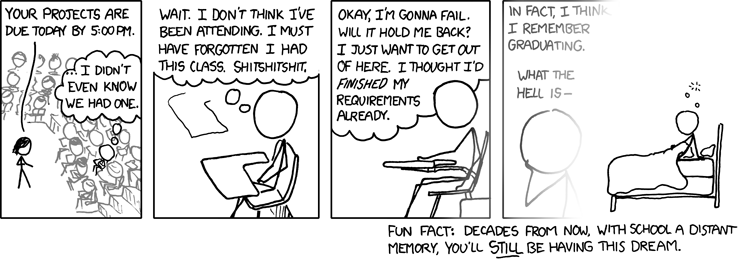
\includegraphics[scale=0.4]{comics/557}
\end{center}

\end{multicols}

\begin{multicols}{2}
\subsection*{Herzlich Willkommen!}

\textbf{Definition:} Ein Mensch am Anfang seines Mathematikstudiums heiße
Studienanfänger bzw.  Studienanfängerin.

\textbf{Bemerkung:} Der allgemeine Sprachgebrauch gestattet es, eine(n)
Studienanfänger(in) auch als Erstsemest(l)er(in) (kurz: Ersti) zu bezeichnen.

Es ist anschaulich klar, dass ein Studienanfänger bzw. eine Studienanfängerin,
da er (sie) per Definitionem noch nicht studiert, nicht wissen kann, worum es
eigentlich geht. Daraus motiviert sich folgender

\textbf{Satz und Definition:} Ein Studienanfänger bzw. eine Studienanfängerin
benötigt eine Orientierungshilfe. Diese Orientierungshilfe heiße
Orientierungseinheit (kurz: OE).

\textbf{Beweis:} Der elementare Beweis sei dem/der geneigten Leser(in) als
leichte Übungsaufgabe selbst überlassen.

\textbf{Bemerkung:} Da die Sinnfälligkeit des obigen Satzes selbst
hanseatischen Behörden geläufig ist, genügt man mit der Teilnahme an der OE dem
im Hamburgischen Hochschulgesetz, \S 52, Absatz 2 geforderten Besuch einer
Studienfachberatung in den ersten beiden Studiensemestern.

\subsection{Warum eine Orientierungseinheit?}

Jeder studienwütige Mensch hat früher voller Enthusiasmus am ersten Tag seines
Daseins als Student bzw. Studentin das Universitätsgebäude betreten und wusste
nicht: 

\begin{itemize}\itemsep 0pt
    \item Wo muss ich hin? Was soll ich tun? 
    \item Wie sieht mein Studium aus?
    \item Welche Vorlesungen sind zu besuchen?
    \item Wo kann ich mich dafür anmelden?
    \item Wie bekomme ich einen Schein?
    \item Wer sind meine Kommilitonen?
    \item Wo gibt es Essen?
    \item Wer kann mir bei Fragen und Problemen helfen?
\end{itemize}

Durch diese Orientierungslosigkeit ergab sich bei vielen Unmut oder
Frustration. Als Ergebnis haben manche das Studium vorzeitig abgebrochen oder
einige Semester an Zeit verloren, bevor sie alle Informationen beisammen
hatten, die für ihr Studium wichtig waren.

Um solch eine Situation zu verhindern, findet die Orientierungseinheit statt,
in der wir dir diese und noch viele andere Fragen beantworten oder zu
beantworten helfen.  Außerdem wollen wir 

\begin{itemize}\itemsep 0pt
    \item dir ein paar praktische Tipps zu deinem Studium geben,
    \item mit dir exemplarisch eine Studienwoche durchgehen,
    \item dir die Möglichkeit geben, deine Kommi\-litonen kennenzulernen, 
    \item dir zeigen, was sich alles hinter dem Begriff \glqq Mathematik\grqq\
          verbergen kann,
    \item dir alles mit einer Portion Humor und Witz servieren, sodass es allen
          Spaß macht.
\end{itemize}

Dabei solltest du wissen, dass die Orientierungseinheit von Studenten für
Studenten gemacht wird.  Alle guten Ratschläge und Tipps sind also kampferprobt
und gut gemeint.  Andererseits sind aber auch Angestellte der Hochschule dabei,
die darüber wachen, dass keiner Blödsinn erzählt. Des Weiteren ist jeder von
uns (Tutor oder Veranstalter) dabei, weil er eine solche Starthilfe für wichtig
hält.

Deine Teilnahme an der Orientierungseinheit ist freiwillig, das heißt du kannst
alternativ auch die gesamte Zeit zuhause bleiben.

\columnbreak

Dann fehlen dir aber wichtige
Informationen, die dir den Einstieg in das Studium erleichtern, du lernst keine
netten, neuen Leute kennen und verpasst eine Menge Spaß. Außerdem musst du im
Laufe deines Studiums sowieso an einer Studienfachberatung teilgenommen haben,
sonst erhältst du keinen Abschluss -- warum also nicht an dieser?!

\end{multicols}
\begin{center}
\vfill
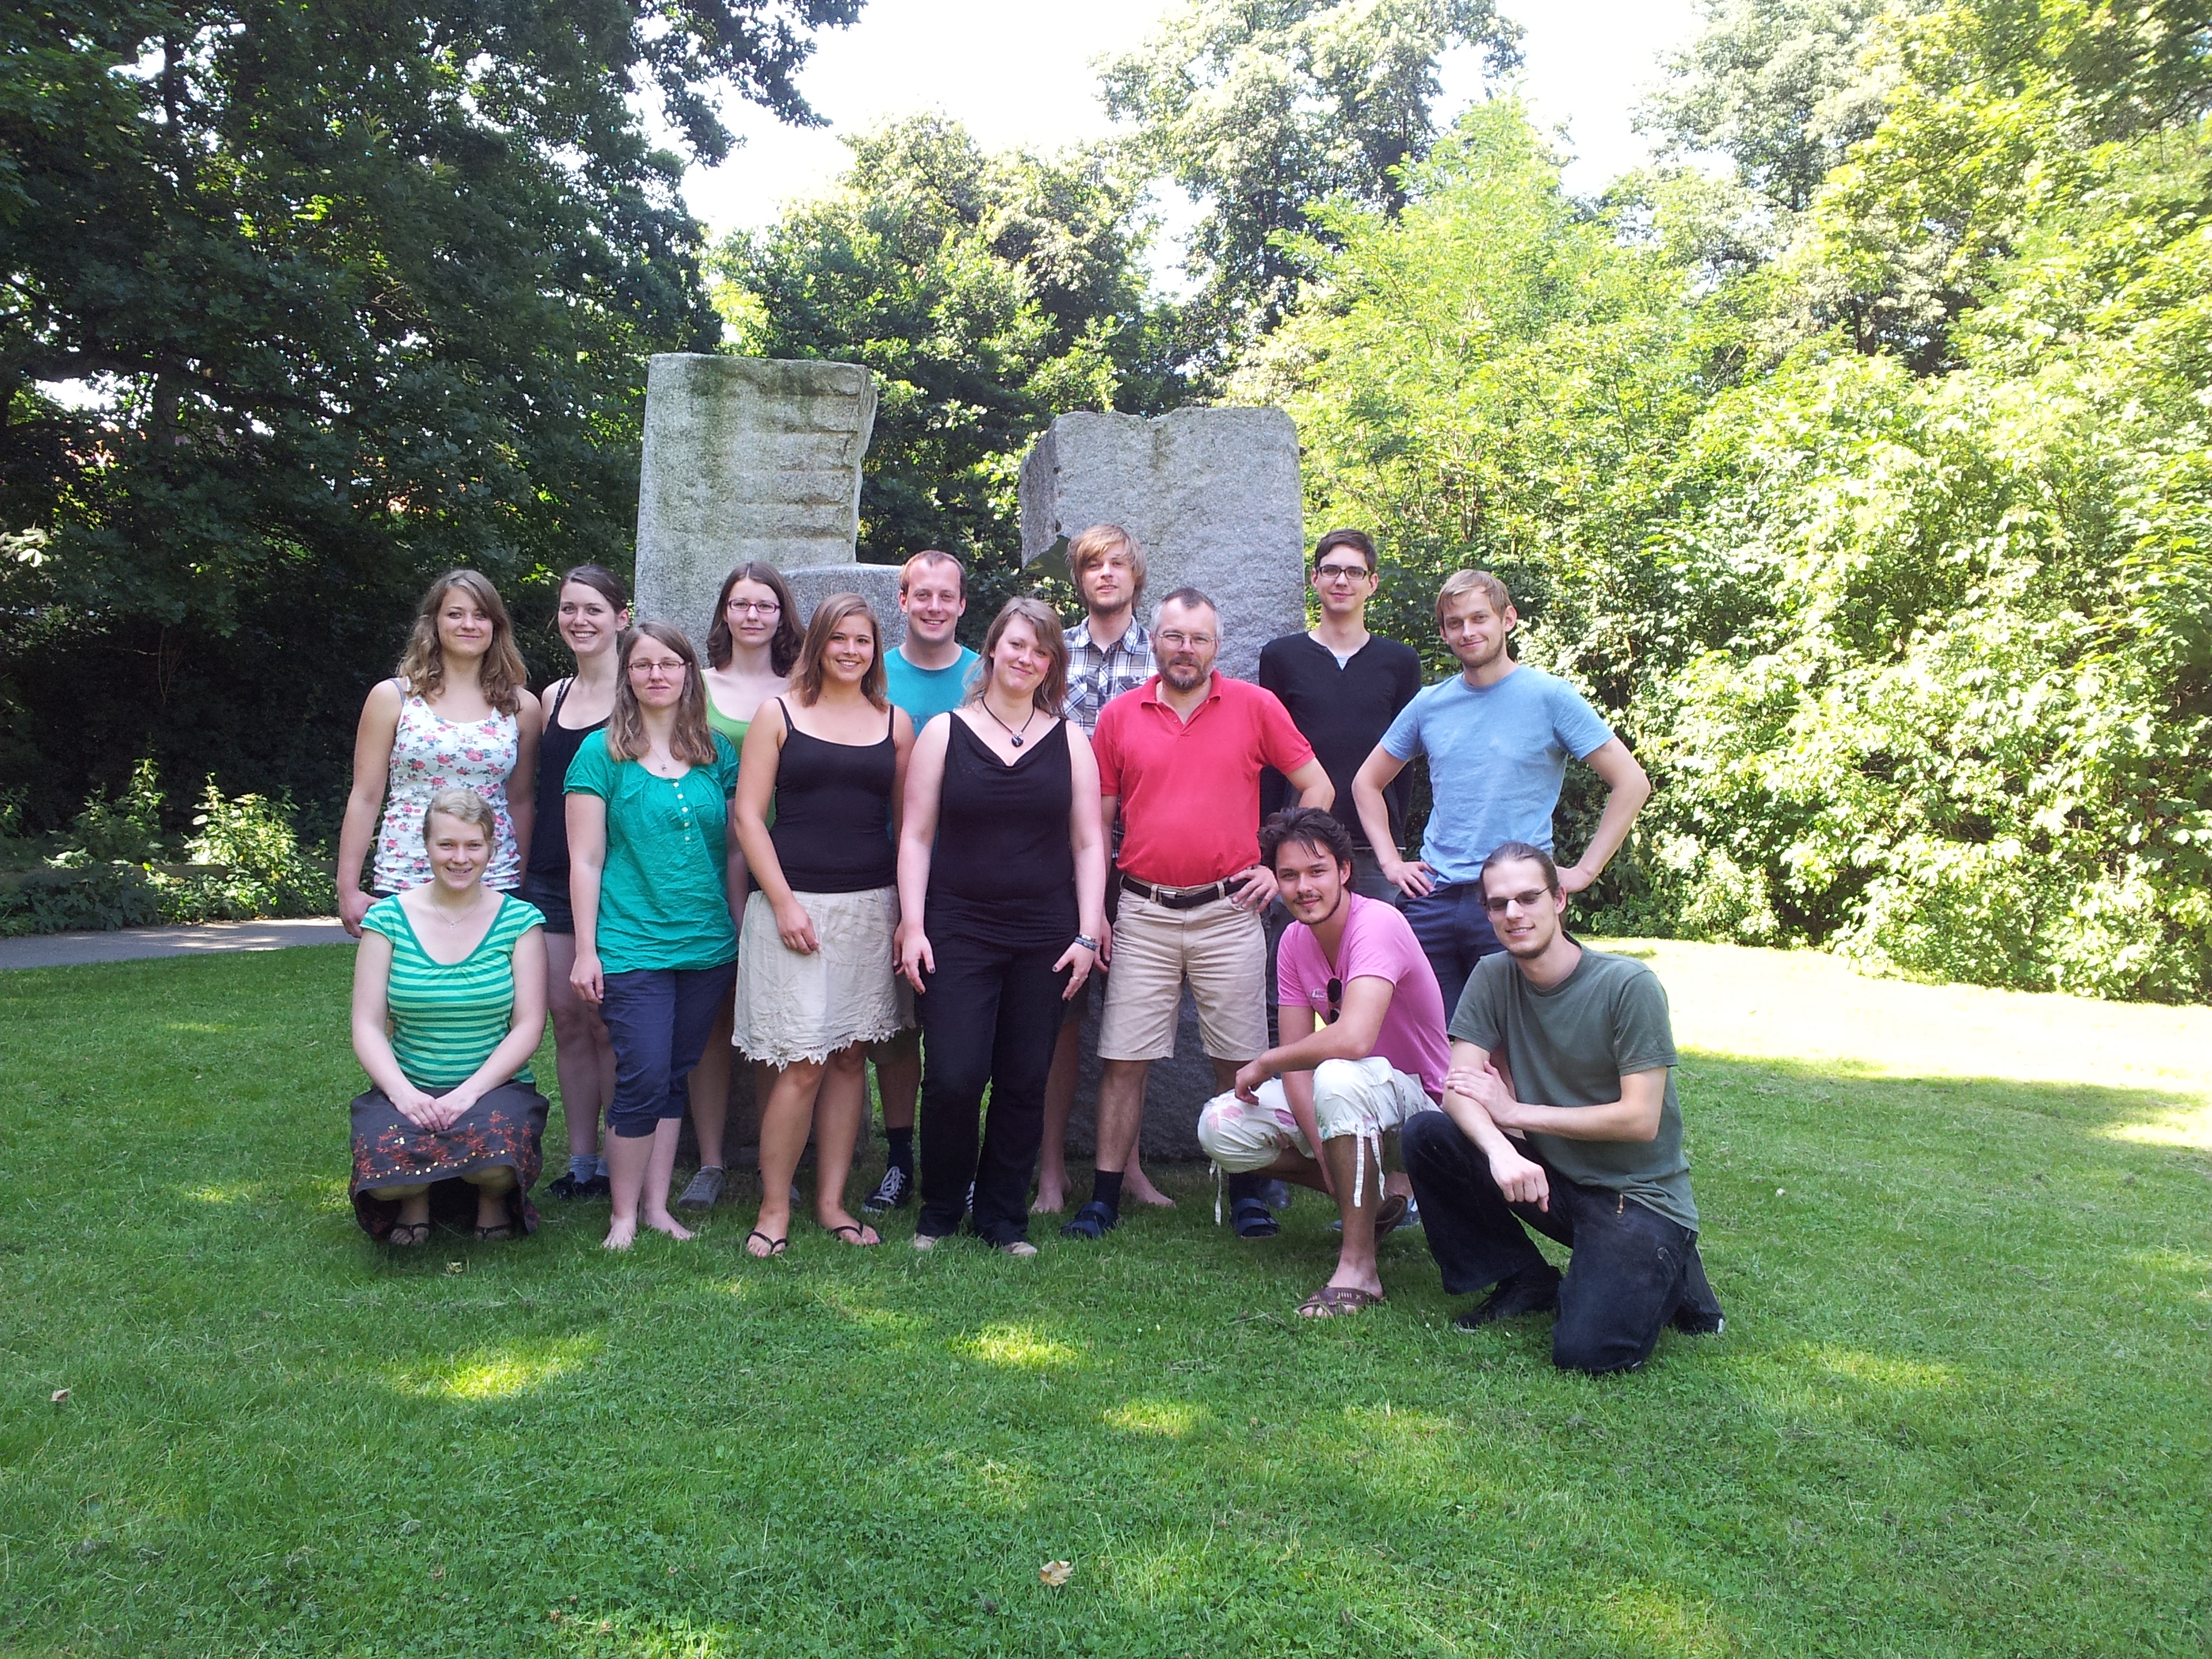
\includegraphics[width=195mm]{images/tutors.png}

\bigskip

\begin{minipage}{195mm}
Spaß bei der ganzen Orientierungseinheit wünschen dir

\hfill {\it die Tutorinnen, Tutoren und Veranstalter der Orientierungseinheit.}
\end{minipage}
\end{center}
\begin{multicols}{2}

\end{multicols}

\section{Was läuft in der OE?}
\begin{multicols}{2}
Bevor du erfährst, was in der OE passiert, erst einmal ein kurzer Hinweis, wie
die OE abläuft. Die OE findet nicht parallel zu deinen ersten
Mathematik-Vorlesungen statt, sondern davor. Sie ist fester Bestandteil der
Anfängerausbildung eines Mathematikers.  Auch Wirtschaftsmathematiker brauchen
keine Angst zu haben, dass sie etwas versäumen. Außerdem ist die
Orientierungseinheit so geplant, dass Studenten des Lehramts die ersten zwei
Tage an der Orientierungseinheit des Fachbereich Mathematik und anschließend an
der Orientierungseinheit der Erziehungswissenschaften teilnehmen können, ohne
etwas Wichtiges zu verpassen.

Die OE ist in Arbeitseinheiten gegliedert, was sich vielleicht etwas bedrohlich
anhört, aber ganz lieb gemeint ist und unter Umständen ganz lustig werden kann
(womit nicht gesagt sein soll, dass den Themen der ernste Hintergrund fehlt).
In jeder Arbeitseinheit soll, zumeist in Kleingruppen, ein bestimmter Aspekt
des (Mathematik-)Studiums behandelt und dir näher gebracht werden.

\subsection*{Studienberatung}

Wie dein Studium aufgebaut ist, welche Veranstaltungen du wann besuchst, wie du
am meisten aus den Veranstaltungen herausholst, wann gute Zeitpunkte für
Prüfungen sind und viele andere Informationen zum Studium und um das Studium
herum erhältst du in der Arbeitseinheit \emph{Studienberatung}. Alles, was
direkt mit den ersten Semestern zu tun hat, wird im ersten Teil am Montag,
den 08.10., behandelt.

Nur im Zusammenhang mit dem Rest der OE erfüllt die Teilnahme an dieser Einheit
die Anforderung des \S 51, Absatz 2 des Hamburgischen Hochschulgesetzes,
welcher besagt, dass jeder Student an einer Studienfachberatung teilgenommen
haben muss.

\subsection*{Lehr- und Lernformen}

An der Schule war alles so schön einfach: Der Lehrer kommt rein, erzählt ein
bisschen was -- und geht wieder raus. Meist sollte man dann zuhause zwei, drei
Aufgaben rechnen oder einige Seiten lesen. Das war's. Und verstanden habe ich
eh alles. Ich bin ja nicht blöd. Und in Mathe sogar gut!

An der Uni ist das ein bisschen anders: Es gibt Vorlesungen, Tutorien,
Übungsgruppen und noch einige Formen mehr. Was das ist? Nun, genau das wollen
wir dir zeigen, indem wir einen typischen Zyklus mit euch durchspielen: eine
Vorlesung, ein Tutorium, eine Übungsgruppe und zwei Arbeitsgruppen, in denen
wir mit dir die Vor- und Nachbereitung von Vorlesungen und das Lösen von
Aufgaben üben wollen.

Nein, wir halten dich nicht für völlig doof, aber an der Uni ist eben alles
etwas anders: Du wirst nicht mehr alles \glqq einfach so\grqq\ verstehen. Und
was dann? Wem stelle ich welche Fragen? Wozu brauche ich den
Übungsgruppenleiter? Was ist überhaupt der Unterschied zwischen Professor und
Dozent? Wie arbeite ich vor und nach, wie arbeite ich effizient in einer
Gruppe? Auf fast alle diese Fragen hat man eine Antwort parat. Und fast immer
ist sie falsch.

Diese Einheit soll euch den Umgang mit diesen Problemen zeigen, ohne dass ihr
den bitteren Weg des {\it trial and error} gehen müsst.

\subsection*{Q.E.D.}

Für einen erleichterten Einstieg in das erste Semester haben wir diese Einheit
ins Leben gerufen. Hier wollen wir mit dir die grundlegenden Dinge zum
korrekten Aufschreiben von Übungsaufgaben durchgehen, welche du dann auch
gleich für die Übungsaufgaben, die in der Einheit Lehr- und Lernformen gestellt
werden, nutzen kannst.

Diese Einheit umfasst einerseits einen Überblick über Beweismethoden, welche
wir auch gleich an einigen Beispielen üben wollen, andererseits einiges über
Logik und die Formulierung logischer Aussagen mithilfe von Junktoren, Quantoren
und Verknüpfungszeichen, welche dir in den ersten Semestern zahlreich begegnen
werden. Was sich hinter all diesen Begriffen versteckt, und dass dieses eher
hilfreiche als furchteinflößende Konzepte sind, wirst du hier lernen. (Und
auch, was \glqq q.e.d.\grqq\ bedeutet.)

Dabei soll die Einheit kein Versuch sein, den Besuch des ersten Semesters zu
ersetzen (das wäre in der kurzen Zeit auch gar nicht möglich). Wohl aber
möchten wir versuchen, dir den Einstieg zu erleichtern und insbesondere den
mühsamen Prozess, das korrekte Formulieren mathematischer Sachverhalte, ein
wenig zu vereinfachen.

\subsection*{Studentische Interessenvertretung}

Hinter dem sperrigen Begriff der \emph{Studentischen Interessenvertretung}
(SIV) verbirgt sich die einfache Idee, dass zum einen für alle Formen von
Problemen zuständige Anlaufstellen existieren, zum anderen die Universität von
der Mitbestimmung und gemeinsamen Gestaltung durch alle ihre Mitglieder lebt.
Hier gibt es für dich als Student vielfältige Möglichkeiten, dich zu engagieren
-- sowohl allgemein (hochschul-)politisch als auch auf fachlicher Ebene in den
einzelnen Fakultäten.

Alles dieses wollen wir am Mittwoch, den 10.10. in der Einheit SIV anhand
einiger Beispiele genauer betrachten. Weitere Informationen findest du auch im
IV-Artikel auf Seite \pageref{page:siv}.

\subsection*{Mathematik im Beruf}

Die wenigsten von euch, die Lehrämter ausgenommen, haben wohl schon konkrete
Vorstellungen davon, welchen Beruf sie ergreifen wollen und inwiefern sie das
Studium darauf vorbereitet. Um euch einen Einblick zu ermöglichen, welche
beruflichen Möglichkeiten es für Mathematiker und Wirtschaftsmathematiker gibt,
laden wir Berufstätige aus verschiedenen Branchen ein, die uns von ihrem
Berufsalltag erzählen und für Fragen zur Verfügung stehen.

Einen kleinen Einblick in die Nützlichkeit der Mathematik im heutigen Leben
gibt auch folgende Seite des Fachbereich:
\url{http://www.math.uni-hamburg.de/teaching2/Studieninteressierte/studieninteressierte.html}

\subsection*{Stadtführung}

Nicht nur für die Nicht-Hamburger ist dieser Programmpunkt gedacht.  Unter
Leitung unserer höchstkompetenten Tutoren wird unsere wunderschöne Stadt von
einer vielleicht ganz neuen Seite beleuchtet, und auch \glqq Eingeborene\grqq\
werden noch das eine oder andere neu entdecken; auf der \emph{Stadtführung} am
Donnerstag, 11.10. um 15:30 Uhr.

\subsection*{Mathematik und Gesellschaft}

Hält man sich längere Zeit unter Mathematikern auf, so kann man schnell zu dem
Eindruck gelangen, sie seien allesamt Wesen aus einer anderen Welt: Sie
sprechen eine eigene Sprache, lachen über eigene Witze und scheinen oftmals in
Gedanken in viel höheren Sphären zu schweben als in den Niederungen des
Alltags.  Und man kann sich die Frage stellen, ob Mathematiker und die
Mathematik überhaupt einen Bezug zu dieser Welt haben.


Um dich ein wenig auf dem Boden der Tatsachen zu halten, möchten wir diese
Frage zusammen mit dir in der Einheit \emph{Mathematik und Gesellschaft} (M\&G)
untersuchen. Auch im Artikel auf Seite \pageref{page:mug} finden sich weitere
Informationen und Gedanken zu diesem Thema. Denn gerade im Verlauf der ersten
Semester kann es manchmal ganz hilfreich sein, sich daran zu erinnern, dass man
auch nur ein menschliches Wesen und von dieser Welt ist.

\subsection{Erasmus}

% Anzahl der Partneruniversitäten und Länder.
% http://www.math.uni-hamburg.de/erasmus/partner.html.de

\emph{ERASMUS} ist ein europäisches Austauschprogramm, das Studierenden
ermöglicht, einmalig bis zu 10 Monaten an einer europäischen Partneruniversität
zu studieren. Insbesondere fördert ERASMUS die Mobilität von Studierenden und
Dozenten in Europa. Neben der Erweiterung der fachlichen Qualifikation soll der
Auslandsaufenthalt vor allem fremdsprachliche und interkulturelle Kompetenz
fördern. Studierende lernen dabei eine andere Perspektive kennen und sammeln
wertvolle persönliche Erfahrungen. Der Fachbereich Mathematik besitzt ERASMUS
Kooperationen mit mathematischen Fachbereichen aus 26 Partneruniversitäten in
12 europäischen Ländern.

Neugierig geworden? Weitere Informationen zum ERASMUS Programm, zu unseren
ERASMUS Partnern sowie zu den Teilnahmevoraussetzungen findet man auf der
Homepage \url{http://www.math.uni-hamburg.de/erasmus/}.

\subsection*{Abschlussfahrt nach Brahmsee}

Am Ende der Orientierungseinheit, vom 12. bis 13. Oktober, fahren wir mit euch
auf eine Abschlussfahrt nach Brahmsee. So kurz vor Studienbeginn wollen wir
noch zwei nette Tage mit euch verbringen. Am Freitag gibt es ein kleines
Tagesprogramm, sowie einen supercoolen \emph{Bunten Abend}, den wir schließlich
gemütlich am Lagerfeuer ausklingen lassen wollen. 

Während der ersten Tage geben alle Tutoren Listen herum, auf denen du bis
spätestens Montag, den 8.10., eintragen kannst, ob du mitkommst und
gegebenfalls ein Auto zur Verfügung hast, in dem noch Plätze frei sind. Die
Fahrt wird voraussichtlich etwa \EUR{30} pro Person kosten. Fahrer bekommen
jedoch eine großzügige Ermäßigung für jeden Mitfahrer. Damit deine Anmeldung
perfekt ist, möchten wir dich bitten, die Teilnahmegebühr bis spätestens Montag
bei einem der Tutoren zu zahlen.

Hier ist noch eine kleine Packhilfe. Das brauchst du unbedingt: 
\begin{itemize}\itemsep 0pt
    \item Bettlaken, Kopfkissenbezug und entweder einen Bettbezug oder
          Schlafsack
    \item Mindestens einen (gerne mehr!) Holzscheit(e) für ein großes
          Lagerfeuer, Taschenlampe
    \item deinen Lieblingsbrotbelag (Süßes gibt es!)
    \item was du sonst für eine Übernachtung brauchst 
\end{itemize}

Das kann mit: 
\begin{itemize}\itemsep 0pt
    \item Brett- und Kartenspiele
    \item Bälle, Frisbees, Tischtennisschläger, \dots
    \item Musikinstrumente
\end{itemize}

% TODO: Issue 4

Wir sehen uns Montag bei der Vorbesprechung! Dort kannst du alle deine Fragen
stellen und dich natürlich auch noch anmelden.

\end{multicols}
\begin{center}
\vfill

\includegraphics[scale=.8]{comics/435}
\end{center}
\begin{multicols}{2}

\end{multicols}

\section{Erste Fragen und Antworten}
\begin{multicols}{2}
\subsubsection{Der -- Die -- Das}

\dots\ Mathestudenten sitzen meist nur in der Vorlesung oder Übung und hören
zu.  Anscheinend verstehen sie alles, haben keine Fragen und keine Interessen,
die einer Vertretung nach außen wert wären.

\subsubsection{Wer -- Wie -- Was}

\dots\ ist denn da so an die Uni gekommen? Der Crack, der immer in der ersten
Reihe sitzt, ungehalten reagiert, wenn jemand den Prof mit Fragen aufhält und
scheinbar alles versteht.  Die Schöne, die sich täglich mindestens drei dumme
Sprüche anhören muss. Der Nerd, der immer seinen Laptop dabei hat. Die
Dozentin, die irgendwie zwei Meter über unserer Welt in Formeln schwebt. Die
beiden coolen Typen, die in der letzten Reihe über die gestrige Fete labern.
Der Kerl mit dem Rucksack, der immer eine Viertelstunde zu spät kommt. Die Type
mit dem Attach\'eeköfferchen (schweinsledern), die in der FAZ blättert.  Ich?

\subsubsection{Wieso -- Weshalb -- Warum}

\dots\ studieren wir eigentlich alle Mathe? \dots\ gibt es kaum eine
Professorin oder Dozentin am Fachbereich? \dots\ bin ich immer so schweigsam?
\dots\ frage ich so selten, obwohl mir doch so vieles unklar ist? \dots\ fällt
es mir so schwer, einfach meine Nachbarin zu fragen? \dots\ sitze ich jede
Woche alleine vor den Aufgaben? \dots\ geben 60 Prozent das Mathestudium auf,
bevor sie die ersten zwei Semester hinter sich haben? \dots\ kümmert sich hier
niemand um mich? \dots\ bin ich hier allen so egal?

\subsubsection{Wer nicht fragt bleibt dumm!}

So viele Fragen verlangen nach einer Antwort: 42! Aber hier wäre wohl doch eine
etwas konkretere Antwort angebracht. Leider kommt jetzt die große Enttäuschung:
In diesem Fall gibt es keine einzige oder richtige Antwort. Jeder entscheidet
einige Fragen für sich selbst, übernimmt andere aus dem Topf der allgemeinen
Meinung, tut sie als uninteressant ab oder macht sonst was mit seinem Wissen.
Warum denn nun die persönliche Meinung so oder so ausfällt, lässt sich ja auch
nicht immer begründen.

Die Universität ist ein derartiges Sammelsurium unterschiedlicher An- und
Einsichten -- was gerade am Fachbereich Mathematik trotz seiner geringen Größe
sehr ausgeprägt ist --, dass es der einzelnen Person nicht immer leicht fällt,
durch Wortgewandtheit und cooles Auftreten der anderen nicht irritiert oder
verunsichert zu werden. Das erfährt jeder mal am eigenen Leib, das ist kein
Bein- und schon gar kein Halsbruch. Ein Haken ist nur: Viele Neuankömmlinge
lassen sich schon in der OE dermaßen überrollen, dass sie kaum den Mund
aufbekommen. Die Vielfalt und Menge der neuen Eindrücke aus Uni und Umgebung
ist ja auch wahrlich unüberschaubar, gerade wenn eventuell auch noch der Umzug
in eine neue Stadt als Eindrucksquelle hinzukommt.

Da es auch immer wieder so ein paar unglaublich selbstsichere Hasskappen gibt,
die sich unter den merkwürdigsten Umständen weltgewandt und unbeeindruckt geben
können, bleibt meist die eigene Meinung ungehört. Unsinnigerweise sind es
nämlich gerade diese Personen, die als Orientierungshilfe dienen; meist ziehen
die auch nur eine gekonnte Show ab. Es soll ja Leute geben, die das
Fotografiertwerden vor dem Spiegel lernen.

Wichtig und studienbegleitend sollte folgender Merksatz sein: Keine Frage ist
zu dumm, um gestellt zu werden. Der feste Glaube, dass außer einem selbst
keiner diese Frage stellen würde, entpuppt sich fast immer als Irrglaube.
Sowieso sind die meisten Mitstudis für jede tempobremsende Frage überaus
dankbar. Es gibt kaum etwas Besseres für eine Vorlesung oder Übungsgruppe als
einer, der jede Behauptung hinterfragt. Bei einem Studium ist der Dialog
zwischen Lehrenden und Lernenden schließlich einer der Grundpfeiler für den
Erfolg.

Hinzu kommt, dass die Professoren sich über jede Bemerkung zu ihrer Tätigkeit
freuen werden. Erfahren sie doch auf diese Weise am ehesten etwas über ihre Art
zu unterrichten.

Und im Allgemeinen sind auch Professoren über so ein \glqq profanes\grqq\
menschliches Bedürfnis, wie es eine Reaktion nun einmal darstellt, nicht
erhaben!

\end{multicols}

\section{Informationen zu den Studiengängen}
\begin{multicols}{2}[\subsection{Der Bachelor-Studiengang}]

Seit dem Wintersemester 2006/07 sind die Studiengänge Mathematik und
Wirtschaftsmathematik an der Universität Hamburg, sowie die
Lehramtsstudiengänge auf das Bachelorsystem umgestellt.  Bevor wir euch auf den
nächsten Seiten die Studiengänge näher vorstellen wollen, werden wir euch vorab
ein paar grundlegende Informationen geben, die alle Studiengänge betreffen.
Alle Fragen, die sich vielleicht noch beim Lesen dieser Seiten ergeben, könnt
ihr am besten während der Studienberatung stellen, aber auch darüber hinaus
sind die Tutoren für alle Fragen rund um das neue Bachelorstudium ansprechbar.
Im Internet findet ihr die aktuellsten Informationen unter
\url{http://www.math.uni-hamburg.de/teaching2/index.html}

\subsubsection{Der grobe Überblick}

Das Studium ist auf 6 Semester ausgelegt. Anschließend kann man sich für einen
der weiterführenden Master-Studiengänge, ausgelegt auf vier Semester,
entscheiden oder auch direkt in das Berufsleben starten. Für Lehramtsstudenten
ist dabei ein Master nötig um an Schulen unterrichten zu dürfen.

Das Bachelorstudium ist in \emph{Module} organisiert. Ein Modul kann mehrere
Veranstaltungen, \emph{Vorlesungen}, \emph{Seminare}, \emph{Übungen}, umfassen,
die inhaltlich zusammenhängen.  Jedes Modul wird mit einer \emph{Prüfung}
abgeschlossen.  Die Ergebnisse der meisten Modulprüfungen gehen in die
Abschlussnote ein. In manchen Fällen werden Teilmodulprüfungen abgenommen.
Details über die einzelnen Module findet ihr in den \emph{Fachspezifischen
Bestimmungen} (FSB) der jeweiligen Fächer.  Es gibt \emph{Pflichtmodule},
\emph{Wahlpflichtmodule}, \emph{Ergänzungsmodule} und frei wählbare
\emph{Wahlmodule}.  Dabei kann ein Modul auch über zwei Semester gehen wie zum
Beispiel die Analysis- oder die Lineare Algebra \& Analytische
Geometrie-Vorlesung. 

In den ersten Semestern habt ihr bei der Belegung im mathematischen Bereich
nicht sehr viele Möglichkeiten das Studium nach euren Vorstellungen zu
gestalten.  Das wird in der zweiten Studienphase mit der Wahl der
Wahlpflichtmodule einfacher.  Im Vergleich mit anderen mathematischen
Fachbereichen zeichnet sich dabei der Fachbereich Mathematik an der Universität
Hamburg durch eine besonders große Vielfalt aus, die sich in der fachlichen
Breite der Schwerpunkte widerspiegelt. Somit habt ihr bei der Wahl eurer
Wahlpflichtmodule vielzählige Angebote

Eure Module im Bereich Mathematik sind meist mit einer Vorlesung und einer
zugehörigen Übung aufgebaut.  In den Übungsstunden werden die Übungsaufgaben zu
den Vorlesungen verteilt und besprochen.  Die Übungen sind wichtig, da ihr euch
zum Lösen der Aufgaben mit dem späteren Prüfungsstoff beschäftigen müsst, aber
auch, weil das erfolgreiche Lösen der Übungsaufgaben in der Regel eine
Zulassungsvoraussetzung für die Modulabschlussprüfung ist.  Des Weiteren ist
ein wichtiger Bestandteil der Übungen das Vortragen der Hausaufgaben vor der
Gruppe an der Tafel.  Auch dieses kann eine Zulassungsvoraussetzung sein. Die
genauen Bestimmungen wird der jeweilige Veranstalter zu Beginn des Semesters
bekannt geben.  Zusätzlich wird in der Analysis und der Linearen Algebra \&
Analytischen Geometrie noch ein freiwilliges \emph{Tutorium} angeboten, in
welchem die Inhalte der Vorlesung wiederholt und vertieft und Fragen
beantwortet werden.

% TODO: Erklärung von SWS analog zu LP.
Alle Module sind mit einer bestimmten Anzahl an \emph{Leistungspunkten} (LP)
bewertet. Diese geben einen Eindruck vom Arbeitsaufwand, der zum erfolgreichen
Absolvieren des Moduls notwendig ist. Ein Richtwert hierfür sind etwa 30
Arbeitsstunden pro Leistungspunkt.  Vorgesehen sind etwa 30 LP pro Semester und
180 LP bis zur Beendigung des Bachelorstudiums.  Es ist normal, dass man in dem
einen Semester ein paar LP mehr und im anderen Semester ein paar LP weniger
macht, es ist aber eine Gleichverteilung der Punkte sinnvoll.  Der Zeitumfang
einer Veranstaltung wird in \emph{Semesterwochenstunden} (SWS) ausgedrückt.

Im weiteren Verlauf eures Studiums werdet ihr auch Seminare belegen.  In
Seminaren erarbeitet man vorgegebene Themen anhand von Literatur und hält vor
den Seminarteilnehmern einen Vortrag über sein Thema.  Um dieses zu üben, gibt
es \emph{Proseminare}, die euch einen guten Einstieg in diese Arbeitsweise
geben sollen. Im Studium Bachelor Mathematik und Bachelor Wirtschaftsmathematik
ist ein Proseminar verpflichtend vorgesehen. 
\end{multicols}

\clearpage

\begin{multicols}{2}[\section{Bachelor Mathematik}]

In den ersten drei Semestern, die zur \emph{ersten Studienphase} gehören,
werden euch in Pflichtmodulen die mathematischen Grundlagen in den Bereichen
Analysis, Lineare Algebra, Numerische Mathematik und Mathematische Stochastik
vermittelt. Zusätzlich müsst ihr die Module zum Erlernen allgemeiner
berufsqualifizierende Kompetenzen (ABK) \emphm{Programmiermethoden} und
\emphm{Softwarepraktikum} belegen. Abgeschlossen wird die erste Studienphase
durch ein Proseminar, das für das vierte Semester vorgesehen ist.  In der
\emph{zweiten Studienphase}, viertes bis sechstes Semester, könnt ihr den
mathematischen Teil eures Studiums aus einer Vielzahl von Wahlpflichtmodulen
nach euren persönlichen Neigungen selber gestalten. 

In diesem Wintersemester hört ihr neben zwei Veranstaltungen aus der reinen
Mathematik, \emphm{Analysis I} und \emphm{Lineare Algebra \& Analytische
Geometrie I}, Vorlesungen in eurem \emph{Ergänzungsfach}. Im 2. Semester hört
ihr \emphm{Analysis II}, \emphm{Lineare Algebra \& Analytische Geometrie II}
sowie eventuell eine weitere Veranstaltung eures Ergänzungsfaches oder besucht
eine kleinere Veranstaltung aus der Mathematik. In den letzten Wochen vor
Beginn des dritten Semesters müsst ihr noch einen Programmierkurs absolvieren,
der euch auf die Veranstaltung \emphm{Numerische Mathematik} vorbereitet. Das
3.  Semester setzt sich dann aus den Veranstaltungen \emphm{Höhere Analysis},
\emphm{Mathematische Stochastik} und \emphm{Numerische Mathematik} sowie einem
\emphm{Softwarepraktikum} zusammen. 

Der Umfang der einzelnen Veranstaltungen sieht wie folgt aus: Alle oben
genannten Mathematik-Module bestehen aus 4 SWS Vorlesung und 2 SWS Übung.
Begleitend zu den Modulen \emphm{Analysis} und \emphm{Lineare Algebra \&
Analytische Geometrie} wird ein freiwilliges 2 SWS Tutorium angeboten. Der
Programmierkurs findet als zweiwöchiger Blockkurs am Ende der vorlesungsfreien
Zeit statt. Die Inhalte des Softwarepraktikums sollt ihr euch selbstständig
erarbeiten, zeitlich neben den Mathematik-Vorlesungen. Im Softwarepraktikum
gibt es keine Vorlesung oder Übung, sondern nur eine Sprechstunde bei
Problemen.

In der zweiten Studienphase habt ihr die Möglichkeit, euch euren Interessen
entsprechend auszurichten. Dabei müsst ihr aus einem großen Kanon an
Wahlpflichtveranstaltungen des Bachelors Module im Umfang von insgesamt 36 LP
sowie im vieten Semester ein Proseminar und im fünften Semester ein Seminar
belegen. Bei der Auswahl der Module sollte auf einen \emph{sinnvollen
Studienaufbau} und eine \emph{hinreichende Breite} geachtet werden.  Im dritten
Semester findet eine verpflichtende \emph{Studienfachberatung} statt, die euch
darüber informieren soll, was genau sich hinter diesen Begriffen verbirgt.
Während eures Studiums solltet ihr ein Berufspraktikum absolvieren. Alternativ
könnt ihr dieses ABK-Modul jedoch auch durch das Leiten einer Übungsgruppe oder
durch die Arbeit an einem Projekt abdecken.  Die zweite Studienphase wird durch
die Bachelorarbeit abgeschlossen. Diese baut in der Regel auf einem
Wahlpflichtmodul oder dem Seminar auf.

% Referenz
Zusätzlich zu den Mathematik-Vorlesungen müsst ihr noch Veranstaltungen in
einem Ergänzungsfach belegen, in dem ihr die Grundlagen eines wichtigen
Anwendungsgebiets der Mathematik kennen lernt. Dieses ist ein Fach mit einem
direkten Bezug zur Mathematik, das ab dem 1. Semester gehört werden sollte. Auf
Seite 13 des OE-Laptops wirst du umfassend über die Ergänzungsfächer
informiert.

Das Modulspektrum des Bachelor wird durch den \emph{Wahlbereich}
vervollständigt. Prinzipiell stehen euch dafür alle an der Universität Hamburg
angebotenen Veranstaltungen zur Verfügung.  In eurem eigenen Interesse solltet
ihr jedoch auf eine sinnvolle Verteilung der 21 LP Wert legen. So ist es nicht
nur wenn ihr ein Masterstudium an den Bachelor anschließen wollt vernünftig,
einen Teil der Wahlmodule mit Mathematikveranstaltungen oder zusätzlichen
Veranstaltungen im Ergänzungsfach abzudecken.  Doch auch das Belegen von
Sprach- oder Computerkursen kann zur zusätzlichen Qualifikation für euren
späteren Traumjob sinnvoll sein.
\end{multicols}
\clearpage

\subsection{Musterstudienplan für den Studiengang B.Sc. Mathematik}

\begin{center}
\begin{tabular}{||l||l|l|l|l|l|l||}
\hhline{|t:=:t:=t=t=t=t=t=:t|}
\hspace*{25mm} & 1. Semester\hspace*{8ex} & 2. Semester\hspace*{8ex} & 3. Semester\hspace*{8ex} & 
4. Semester\hspace*{8ex} & 5. Semester\hspace*{8ex} & 6. Semester\hspace*{8ex} \\
\hhline{|:=::======:|}
Pflichtbereich & Analysis I& Analysis II&Höhere Analysis& Proseminar &Seminar& Bachelorarbeit\\
\hhline{||~||~|~|~|~|~|~||} &(9 LP)&(9 LP)&(9 LP)&(4 LP) &(6 LP)& (12 LP)\\
\hhline{||~||~|~|~|~|~|~||} &&&&&&\\
\hhline{||~||~|~|~|~|~|~||} &Lineare Algebra & Lineare Algebra & Mathematische & & &\\ 
\hhline{||~||~|~|~|~|~|~||} &und Analytische & und Analytische & Stochastik & & &\\ 
\hhline{||~||~|~|~|~|~|~||} &Geometrie I&Geometrie II & (9 LP) & &&\\ 
\hhline{||~||~|~|~|~|~|~||} &(9 LP)&(9 LP)& &&&\\
\hhline{||~||~|~|~|~|~|~||} &&&Numerische&&&\\
\hhline{||~||~|~|~|~|~|~||} &&&Mathematik&&&\\
\hhline{||~||~|~|~|~|~|~||} &&&(9 LP)&&&\\ 
\hhline{||~||~|~|~|~|~|~||} &&&&&&\\
\hhline{|:=::======:|}
\hhline{||~||~|~|~|~|~|~||} Wahlpflicht-&&&&Vertiefungs-&Vertiefungs-&Vertiefungs- \\
\hhline{||~||~|~|~|~|~|~||} bereich&&&&module&module&module \\
\hhline{||~||~|~|~|~|~|~||} &&&&(18 LP)&(9 LP)&(9 LP) \\
\hhline{||~||~|~|~|~|~|~||} &&&&&&\\
\hhline{|:=::======:|}
ABK-Bereich&& Programmier-&Softwarepraktikum&&Betriebspraktikum/& \\
\hhline{||~||~|~|~|~|~|~||} &&methoden&(4 LP)&&Projekt/Tutorium&\\
\hhline{||~||~|~|~|~|~|~||} &&(5 LP)&&&(5 LP)&\\
\hhline{||~||~|~|~|~|~|~||} &&&&&&\\
\hhline{|:=::======:|}
Ergänzungs-&Ergänzungs- &Ergänzungs-&&&Ergänzungs-&Ergänzungs-\\
\hhline{||~||~|~|~|~|~|~||} fachbereich&fachmodule&fachmodule&&&fachmodule&fachmodule\\
\hhline{||~||~|~|~|~|~|~||} &(7 LP)&(3 LP)&&&(5 LP)&(9 LP)\\
\hhline{||~||~|~|~|~|~|~||} &&&&&& \\
\hhline{|:=::======:|}
Wahlbereich&Wahlmodul&Wahlmodul&&Wahlmodul&Wahlmodul&\\
\hhline{||~||~|~|~|~|~|~||} &(4 LP)&(4 LP)&&(8 LP)&(5 LP)&\\
\hhline{||~||~|~|~|~|~|~||} &&&&&& \\
\hhline{|b:=:b:======:b|}
\end{tabular}
\end{center}

\clearpage

\begin{multicols}{2}
% TODO: Diese Datei sollte in die Einleitung und die einzelnen Ergänzungsfächer
% gesplittet werden.

\subsection{Ergänzungsfächer} \label{page:erg}

Die Studienordnung für den Studiengang Bachelor Mathematik sieht vor, dass sich
die Studierenden nicht nur auf die Mathematik konzentrieren, sondern auch ein
Ergänzungsfach belegen, welches einen starken Bezug zur Mathematik aufweist.
Die klassischen Ergänzungsfächer sind Physik, Informatik, Technik, Betriebs-
und Volkswirtschaftslehre. In den letzten Jahren kamen noch Chemie, Philosophie
und Geographie zu den gängigen Ergänzugsfächern hinzu. Falls ihr bereits zu
Beginn des Studiums plant, in Hamburg ein Masterstudium in einem der hier
geplanten interdisziplinären Studiengänge (Technomathematik, Mathematische
Physik oder Wirtschaftsmathematik) anzuschließen, wird empfohlen, das
Ergänzungsfach entsprechend zu wählen, denn es ist sehr wahrscheinlich, dass
die Masterstudiengänge hier spezielle Kenntnisse voraussetzen werden.

Zu den oben genannten Ergänzungsfächern existieren schon Studienpläne, die
Aussagen darüber machen, welche Vorlesungen belegt werden müssen. Falls ihr
aber unbedingt ein anderes Ergänzungsfach wählen wollt (zum Beispiel
Astronomie, Psychologie, Soziologie, Musikwissenschaften oder Gender Studies),
das nicht zu den im Internet aufgeführten gehört, so müsst ihr euch selber
darum kümmern und dies mit dem Studienbüro Mathematik (Seite
\pageref{studienburo}) absprechen. Im folgenden haben wir für euch die
klassischen Ergänzungsfächer noch einmal aufgeführt und zu jedem ein paar
weitere Erklärungen geliefert, die euch bei der Wahl helfen sollen.

Genauere Informationen zu den fünf klassischen Ergänzungsfächern erhaltet ihr
am Dienstag, 9.10. um 11:00 Uhr in der Einheit Ergänzungsfächer. Dort habt ihr
dann die Möglichkeit, erfahrene Tutoren mit Fragen zu den Fächern zu löchern
oder ihnen zuzuhören, wie sie aus dem Nähkästchen plaudern.

\subsubsection{Informatik}

Wenn ihr mit dem Computer umgehen könnt und in der Schule vielleicht auch schon
einmal programmiert habt, dann ist Informatik eine interessante Möglichkeit für
euer Ergänzungsfach. Auch profitiert ihr spätestens im 2. und 3.  Semester bei
der Numerischen Mathematik von eurer Wahl, denn ein Teil der Aufgaben, die ihr
für Numerik lösen müsst, sind Programmieraufgaben. Beim Ergänzungsfach
Informatik sind regelhaft Module im Gesamtumfang von (wenigstens) 24 LP aus den
folgenden vom Fachbereich Informatik angebotenen Modulen zu absolvieren. In
Klammern sind die Kennungen der Module angegeben.

\begin{itemize}\itemsep 0pt
    \item Softwareentwicklung I (IP1, 6 LP)
    \item Softwareentwicklung II (IP2, 9 LP)
    \item Softwareentwicklung III (IP3, 6 LP)
    \item Algorithmen und Datenstrukturen (IP4, 6 LP)
    \item Grundlagen von Datenbanken (IP5, 6 LP)
    \item Grundlagen der Systemsoftware (IP6, 6 LP)
    \item Rechnerstrukturen (IP7, 9 LP)
    \item Formale Grundlagen der Informatik I (IP8, 9 LP)
    \item Formale Grundlagen der Informatik II (IP9, 9 LP)
\end{itemize}

Besonders empfohlen wird die Modulkombination \emphm{Softwareentwicklung~I},
\emphm{Softwareentwicklung~II} und \emphm{Formale Grundlagen der Informatik~I}.
\begin{wrapfigure}{r}{52mm}
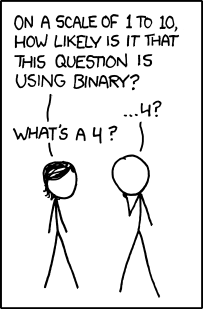
\includegraphics[scale=.8]{comics/953}
\end{wrapfigure}

Für das Modul \emphm{Formale Grundlagen der Informatik I} kann es hilfreich
sein vorher oder parallel das mathematische Wahlpflichtmodul \emphm{Diskrete
Mathematik} gehört zu haben.

Während die Vorlesungen noch auf dem großen Uni-Campus, meist im
Philosophenturm, stattfinden, müsst ihr euch spätestens zu den Übungen in das
Informatikum nach Stellingen begeben. Die Fahrt dauert vom Schlump aus etwa 15
Minuten (U2 bis Hagenbecks Tierpark und dann Bus 181 oder 281 bis zum
Informatikum). Falls ihr noch weitere Fragen zu Informatik als Ergänzungsfach
habt, können euch der FSR Informatik
(\url{www.informatik.uni-hamburg.de/Fachschaft/}) oder eure Tutoren
weiterhelfen.

\clearpage

\subsubsection{Physik}

Beim Ergänzungsfach Physik ist regelhaft alternativ eine der
beiden folgenden Modulkombinationen zu absolvieren:

\begin{itemize}\itemsep 0pt
    \item Physik 01 (12 LP)
          \begin{itemize}\itemsep 0pt
              \item Physik I (6 LP)
              \item Einführung in die Theoretische Physik I (6 LP)
          \end{itemize}
    \item Theoretische Physik I (Klassische Feldtheorie) (9 LP)
    \item ein physikalisches Proseminar (3 LP)
\end{itemize}
oder
\begin{itemize}\itemsep 0pt
    \item Experimentalphysik I (für Studierende d. Chemie, Lebensmittelchemie,
    Mathematik 6 LP)
    \item Theoretische Physik I (Klassische Feldtheorie) (9 LP)
    \item Theoretische Physik II (Quantenmechanik) (9 LP)
\end{itemize}

Ihr solltet schnell Lerngruppen mit Physikern bilden.  Erfahrungsgemäß könnt
ihr besser beweisen und die besser rechnen. Physik ist nicht gerade das
einfachste Ergänzungsfach, wohl aber dasjenige, bei dem ihr sicher seid, etwas
gemacht und gelernt zu haben. Bei Fragen könnt ihr euch auch an den FSR Physik
(\url{www.physnet.uni-hamburg.de/fs/}) wenden.

\subsubsection{Chemie}

Falls du gerne Chemie im Nebenfach zu deinem Mathematik-Studium wählen
möchtest, sind regelhaft die folgenden Module zu absolvieren.

\begin{itemize}\itemsep 0pt
    \item Grundlagen der Allgemeinen Chemie (CHE 80)
    \item Organische Chemie für Studierende mit Chemie im Nebenfach  (CHE 81)
    \item Physikalische Chemie und Mathematik (CHE 02)
\end{itemize}

Die Module \emphm{Grundlagen der Allgemeinen Chemie} und \emphm{Physikalische
Chemie und Mathematik} werden regelmäßig im Wintersemester und das Modul
\emphm{Organische Chemie für Studierende mit Chemie im Nebenfach} im
Sommersemester angeboten. Weitere Informationen zu den Modulen kannst du auf
der folgenden Seite des Fachbereichs Chemie finden.
\url{http://www.chemie.uni-hamburg.de/studiengaenge.html}

\subsubsection{Geographie}

In dem Nebenfach Geographie werden regelhaft die folgenden Module angeboten.

\begin{itemize}\itemsep 0pt
    \item Anthropogeographie A
    \item Anthropogeographie B
    \item Physische Geographie A
    \item Physische Geographie B
    \item Geodatenanalyse: Einführung
    \item Fachmethodik I (Lehramt)
\end{itemize}

Ihr könnt euch aussuchen, ob ihr \emphm{Anthropogeographie A} und \emphm{B}
oder \emphm{Physische Geographie A} und \emphm{B} belegt und ob ihr euer
Ergänzungsfach mit \emphm{Geodatenanalyse: Einführung} oder \emphm{Fachmethodik
I} vervollständigt.  Weitere Informationen findest du unter
\url{http://www.uni-hamburg.de/geowissenschaften/}.

\begin{center}
\vfill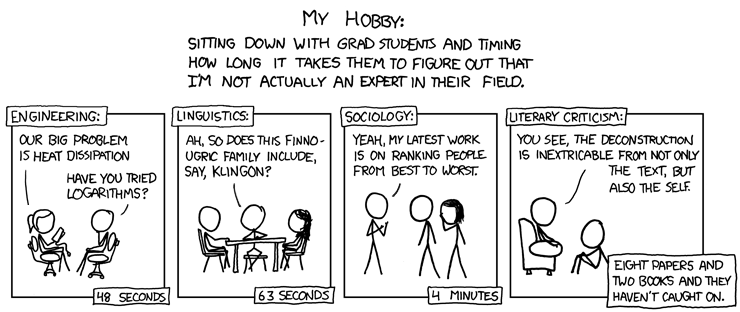
\includegraphics[scale=.5]{comics/451}
\end{center}

\subsubsection{Betriebswirtschaftslehre}

Die Betriebswirtschaftlehre (BWL) ist eine Disziplin der
Wirtschaftswissenschaften, die sich mit den wirtschaftlichen Entscheidungen in
Betrieben und Unternehmen befasst, vor allem mit Art und Menge der zu
beschaffenden Produktionsmittel, Beschaffung und Verwendung der Finanzmittel,
Einsatz der beschafften Produktionsmittel und Veräußerung der Erzeugnisse und
Leistungen. Beim Ergänzungsfach BWL sind regelhaft die folgenden Module zu
absolvieren, die vom Fachbereich Wirtschaftswissenschaften angeboten werden:

\begin{itemize}\itemsep 0pt
    \item Grundlagen des Rechnungswesens (6 LP)
    \item Kosten- und Leistungsrechnung (3 LP)
    \item Unternehmensführung I (3 LP)
    \item Grundzüge der Finanzwirtschaft
          \begin{itemize}\itemsep 0pt
              \item Investition (6 LP)
              \item Finanziernug (6 LP)
          \end{itemize}
\end{itemize}

Bei Fragen wendet euch an eure Tutoren oder an den FSR
Wirtschaftswissenschaften (\url{http://www.wiwifsr.de}).

\begin{center}
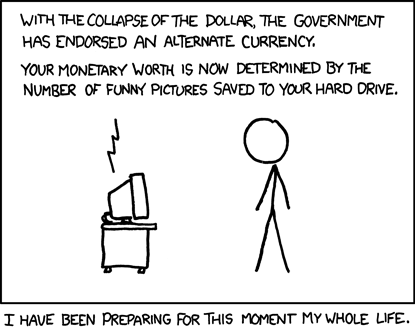
\includegraphics[scale=.675]{comics/512}
\end{center}

\subsubsection{Volkswirtschaftslehre}

Die Volkswirtschaftslehre (VWL) teilt sich in die Wirtschaftstheorie (Mikro-
und Makroökonomie), die Wirtschaftspolitik, die Finanzwissenschaft und die
Wirtschafts- und Dogmengeschichte auf. Dabei versucht die VWL, abgelaufene
wirtschaftliche Vorgänge auf einzel- und gesamtwirtschaftlicher Ebene zu
beschreiben, eine beobachtete wirtschaftliche Lage mittels ökonomischer
Theorien zu erklären, Prognosen über zukünftige wirtschaftliche Vorgänge zu
machen und eine wirtschaftspolitische Beraterfunktion einzunehmen.  Beim
Ergänzungsfach VWL sind regelhaft die folgenden Module zu absolvieren, die vom
Fachbereich Wirtschaftswissenschaften angeboten werden:

\begin{itemize}\itemsep 0pt
    \item Mikro- und Makroökonomische Theorie
        \begin{itemize}\itemsep 0pt
              \item Mikroökonomik (6 LP)
              \item Makroökonomik (6 LP)
        \end{itemize}
    \item Ökonometrie
          \begin{itemize}\itemsep 0pt
              \item Angewandte Ökonometrie I (6 LP)
              \item Angewandte Ökonometrie II (6 LP)
          \end{itemize}
\end{itemize}

Auch hier könnt ihr euch natürlich bei Fragen an die Tutoren oder den FSR
Wirtschaftswissenschaften wenden.

\subsubsection{Philosophie}

Ein nach landläufiger Meinung klassisches Nebenfach für die Mathematik ist die
Philosophie. An der Universität Hamburg wird dieses Nebenfach seit neuem
regelhaft angeboten. Ihr habt dabei die Wahl zwischen einem eher theoretischen
oder einem eher praktischen Zugang zu diesem Nebenfach. Die vorgeschlagenen
Modulkombinationen der theoretischen Variante sind

\begin{itemize}\itemsep 0pt
    \item Einführungsmodul Logik und Argumentationstheorie 
    \item Einführungsmodul Praktische Philosophie: Ethik 
    \item Einführungsmodul Theoretische Philosophie 
    \item Aufbaumodul Theoretische Philosophie 
\end{itemize}

\columnbreak

Für die praktische Variante werden die folgende Module vorgeschlagen.

\begin{itemize}\itemsep 0pt
    \item Einführungsmodul Logik und Argumentationstheorie 
    \item Einführungsmodul Praktische Philosophie: Ethik 
    \item Einführungsmodul Theoretische Philosophie 
    \item Aufbaumodul Praktische Philosophie
\end{itemize}

\subsubsection{Technik}

Die Vorlesungen im Ergänzungsfach Technik werden von der Technischen
Universität Hamburg Harburg (TUHH) angeboten. Die TU liegt in der Nähe der
S-Bahn Harburg-Rathaus, und ihr müsst eine gute halbe Stunde Zeit einplanen, um
vom Geomatikum aus dorthin zu gelangen. Regelhaft sind die folgenden Module zu
absolvieren:

\begin{itemize}\itemsep 0pt
    \item Technische Mechanik 1 (4,5 LP)
    \item Technische Mechanik 2 (4,5 LP)
    \item Grundlagen der Elektrotechnik 1 (7,5 LP)
    \item Grundlagen der Elektrotechnik 2 (7,5 LP)
\end{itemize}

Behandelte Themen der Vorlesungen \emphm{Technische Mechanik 1} und \emphm{2}
sind Starrkörperstatik, Elastostatik, Fluidstatik, Kinematik und Kinetik.
\emphm{Grundlagen der Elektrotechnik 1} behandelt Gleichstrom, während der
zweite Teil sich der Wechselstromlehre widmet. Die theoretische Grundlage
dieser beiden technischen Bereiche sowie die Beschreibung ihrer
Gesetzmäßigkeiten sind eng mit verschiedenen Disziplinen der Mathematik
verknüpft. Bei Fragen könnt ihr euch an den FSR Maschinenbau
(\url{www.tu-harburg.de/exp/fsrm}) für Mechanik, den FSR Elektrotechnik
(\url{www.fsr-etit.de}) oder an die Tutoren wenden.

\begin{center}
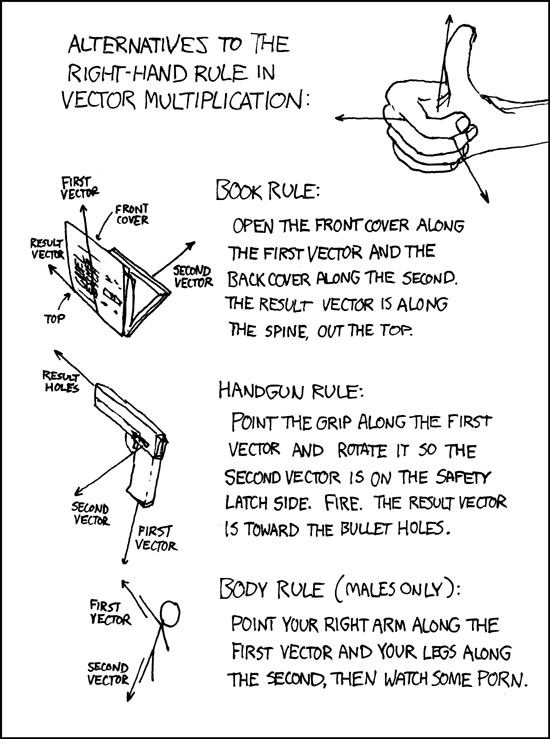
\includegraphics[scale=.66]{comics/199}
\end{center}

\end{multicols}
\begin{multicols}{2}[\section{Bachelor Wirtschaftsmathematik}]

Der Bachelor Wirtschaftsmathematik ist durch die Fachspezifischen Bestimmungen
(FSB) in einen mathematischen, einen wirtschaftlichen und einen praxisbezogenen
Bereich gegliedert, in denen ihr bestimmte Leistungen erbringen müsst. In einem
vierten Bereich könnt ihr euer Studium nach euren Vorstellungen ausbauen, indem
ihr einen oder mehrere obligatorische Bereiche vertieft oder einfach etwas ganz
anderes macht! Wir stellen euch im Folgenden diese vier Bereiche vor.

\paragraph{Mathematik}

\subparagraph{Reine Mathematik}

Die Veranstaltungen in \emphm{Analysis I und II} und \emphm{Lineare Algebra \&
Analytische Geometrie I und II} müssen besucht werden. Um die Module zu
bestehen, müssen alle Teilmodulprüfungen bestanden werden. Diese sind regelhaft
als Klausur am Ende des zweiten Semesters zu absolvieren.

\emphm{Höhere Analysis} kann von euch idealerweise im dritten Semester als
mathematisches Vertiefungsmodul eingebracht werden.

\subparagraph{Angewandte Mathematik}

Dazu gehören \emphm{Numerische Mathematik} und \emphm{Mathematische
Stochastik}. Diese beiden Module finden regelhaft als 6 SWS Veranstaltungen im
dritten Semester statt und auch hier müsst ihr die Prüfungen bestehen.

Zum mathematischen Pflichtbereich gehören noch zwei Seminare. Ein Proseminar,
das auf einem Pflichtmodul aufbaut, und ein Seminar, das sich auf ein
mathematisches Vertiefungsmodul bezieht. Auf dieses Seminar kann dann eine
Bachelorarbeit aufgebaut werden.

\paragraph{Wirtschaftswissenschaften}

\subparagraph{Betriebswirtschaftslehre}

Als Pflichtmodule sind hier die beiden Vorlesungen \emphm{Investition} und
\emphm{Finanzierung} vorgesehen.  Zusätzlich könnt ihr weiterführende
betriebswirtschaftliche Vorlesungen als wirtschaftliche Wahlpflichtmodule
wählen. Dazu gibt es folgende Auswahl:

\begin{itemize}\itemsep 0pt
    \item Bilanzen (6 LP)
    \item Einführung ins Marketing (6 LP)
    \item Grundlagen der Wirtschaftsinformatik (6 LP)
    \item Grundlagen des Rechnungswesens (6 LP)
    \item Kosten- und Leistungsrechnung (3 LP)
    \item Produktion (6 LP)
\end{itemize}

Zudem sind betriebswirtschaftliche Vertiefungsmodule (im Umfang von 12 LP) aus
folgenden Bereichen zu wählen:

% TODO: LP
\begin{itemize}\itemsep 0pt
    \item Finanzen und Versicherungen
    \item Marketing und Medien
    \item Operations \& Supply Chain Management
    \item Wirtschaftsinformatik
\end{itemize}

\subparagraph{Volkswirtschaftslehre}
Als Pflichtmodule sind hier die beiden Vorlesungen \emphm{Mikroökonomie} und
\emphm{Makroökonomie} vorgesehen. Auch in diesem Bereich gibt es einige
wirtschaftliche Wahlpflichtmodule, die ihr belegen könnt:

\begin{itemize}\itemsep 0pt
    \item Außenwirtschaftslehre (6 LP)
    \item Finanzwissenschaft (6 LP)
    \item Industrieökonomik (6 LP)
    \item Ökonometrie (12 LP)
\end{itemize}

Im Anschluss sind auch hier Vertiefungsmodule im Umfang von 12 LP zu
absolvieren.

Im wirtschaftlichen Bereich soll ein Seminar belegt werden. Für ein Seminar
muss meist zuvor die zugehörige Vorlesung gehört werden.

\paragraph{Allgemeine Berufsqualifizierende Kompetenzen}

Genau wie die Studenten des Studiengangs Bachelor Mathematik müsst ihr drei
Module zu Allgemeine Berufsqualifizierende Kompetenzen (ABK) belegen. Dazu
gehört das Modul \emphm{Programmiermethoden}, welches hilfreich für die
Vorlesung \emphm{Numerische Mathematik} ist. Dieses Modul wird immer in der
vorlesungsfreien Zeit angeboten. In diesem Modul und im Modul
\emphm{Softwarepraktikum} müsst ihr jeweils die Modulprüfung bestehen.

Da das Bachelorstudium praxisnäher sein soll, müsst ihr ein weiteres ABK-Modul
von 5 LP absolvieren, entweder als Betriebspraktikum, als Projektarbeit oder
als Tutorium für Übungsgruppen.

\paragraph{Wahlmodule}

Im Laufe des Bachelorstudienganges müsst ihr 6 LP an Wahlmodulen belegen. Diese
sollten nicht zu früh belegt werden, da ihr erst einmal im Pflichtbereich den
Uni-Alltag kennenlernen solltet, um euch einen Überblick zu verschaffen. Die
Module können aus dem kompletten Katalog der Universität, zuzüglich der TU
Hamburg-Harburg gewählt werden. Daher solltet ihr auf eine sinnvolle Ergänzung
eures Studiums achten.

\begin{center}
\vfill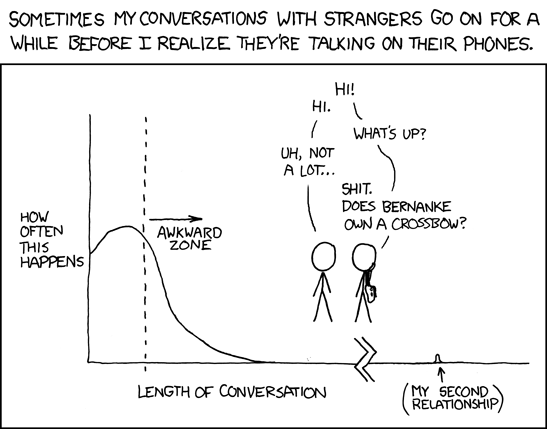
\includegraphics[scale=.55]{comics/476}
\end{center}

\end{multicols}

\clearpage

\subsection{Musterstudienplan für den Studiengang B.Sc.  Wirtschaftsmathematik-
Variante BWL}

\begin{center}
\begin{tabular}{||l||l|l|l|l|l|l||}
\hhline{|t:=:t:=t=t=t=t=t=:t|}
\hspace*{25mm}&1. Semester\hspace*{8ex}&2. Semester\hspace*{8ex}&3. Semester\hspace*{8ex}&4.Semester\hspace*{8ex}&5. Semester\hspace*{8ex}&6. Semester\hspace*{8ex}\\
\hhline{|:=::======:|} Pflichtbereich&Analysis I&Analysis II&Mathematische& Proseminar &Seminar& Bachelorarbeit\\
\hhline{||~||~|~|~|~|~|~||} Mathematik &(9 LP)&(9 LP)&Stochastik&(4 LP) &(6 LP)& (12 LP)\\
\hhline{||~||~|~|~|~|~|~||} &&&(9 LP)&&&\\
\hhline{||~||~|~|~|~|~|~||} &Lineare Algebra&Lineare Algebra&&&&\\
\hhline{||~||~|~|~|~|~|~||} &und Analytische &und Analytische&Numerische& & &\\
\hhline{||~||~|~|~|~|~|~||} &Geometrie I&Geometrie II&Mathematik&&&\\
\hhline{||~||~|~|~|~|~|~||} &(9 LP)&(9 LP)&(9 LP)&&&\\
\hhline{||~||~|~|~|~|~|~||} &&&&&&\\
\hhline{||~||~|~|~|~|~|~||} &&& Informations- &&&\\
\hhline{||~||~|~|~|~|~|~||} &&& veranstaltung zum &&&\\
\hhline{||~||~|~|~|~|~|~||} &&& Studienverlauf &&&\\
\hhline{||~||~|~|~|~|~|~||} &&& (0 LP) &&&\\
\hhline{||~||~|~|~|~|~|~||} &&&&&&\\
\hhline{|:=::======:|} Pflichtbereich&Investition&Finanzierung&&Mikroökonomik&Makroökonomik&\\
\hhline{||~||~|~|~|~|~|~||} Wirtschaft  &  (6 LP)  &(6 LP) &   &(6 LP) &  (6 LP)  &\\
\hhline{||~||~|~|~|~|~|~||} &&&&&&\\
\hhline{|:=::======:|} Vertiefungsbereich&&&&Vertiefungsmodule&Vertiefungsmodule&Vertiefungsmodule \\
\hhline{||~||~|~|~|~|~|~||} Mathematik&&&&(11 LP)&(7 LP)&(9 LP)\\
\hhline{||~||~|~|~|~|~|~||} &&&&&&\\
\hhline{|:=::=|=|=|=|=|=:|} Wahlpflichtbereich&Wahlpflichtmodule&&Wahlpflichtmodule &Wahlpflichtmodule&Vertiefungsmodule&Vertiefungsmodule \\
\hhline{||~||~|~|~|~|~|~||} Wirtschaft&(6 LP)&&(6 LP)&(9 LP)&(6 LP)&(6 LP)\\
\hhline{||~||~|~|~|~|~|~||} &&&&&&\\
\hhline{|:=::======:|} ABK-Bereich&&Programmier-&Softwarepraktikum&&Betriebspraktikum/& \\
\hhline{||~||~|~|~|~|~|~||} &&methoden&(4 LP)&&Projekt/Tutorium&\\
\hhline{||~||~|~|~|~|~|~||} &&(5 LP)&&&(5 LP)&\\
\hhline{||~||~|~|~|~|~|~||} &&&&&&\\
\hhline{|:=::======:|} Wahlbereich&&Wahlmodule&Wahlmodule&&&Wahlmodule\\
\hhline{||~||~|~|~|~|~|~||} &&(1 LP)&(2 LP)&&&(3 LP)\\
\hhline{||~||~|~|~|~|~|~||} &&&&&&\\
\hhline{|b:=:b:======:b|}
\end{tabular}
\end{center}

\clearpage

\subsection{Musterstudienplan für den Studiengang B.Sc.-Wirtschaftsmathematik -Variante VWL}

\begin{center}
\begin{tabular}{||l||l|l|l|l|l|l||}
\hhline{|t:=:t:=t=t=t=t=t=:t|}
\hspace*{25mm}&1. Semester\hspace*{8ex}&2. Semester\hspace*{8ex}&3. Semester\hspace*{8ex}&4.Semester\hspace*{8ex}&5. Semester\hspace*{8ex}&6. Semester\hspace*{8ex}\\
\hhline{|:=::======:|} Pflichtbereich&Analysis I&Analysis II&Mathematische&Proseminar&Seminar&Bachelorarbeit\\
\hhline{||~||~|~|~|~|~|~||} Mathematik &(9 LP)&(9 LP)&Stochastik&(4 LP)&(6 LP)& (12 LP)\\
\hhline{||~||~|~|~|~|~|~||} &&&(9 LP)&&&\\
\hhline{||~||~|~|~|~|~|~||} &Lineare Algebra&Lineare Algebra&&&&\\ 
\hhline{||~||~|~|~|~|~|~||} &und Analytische&und Analytische&Numerische&&&\\ 
\hhline{||~||~|~|~|~|~|~||} &Geometrie I&Geometrie II&Mathematik&&&\\ 
\hhline{||~||~|~|~|~|~|~||} &(9 LP)&(9 LP)&(9 LP)&&&\\
\hhline{||~||~|~|~|~|~|~||} &&&&&&\\
\hhline{||~||~|~|~|~|~|~||} &&& Informations- &&&\\
\hhline{||~||~|~|~|~|~|~||} &&& veranstaltung zum &&&\\
\hhline{||~||~|~|~|~|~|~||} &&& Studienverlauf &&&\\
\hhline{||~||~|~|~|~|~|~||} &&& (0 LP) &&&\\
\hhline{||~||~|~|~|~|~|~||} &&&&&&\\
\hhline{|:=::======:|} Pflichtbereich&Investition&Mikroökonomie&Makroökonomik&Finanzierung&&\\
\hhline{||~||~|~|~|~|~|~||} Wirtschaft&(6 LP)&(6 LP)&(6 LP)&(6 LP)&&\\
\hhline{||~||~|~|~|~|~|~||} &&&&&&\\
\hhline{|:=::======:|} Vertiefungsbereich&&&&Vertiefungsmodule&Vertiefungsmodule&Vertiefungsmodule\\
\hhline{||~||~|~|~|~|~|~||} Mathematik&&&&(11 LP)&(7 LP)&(9 LP)\\
\hhline{||~||~|~|~|~|~|~||} &&&&&&\\
\hhline{|:=::======:|} Wahlpflichtbereich&Wahlpflichtmodule&&&Wahlpflichtmodule&Wahlpflichtmodule&\\
\hhline{||~||~|~|~|~|~|~||} Wirtschaft&(6 LP)&&&(9 LP)&(6 LP)&\\
\hhline{||~||~|~|~|~|~|~||} &&&&&&\\
\hhline{||~||~|~|~|~|~|~||} &&&&&Vertiefungsmodule&Vertiefungsmodule\\
\hhline{||~||~|~|~|~|~|~||} &&&&&(6 LP)&(6 LP)\\
\hhline{||~||~|~|~|~|~|~||} &&&&&&\\
\hhline{|:=::======:|} ABK-Bereich&&Programmier-&Softwarepraktikum&&Betriebspraktikum/&\\
\hhline{||~||~|~|~|~|~|~||} &&methoden&(4 LP)&&Projekt/Tutorium&\\
\hhline{||~||~|~|~|~|~|~||} &&(5 LP)&&&(5 LP)&\\
\hhline{||~||~|~|~|~|~|~||} &&&&&&\\
\hhline{|:=::======:|} Wahlbereich&&Wahlmodule&Wahlmodule&&&Wahlmodule\\
\hhline{||~||~|~|~|~|~|~||} &&(1 LP)&(2 LP)&&&(3 LP)\\
\hhline{||~||~|~|~|~|~|~||} &&&&&&\\
\hhline{|b:=:b:======:b|}
\end{tabular}
\end{center}
\clearpage

\begin{multicols}{2}
\section{Lehramt Primarstufe und Sekundarstufe I und Lehramt an der
Sonderschule}

Hier nun ein paar grundlegende Informationen für Studierende des Lehramts der
Primar- und Sekundarstufe I und des Lehramts der Sonderschule: Auch nach der
Umstellung auf Bachelor- und Master-Studiengänge gibt es für Euch einen eigenen
Studiengang, der weitestgehend losgelöst von den Bachelor- und anderen
Lehramts-Studierenden ist. Im ersten Studienabschnitt, dem Bachelor, müsst ihr
im Pflichtbereich insgesamt sieben Module absolvieren, also insgesamt 45 LP.
Diese Module sind: \emphm{Grundlagen der Mathematik} (M1), \emphm{Grundbildung
Lineare Algebra} (M2), \emphm{Grundbildung Analysis} (M3) (je 4 SWS Vorlesungen
und 2 SWS Übungen, 9 LP), \emphm{Grundbildung Geometrie} (GG),
\emphm{Grundbildung Stochastik} (GS) (je 2+1 SWS, 5 LP) und ein
\emphm{Softwarepraktikum} (EMS) (2 SWS, 4 LP). Außerdem müsst ihr ein
\emph{Proseminar} (PSEM) belegen (2 SWS, 4 LP). Um GG, EMS, GS und PSEM belegen
zu dürfen, muss M1 erfolgreich abgeschlossen sein.

Jede Woche gibt es Übungen, die aufgeteilt sind in einen Präsenz- und einen
Hausaufgabenteil. Im Präsenzteil werden mit einem Dozenten Aufgaben gerechnet
und besprochen. Im Hausaufgabenteil werden die Aufgaben besprochen, die vorher
bereits in Zweier- bis Dreiergruppen angefertigt und abgegeben wurden.  Um an
der Klausur teilnehmen zu dürfen, müssen in den Hausaufgaben 50\% der möglichen
Punkte erreicht werden und pro Student einmal eine Aufgabe an der Tafel
vorgerechnet werden. Jedes Modul wird jedes zweite Semester angeboten, also
entweder im Winter- oder im Sommersemester. Am Ende eines Semesters werden zwei
Prüfungstermine angeboten, insgesamt dürfen maximal vier Versuche erfolgen.
Achtung: Hier sind die Referenzsemester wichtig!

Das Masterstudium ist gegliedert in einen Vertiefungsbereich, einen
Projektbereich und für Lehrämtler Primar- und Sekundarstufe zusätzlich einen
Wahlbereich. Im Vertiefungsbereich sind Module im Gesamtumfang von (mindestens)
10 LP, im Projektbereich Module im Gesamtumfang von (mindestens) 5 LP und im
Wahlbereich für LAPS (mindestens) 5 LP zu absolvieren. 

\begin{center}
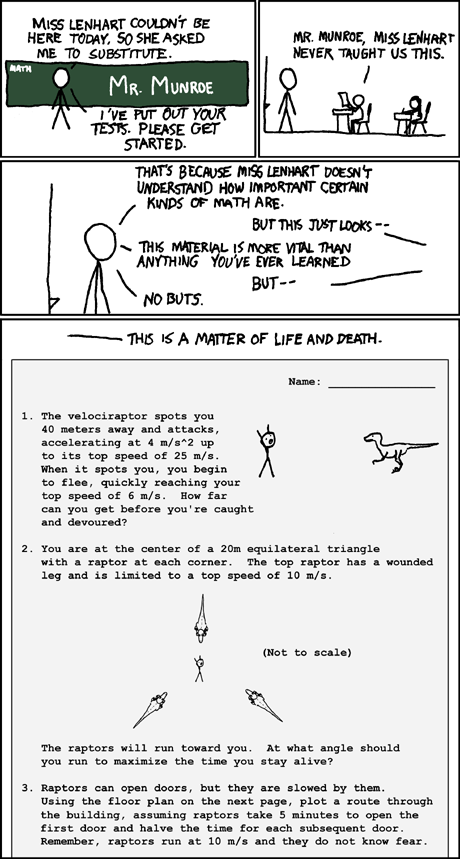
\includegraphics[scale=.57]{comics/135}
\end{center}

\end{multicols}
\subsection{Musterstudienplan für den Studiengang Lehramt Primarstufe und
Sekundarstufe I und Lehramt an der Sonderschule} 

% TODO: Anpassen
\begin{center}
\begin{tabular}{||l||l|l|l|l|l||}
\hhline{|t:=:t:=====:t|} Semester\hspace*{4mm}
    &Kürzel
    &Module\hspace*{5ex}
    &SWS\hspace*{6ex}
    &LP\hspace*{4ex}
    &Referenzsemester\hspace*{4ex} \\
\hhline{||=::=====||} 1&M1&Grundlagen der Mathematik&4+2&9&3\\
\hhline{||~||~|~|~|~|~||} &&&&&\\
\hhline{||=::=====||} 2&M2&Grundbildung Lineare Algebra und Analytische Geometrie&4+2&9&4\\
\hhline{||~||~|~|~|~|~||} &&&&&\\
\hhline{||=::=====||} 3&M3&Grundbildung Analysis&4+2&9&5\\
\hhline{||~||~|~|~|~|~||} &&&&&\\
\hhline{||=::=====||} 4&GG&Grundbildung Geometrie&2+1&5&6\\
\hhline{||~||~|~|~|~|~||} &&&&&\\
\hhline{||~||~|~|~|~|~||} &EMS&Einführung in mathematische Software&2&4&6\\
\hhline{||~||~|~|~|~|~||} &&&&&\\
\hhline{||=::=====||} 5&GS&Grundbildung Stochastik&2+1&5&6\\
\hhline{||~||~|~|~|~|~||} &&&&&\\
\hhline{||=::=====||} 6&PSEM&Proseminar&2&4&6\\
\hhline{||~||~|~|~|~|~||} &&&&&\\
\hhline{|b:=:b:=====:b|}
\end{tabular}
\end{center}
\clearpage

\begin{multicols}{2}[\section{Lehramt an Gymnasien}]

Am Fachbereich Mathematik solltest du -- zusammen mit den anderen
Mathematik-StuStudenten -- dein Studium mit Modulen aus dem
veranstaltungsgebundenen Pflichtbereich beginnen. Die Module \emphm{Analysis}
und \emphm{Lineare Algebra \& Analytische Geometrie}, welche aus den
Veranstaltungen \emphm{Analysis I} und \emphm{II} bzw. \emphm{Lineare Algebra
\& Analytische Geometrie I} und \emphm{II} bestehen, müssen im Pflichtbereich
absolviert werden. Ebenso ein \emphm{Softwarepraktikum} (SW).

Mit \emphm{Lineare Algebra \& Analytische Geometrie I} (LAAG-I) fängst du
dieses Semester schon an. Im zweiten Semester belegst du dann \emphm{Lineare
Algebra \& Analytische Geometrie II} (LAAG-II). Im dritten und vierten Semester
folgen \emphm{Analysis I} (ANA-I) und \emphm{Analysis II} (ANA-II). Die
Veranstaltungen bestehen jeweils aus 4 SWS Vorlesung, 2 SWS Übung und
freiwilligen Tutorien. Zum Ende des (zweiten bzw. vierten) Semesters schließt
du das jeweilige Modul mit einer benoteten Modulprüfung (das kann eine Klausur
oder mündliche Prüfung sein) ab.

Das unbenotete Softwarepraktikum, das 2 SWS einschließt, musst du erst während
des Masterstudiums belegen. 

Aus dem Gebiet des \emph{veranstaltungsgebundenen Pflichtbereichs} musst du
drei \emph{lehramtsspezifische Veranstaltungen} belegen, sowie ein
\emphm{Seminar} (2 SWS).  Du belegst im zweiten Semester die erste
Lehramtsspezifische Veranstaltung (LSV, Typ I) und im dritten die zweite (LSV,
Typ II).  Das Seminar (SEM) ist für das vierte Semester vorgesehen.

Je nachdem, ob Mathematik dein erstes oder dein zweites Unterrichtsfach ist,
wirst du während deines Bachelor- (wenn erstes Fach) oder während deines
Masterstudiums (wenn zweites Fach) ein \emph{Lehramtsspezifisches Projekt}
(PROJ) über 1 LP modulbegleitend absolvieren.

Im Wahlpflichtbereich wirst du vier Module (A, B, C, D) absolvieren müssen.
Davon sollten eines eine 6 LP Veranstaltung und drei 9 LP Veranstaltungen sein.
Die vier Module müssen aus dem Wahlpflichtangebot des Bachelor
Mathematik-Studienganges sein, zuzüglich der Module \emphm{Höhere Analysis},
\emphm{Numerische Mathematik} und \emphm{Mathematische Stochastik}. Wenn
Mathematik dein erstes Unterrichtsfach ist, wirst du drei dieser vier Module in
den letzten Semestern deines Bachelorstudienganges absolvieren müssen, und nur
noch eines im Masterstudium.  Ist hingegen Mathematik dein zweites
Unterrichtsfach, dann belegst du zwei der vier Module während des Bachelor- und
zwei während des Masterstudiums. Um diese Module wählen zu können, musst du in
STiNE unter Fächer/Bereichswahl die jeweiligen Gebiete auswählen. Sonst bietet
STiNE sie dir nicht zur Wahl an. Dasselbe gilt für die lehramtsspezifischen
Veranstaltungen: Die Auswahl wird sehr viel größer.

Außerdem musst du mit den Modulen A,B,C und D, den lehramtsspezifischen
Veranstaltungen und dem Seminar insgesamt 2 der Bereiche \emph{Reine
Mathematik}, \emph{Angewandte Mathematik} und \emph{Stochastik} abdecken, wenn
Mathematik dein erstes Unterrichtsfach ist. Ist Mathematik dein zweites Fach,
musst du nur einen Bereich abdecken. Im Bachelor und Master müssen alle drei
Bereiche abgedeckt werden. Im Master musst du außerdem begleitend zu einem der
Module (B,C,D) ein \emph{Lehramtsspezifisches Referat} (REF) über 2 LP halten.

\begin{center}
\vfill
\includegraphics[scale=.9]{comics/552}
\end{center}

\clearpage
\end{multicols}
\subsection{Musterstudienplan für Lehramt Gymnasium (Bachelor und Master)}

\begin{center}
\begin{tabular}{|p{13mm}|p{40mm}||p{40mm}|p{40mm}|p{40mm}|}
\hline 				Sem. & 1.Fach Mathe & 2.Fach Mathe & SWS & LP \\
\hhline{|=|=|=|=|=|} 1.  & LAAG-I 	  & LAAG-I  	  & 6   & 9  \\
                         &            &              &     &    \\
\hline				 2.	 & LAAG-II	  & LAAG-II	 	  & 6	  & 9  \\
						       & LSV-I		  & LSV-I	     & 2	  & 3  \\
\hline				 3.	 & ANA-I		  & ANA-I	 	  & 6	  & 9  \\
						       & LSV-II     & LSV-II	     & 2   & 3  \\
\hline				 4.	 & ANA-II	  & ANA-II 	     & 6	  & 9  \\
						       & SEM  		  & SEM			  & 2	  & 3  \\
\hline				 5.	 & A		     & A	           & 6	  & 9  \\
						       & B oder D	  & B oder D	  & 4	  & 6  \\
\hline				 6.	 & D oder B	  & 	           & 6	  & 9  \\
						       & + PROJ	  & 	 	        & 	  & +1 \\
\hhline{|=|=|=|=|=|} 7.  & SW			  & SW 			  & 2	  & 4  \\
						       & 			  & 			     & 	  &    \\
\hline 				 8.    & 			  & D oder B 	  & 6	  & 9  \\
						       & 			  & + PROJ 		  & 	  & +1 \\
\hline				 9.    & C			  &              & 6	  & 9  \\
						       & + REF		  &    	        & 	  & +2 \\
\hline				 10.   & 			  & C 		     & 6   & 9  \\
                         &            & + REF        &     & +2 \\
\hline
\end{tabular}

\end{center}
\clearpage

\begin{multicols}{2}[\section{Lehramt Berufsschule}]

Da sich die einzelnen Module deines Studiengangs nicht von denen des
Studiengangs Lehramt am Gymnasium unterscheiden, können die Modulbeschreibungen
aus dem entsprechenden Artikel übernommen werden.

Auch der \emph{veranstaltungsungebundene Pflichtbereich} ist identisch zum
Lehramt Gymnasium (LAG) und besteht somit aus den Modulen \emphm{Analysis},
\emphm{Lineare Algebra und analytische Geometrie} und einem
\emphm{Softwarepraktikum}. Da ihr allerdings im Laufe eures Studiums weniger
Veranstaltungen abdecken müsst als die Studierenden des LAG, empfehlen wir euch
in den ersten beiden Semestern \emphm{Lineare Algebra und analytische Geometrie
I+II} (LA 1+2) zu hören und erst im dritten und vierten Semester
\emphm{Analysis I+II} (Ana 1+2) zu belegen. Wie die LAG-Studenten auch musst du
das \emphm{Softwarepraktikum} (SW) erst während des Masterstudiums belegen. Wir
empfehlen dir, dieses im siebten Semester zu tun.

Auch du musst zwei \emph{lehramtsspezifische Veranstaltungen} (LSV-I,II)
belegen, beide davon während deines Bachelorstudiums und empfohlen wird das
fünfte Semester. Das letzte veranstaltungsgebundene Pflichtmodul besteht auch
bei euch aus einem \emphm{Seminar} (SEM).

Im \emph{Wahlpflichtbereich} musst du nur ein Modul belegen, welches aus dem
Wahlpflichtangebot des Bachelor Mathematik-Studienganges oder aus den Modulen
\emphm{Höhere Analysis}, \emphm{Numerische Mathematik} und \emphm{Mathematische
Stochastik} stammen sollte. Du musst allerdings beachten, dass du mit diesem
Modul und dem veranstaltungsgebundenen Pflichtbereich insgesamt zwei der drei
Bereiche \emph{Stochastik}, \emph{Angewandte Mathematik} und \emph{Reine
Mathematik} abdeckst. Das Modul mit dem Wahlpflichtbereich musst du erst
während des Masterstudiums belegen, empfohlen wird hierfür das achte Semester.
Begleitend zu diesem Modul musst du wie die LAG-Studenten noch ein
lehramtsspezifisches Referat (REF) über zwei Leistungspunkte halten.

\end{multicols}
\begin{center}

\includegraphics[scale=7]{comics/263}
\end{center}
\begin{multicols}{2}

\end{multicols}
\clearpage
\subsection{Musterstudienplan für den Studiengang Lehramt Berufliche Schulen}

\begin{center}
\begin{tabular}{||p{21mm}||p{20mm}|p{20mm}|p{20mm}|p{20mm}|p{20mm}|p{20mm}||p{20mm}|p{20mm}|p{20mm}||}

\hhline{||=||=|=|=|=|=|=||=|=|=||}& 1.Sem & 2. Sem & 3. Sem & 4. Sem & 5. Sem & 6 Sem. & 7. Sem & 8. Sem & 9./10. Sem \\ 
\hline							 gebundene& Lineare & Lineare & Analysis I & Analysis II &  &&Software-&&\\
								 Pflicht-& Algebra I & Algebra II &  & &  &&Praktikum&&\\
								 module& (9LP) & (9LP) & (9LP)& (9LP) &  &&(4LP)&&\\
\hhline{||=||=|=|=|=|=|=||=|=|=||} ungebundene& & &&& LSV, & Seminar &  &&\\
								   Pflicht-	  & & &&& Typ I& & &&\\
								   module     & & &&& (3LP)   & (3LP)   & &&\\
							   &&&&&&&&&\\
							   &&&&& LSV,&&&&\\
							   &&&&& Typ II&&&&\\
							   &&&&& (3LP) &&&&\\
\hhline{||=||=|=|=|=|=|=||=|=|=||} Wahlpflicht-&&&&&&&&Modul&\\
							   module&&&&&&&&+ Referat&\\
							   &&&&&&&& (9+2 LP)&\\
\hline						
\end{tabular}
\end{center}

\begin{multicols}{2}

\end{multicols}

\section{Was ist STiNE?}
\begin{multicols}{2}
Das Studien-Infonetz der Universität Hamburg, STiNE, ist ein internetbasiertes
Informations- und Kommunikationssystem für Studium und Lehre. Dieses System
wurde eingeführt, um den Alltag an der Universität leichter zu machen. Mithilfe
dieses Online-Portals kann der Student an der Universität Hamburg seine
Vorlesungen verwalten, sich für Prüfungen an- und abmelden und seine Noten in
einer übersichtlichen Form abrufen.

Derzeit werden die an der Universität Hamburg angebotenen Studiengänge im
Rahmen des \emph{Bologna-Prozesses} auf das Bachelor- und Masterstudiensystem
umgestellt. Im Zuge der Umstellung werden in den neuen Studiengängen Module
eingeführt, die mit einem internationalen Leistungspunktesystem bewertet
werden. Das Bachelorstudium wird nicht durch eine große Abschlussprüfung
beendet, sondern jedes Modul schließt mit einer Prüfung ab, die automatisch zu
einem Teil in die Note des Bachelors eingeht. Mit STiNE kann man sich über die
jeweiligen Prüfungsordnungen in den Bachelorstudiengängen informieren.
Gleichzeitig gibt es die Möglichkeit, den aktuellen Stand seines
Leistungspunktekontos abzufragen und sich über Ergebnisse seiner absolvierten
Prüfungen zu informieren.

Die Bestimmungen zum Datenschutz bei STiNE sind sehr streng. Keiner der
Dozenten kann die alten Prüfungsergebnisse seiner Studenten einsehen. Nur dem
Student selber und dem Prüfungsamt ist dieses erlaubt. Eine Note kann nur mit
erheblichem Aufwand geändert werden.

Bei der Anmeldung zu einer Vorlesung muss man sich in der Regel gleich zur
Prüfung mit anmelden. Hierzu benötigt man jeweils eine \emph{indizierte
Transaktionsnummer} (iTAN) aus seiner persönlichen Tanliste. Diese sollte
spätestens erneuert werden, wenn nur noch zwei iTANs übrig sind, da man eine
für die Beantragung einer neuen Liste und eine für die Freischaltung ebendieser
benötigt.  Innerhalb der Anmeldefrist können Anmeldungen jederzeit storniert
werden. Auch nach der Zuteilung eines Teilnehmerplatzes ist eine Stornierung
noch innerhalb von zwei Wochen nach Ablauf der Anmeldefrist möglich.

Bei der Eingabe des automatisch generiertem Passworts sollte man beachten, dass
bei dem Bogen für die Anmeldedaten eine Standardschrift verwendet wird, die es
unter Umständen erschwert das Kennwort eindeutig zu identifizieren. So ähneln
sich die Null und das große O sowie die Eins, das kleine L und das große i. Um
die Sicherheit seiner Daten zu bewahren sollte man das Passwort gleich nach dem
ersten Anmelden ändern. Hierbei solltest du ein ausreichend sicheres Passwort
verwenden.

Eine weitere nützliche Option bei STiNE ist der Terminexport, der es einem
ermöglicht die Termine einer Woche in einer Datei zu speichern und diese in
einen elektronischen Terminkalender zu importieren. Von dort aus können die
Termine mit dem Handy synchronisieren werden. Mit dieser technischen Spielerei
hat man ganz leicht seine Vorlesungen und Veranstaltungen im Überblick.

\begin{center}
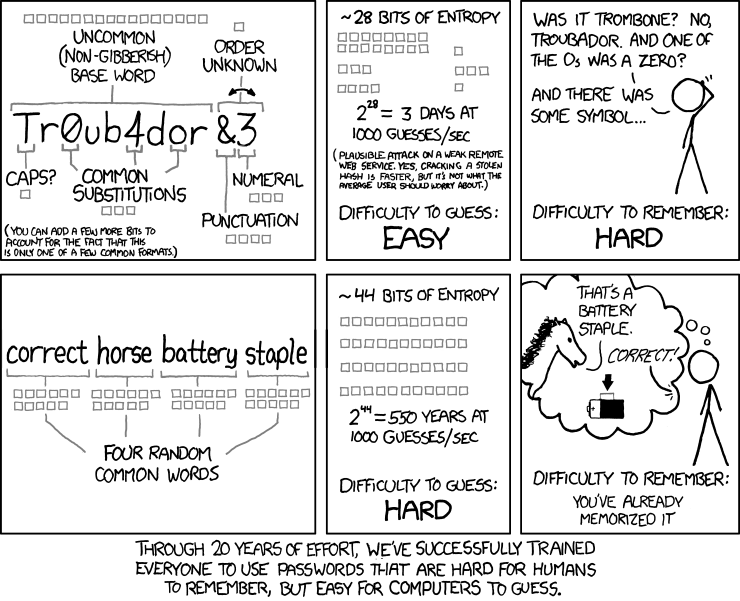
\includegraphics[scale=0.5725]{comics/936}
\end{center}

\end{multicols}

\section{Eure Professoren stellen sich vor}
\begin{multicols}{2}
\subsection{Grundlagen der Mathematik f\"ur Studierende der Lehr\"amter
Primar- und Sekundarstufe I sowie Sonderschulen} 

Mein Studium begann ich 1979 an der TU M\"unchen, und schloss 1986 mit dem
ersten Staatsexamen f\"ur das Lehramt an Gymnasien in den F\"achern Mathematik
und Physik ab. Nach Stationen in M\"unchen, Tucson (Arizona), und wieder
M\"unchen, kam ich 1999 nach Hamburg.

Die solide mathematische Ausbildung von Studierenden des Lehramts liegt mir
besonders am Herzen.  Sie werden sehen, dass Mathematik Spa\ss{} machen kann.
Wenn Sie eine zun\"achst unl\"osbar scheinende Aufgabe schlie"slich doch
herausbekommen, k\"onnen Sie ein tiefe Befriedigung erleben.  Freilich setzt
das ausdauerndes, kontinuierliches Arbeiten und fundierte Kenntnisse der
Schulmathemetik voraus. Die Sch\"onheit der Mathematik erschlie"st sich nur den
Personsn, die sich intensiv darum bem\"uhen.

Inhaltlich wird es im ersten Semester um Grundlagen gehen, wie etwa
\textit{Mengen, Logik, Relationen, Funktionen, vollst\"andige Induktion, Aufbau
des Zahlensystems,} uvam.

Ich freue mich darauf Ihnen in den kommenden Semestern die Sch\"onheit der
Mathematik nahebringen zu d\"urfen und hoffe auf eine gute Zusammenarbeit.  Bis
dahin w\"unsche ich Ihnen eine interessante und abwechslungsreiche OE. Nutzen
Sie die Zeit, Kommilitonen auch anderer Studienrichtungen kennen zu lernen.

Viel Erfolg in Ihrem ersten Semester!

\bigskip

\hfill Hubert Kiechle

Hubert Kiechle\\
Bereich Geometrie\\
Fachbereich Mathematik\\
\Telefon\ 42~83~8 - 51~86, Raum 224\\
\Letter\ \href{mailto:hubert.kiechle@uni-hamburg.de}{hubert.kiechle@uni-hamburg.de}\\
\url{http://www.math.uni-hamburg.de/home/kiechle/}

\subsection{Analysis}

Ihr Mathematikstudium beginnt mit den Veranstaltungszyklen \glqq Lineare
Algebra\grqq\ und \glqq Analysis\grqq. Eine solche Aufteilung wird seit vielen
Jahrzehnten weltweit an fast allen Universit\"aten praktiziert und hat sich
bew\"ahrt. Diese Vorlesungen bilden die Grundlage f\"ur alle weiteren
Veranstaltungen Ihres Studiums.

W\"ahrend bei der linearen Algebra neben grundlegenden algebraischen Strukturen
das lineare Gleichungssystem im Vordergrund steht, geht es in meiner
Veranstaltung \glqq Analysis\grqq\ eher um sogenannte \glqq topologische
Aspekte\grqq. D.h., es geht um Fragestellungen, die damit zusammenh\"angen, ob
Zahlen (oder auch Vektoren o.\"A.) \glqq nahe beieinanderliegen\grqq. Die
daraus herleitbaren Begriffe wie Konvergenz, Grenzwert, Stetigkeit,
Differenzierbarkeit und Integrale sind gleichwohl zentrale Konzepte der
Analysis und werden in dieser Veranstaltung behandelt. Diese Begriffe kommen
Ihnen sicherlich bekannt vor; wir werden sie jedoch von Grund auf neu
einf\"uhren.  Anders als vielleicht in der Schule stehen
Universit\"atsvorlesungen eher axiomatische Zug\"ange im Vordergrund.  Das
macht Anf\"angern erfahrungsgem\"a\ss\ h\"aufig Schwierigkeiten. Diese k\"onnen
Sie \"uberwinden, indem Sie beharrlich \glqq am Ball bleiben\grqq: Dazu
geh\"ort etwa das Bearbeiten von \"Ubungsbl\"attern und die regelm\"a\ss ige
Nachbearbeitung des Vorlesungsstoffs. Bei Letzterem werden wir Sie in Form der
Anbietung sogenannter \glqq Tutorien\grqq\ unterst\"utzen; dort k\"onnen Sie
beispielsweise Fragen zum Vorlesungsinhalt und darüber hinaus stellen, welche
meine Mitarbeiter und ich Ihnen gerne beantworten wollen.

Dass die mathematische Welt strikt und disjunkt in Analysis und lineare Algebra
aufgeteilt ist, wird bereits in Ihrem zweiten Semester widerlegt. Dort werden
wir, wenn wir in \glqq Analysis II\grqq\ Funktionen mit mehreren
Ver\"anderlichen betrachte, auch auf Konzepte der linearen Algebra zugreifen,
wie etwa Matrizen.  In Ihrem weiteren Studium werden Sie sehen, dass sich die
Inhalte beider Veranstaltungen immer mehr ineinander verzahnen. Mein Interesse
besteht darin, dass sie m\"oglichst viel aus der Analysis lernen und dass Sie
im Rahmen meiner Vorlesung ebenfalls einen gewissen Gesamteindruck der
Mathematik bekommen, um Ihnen somit eine gute Grundlage f\"ur ein erfolgreiches
Mathematikstudium zu erm\"oglichen.

\clearpage

Ich selbst arbeite in meiner mathematischen Forschung an Steuerungs-,\linebreak
Regelungs- und Approximationsproblemen bei Differentialgleichungen und
besch\"aftige mich insbesondere mit Anwendungen in der Elektrotechnik. Im Jahr
1998 begann ich in Kaiserslautern mit dem Studium der Mathematik und ging nach
meiner Promotion 2006 als wissenschaftlicher Mitarbeiter an die Technische
Universit\"at Berlin. Nach einem jeweils etwa einj\"ahrigen Engagement als
Gastwissenschaftler an der Rice University in Houston/Texas und als
Vertretungsprofessor an der Technischen Universit\"at Hamburg-Harburg nahm ich
im vergangenen Jahr 2011 einen Ruf auf eine Professur an der Universit\"at
Hamburg an.

Ich freue mich, dass man meinem Wunsch nach dem Halten einer
Anf\"angervorlesung f\"ur Mathematikstudenten entsprochen hat und hoffe auf
angenehme und erfolgreiche Zusammenarbeit mit Ihnen.

Ich w\"unsche Ihnen einen angenehmen Einstieg ins Studium und viel Erfolg!

\bigskip

\hfill Timo Reis

Prof.~Dr.~Timo Reis\\
Bereich Optimierung und Approximation\\
Fachbereich Mathematik\\
\Telefon\ 42~83~8 - 51~11, Raum 123\\
\Letter\ \href{mailto:timo.reis@math.uni-hamburg.de}{timo.reis@math.uni-hamburg.de}\\
\url{http://www.math.uni-hamburg.de/home/reis}


%\documentclass{amsart}
%\usepackage{amssymb}

\subsection{Lineare Algebra \& Analytische Geometrie}

Mathematik habe ich an der Universit\"at Bonn studiert und dort auch 2000
promoviert. W\"ahrend meiner Assistentenzeit war ich bei l\"angeren
Forschungsaufent\-halten in Stra{\ss}burg und Oslo. Seit 2005 bin ich
Professorin f\"ur Algebraische Topologie in Hamburg. Meine
Forschungsschwerpunkte liegen in der stabilen Homoto\-pie\-theorie und der
homologischen Algebra.

\phantom{Die Lehre liegt mir sehr am Herzen und ich freue mich darauf, Ihnen in der}
Die Lehre liegt mir sehr am Herzen und ich freue mich darauf, Ihnen in der
Vorlesung \emph{Lineare Algebra und analytische Geometrie} einen ersten
Einblick in die faszinierende Welt der Mathematik geben zu k\"onnen!

Die Lineare Algebra, wie auch die Analysis, geh\"ort zu den Grundlagen eines
jeden Mathematikstudiums. Die Inhalte dieser Vorlesung werden Sie in Ihrem
weiteren Studium brauchen. Dar\"uberhinaus erlernen Sie in den Grundvorlesungen
die Arbeitsmethoden, die Sie als Mathematiker und Mathematikerin ben\"otigen,
sei es in der Schule, in der Wirtschaft oder in der Forschung. 

Mathematik lernt man, indem man selbst Mathematik macht. Seien Sie aktiv und
verfallen Sie in den Vorlesungen bitte nicht in eine Konsumhaltung!  Nur das,
was Sie sich selbst angeeignet haben, verstehen Sie auch. Bleiben Sie
neugierig! Wir bieten Ihnen \"Ubungsaufgaben an, um Ihnen bei der
Auseinandersetzung mit dem Stoff der Vorlesungen zu helfen. Aufgaben zu
bearbeiten ist zwar anstrengend, aber es lohnt sich.  Mathematik macht
gl\"ucklich: Wenn Sie lange an einem Problem geknobelt haben und Sie haben es
schlie{\ss}lich verstanden, dann ist das ein gutes Gef\"uhl. 

Nutzen Sie bitte die Angebote, die wir bieten. Wenn Sie unvorbereitet in die
\"Ubungsgruppen gehen, werden Sie kaum etwas mitnehmen. Wenn Sie die Vorlesung
nacharbeiten, werden Sie sicherlich Fragen haben. Stellen Sie diese in den
\"Ubungsgruppen und in den Tutorien. Haken Sie solange nach, bis Sie alles
verstanden haben! 

Ich hoffe, Ihnen gelingt die Umstellung von der Schule auf die Universit\"at
und von der Schulmathematik auf Mathematik.   F\"ur Ihren Studienbeginn
w\"unsche ich Ihnen viel Erfolg und alles Gute!

\bigskip

\hfill Birgit Richter

Birgit Richter \\
Bereich Algebra und Zahlentheorie\\
Fachbereich Mathematik\\
\Telefon\ 42~83~8 - 51~73, 42~83~8 - 51~71 (Sekretariat) \\
\Letter\ birgit.richter@uni-hamburg.de\\
\url{http://www.math.uni-hamburg.de/home/richter/}

\end{multicols}

\section{Fahrplan}
\begin{tabularx}{1.005\textwidth}{||X|X||X|X|X|X|X||}
\hhline{|t:=======:t|} \centering{Donnerstag}
& \centering{Freitag}
& \centering{Montag}
& \centering{Dienstag}
& \centering{Mittwoch}
& \centering{Donnerstag}
& Freitag, Samstag \\
\centering{4.10}
& \centering{5.10}
& \centering{8.10}
& \centering{9.10}
& \centering{10.10}
& \centering{11.10}
& \hspace{4.5ex} 13+14.10 \\ % centering funktioniert hier nicht. Warum?
&&&&&&\\
\hhline{|:==::=====:|} Begrüßung\newline 9:30 Geom H1
& AG I\newline 9:00 Geom $\diamondsuit$
& Studienberatung\newline 9:00 Geom $\clubsuit$ %Professoren und \makebox{STiNE}\newline 9:00 Geom H1
& 
& SIV\newline 9:00 Geom H2
& Mathematik und Gesellschaft\newline 9:30 Geom H4
& Abschlussfahrt\newline 8:30 Foyer \\
&&&&&&\\
\hhline{||--||----~||} Kennenlernen\newline 10:30 Geom $\clubsuit$
& Tutorium\newline 11:00 Geom $\spadesuit$ %AG I\newline 11:00 Geom $\diamondsuit$
& Q.E.D. II\newline 11:30 Geom $\spadesuit$
& Ergänzungsfächer, Campus-Tour\newline 11:00 Geom H2%Vorbereitung der Abschlussfahrt\newline 12:00 Geom H2
& Übungsgruppe\newline 11:00 Geom $\spadesuit$%Ergänzungsfächer, Campus-Tour\newline 11:00 Geom H2
& Erasmus-Vorstellung\newline 12:00 Geom H5
& \\
&&&&&&\\
\hhline{||------~||} \multicolumn{6}{||c|}{} & \\
\hhline{||~~~~~~||} \multicolumn{6}{||c|}{Pause} & \\
\hhline{||~~~~~~||} \multicolumn{6}{||c|}{} & \\
\hhline{||------~||} Probevorlesung\newline 13:30 Geom H1%Q.E.D. I\newline 14:00 Geom $\spadesuit$%Studienberatung\newline 13:00 Geom $\clubsuit$
& Q.E.D. I\newline 13:00 Geom $\spadesuit$ %Tutorium\newline 13:00 Geom $\spadesuit$
& Vorbereitung der Abschlussfahrt\newline 14:00 Geom H2%Mathematik im Beruf\newline 13:30 Geom H2
& Mathematik im Beruf\newline 13:30 Geom H2
& Mathematik im Beruf\newline 14:00 Geom H2
& Mathematik im Beruf\newline 13:30 Geom H2
& \\
&&&&&&\\
\hhline{||--||----~||} Rallye\newline 15:30 Foyer
& AG II\newline 15:30 Geom $\spadesuit$%Spieleabend\newline 17:00 Geom R241
& Professoren und \makebox{STiNE}\newline 15:00 Geom H1%AG II\newline 14:15 Geom $\spadesuit$
& %Stadtführung\newline 15:30 Foyer
& Spieleabend\newline im Anschluss\newline Geom R241
& Stadtführung\newline 15:30 Foyer%Übungsgruppe\newline 15:30 Geom $\spadesuit$
& \\
&&&&&&\\
\hhline{||--||--~-~||} Ausklang\newline 17:30 Geo
& Kieztour \newline 21:00 Foyer
& Party\newline20:00 Foyer
&
&
&
& \\
&&&&&&\\
\hhline{|b:=======:b|}
\end{tabularx}


\section{Q.E.D.}
\begin{multicols}{2}
\subsection{Wie bearbeite ich ein Übungsblatt?}

Übungsaufgaben spielen in der Mathamatik eine zentrale Rolle. Mathematik lernt
man nicht nur aus Büchern und durch Besuchen von Vorlesungen, sondern auch
wesentlich durch Selbermachen. Genau dazu geben die Übungen zu den Vorlesungen
Gelegenheit.

\subsubsection{Bearbeitungszeitraum}

In der Regel vergeht zwischen Ausgabe- und Abgabetermin eines Übungsblattes
eine Woche. Das bedeutet, ihr habt eine Woche Zeit zum Nachdenken, Grübeln,
Schmirgeln und Feilen. Diese Zeit müsst ihr vom ersten Augenblick an nutzen.
Nur wenige Aufgaben sind so angelegt, dass sie einfach abgearbeitet werden
können. Manche Aufgaben wird man mechanisch lösen können, etwa solche, die ein
bestimmtes Rechenverfahren einüben sollen. Doch die meisten Aufgaben erwarten,
dass ihr über die Lösung nachdenkt und verschiedene Ansätze ausprobiert.

\subsubsection{Analyse der Aufgabenstellung}

Als Erstes müsst ihr euch aller in der Aufgabenstellung verwendeten Begriffe
versichern. Wiederholt also gegebenenfalls die Definitionen relevanten
Fachwörter. Ihr müsst in jedem Fall sicherstellen, dass ihr mit diesen
Begriffen nicht nur verschwommene Vorstellungen verbindet, sondern ihre präzise
Bedeutung. Die Anschauung, die ein Begriff mit sich bringt, wird häufig erst
durch die Menge aller Sätze gegeben, die über diesen Begriff gemacht werden.
Welche Eigenschaften besitzen die Begriffe? Und in welcher Beziehung stehen sie
zueinander?

\subsubsection{Redet über die Aufgaben!}

Grundsätzlich gilt: Möglichst viel über Mathematik reden. Zu reden hilft, die
eigenen Gedanken zu ordnen. Wenn ihr eine Lösung jemand anderes erklärt und
euch dabei Worte fehlen, oder wenn ein \glqq Na ja, irgendwie so\dots\grqq\
herausrutscht, dann ist das ein Hinweis darauf, dass im Verständnis noch eine
Lücke ist.

\subsubsection{Der Moment des Aufschreibens}

Bei den Abgaben gibt es zwei Extreme, die beide wenig zufriedenstellend sind:
das eine ist eine ganze Seite voller Formeln ohne kommentierenden Text, das
andere Extrem ist der Roman, der um das Problem herumredet. Der eigentliche
Gegenstand der Argumentation werden gewisse definierte Objekte sein und
logische oder mathematische Beziehungen zwischen diesen. Der umgangssprachliche
Text hat die Aufgabe den logischen Stellenwert dieser mathematischen Bausteine
zu klären. Dieselbe mathematische Phrase, z.B. $a<b$ hat ganz unterschiedliche
Bedeutungen je nachdem ob im Text vorher steht: \glqq Hieraus schließen wir,
dass\dots\grqq\ oder \glqq Angenommen, es gilt\dots\grqq. Der Text soll aus
ganzen Sätzen bestehen. Jeder Satz enthält ein Subjekt, ein Prädikat und einen
Punkt am Satzende. Hierbei sind auch Vorlesungen nicht immer Vorbild! Nach dem
Aufschreiben der Lösung solltet ihr den Text noch einmal unter folgendem
Gesichtspunkt durchlesen: Überzeugt die Argumentation des Textes tatsächlich?
Ganz ehrlich? Schließlich sollt ihr nicht einem wissenden Leser durch obskure
Hinweise davon überzeugen, dass ihr auch die Lösung verstanden habt, sondern
ihr sollt so schreiben, dass ein unwissender Leser die Lösung verteht und keine
Fragen offenbleiben.

Weitere Informationen zu diesem Thema findet ihr unter
\url{http://www.mathematik.uni-mainz.de/Members/lehn/le/uebungsblatt}.

\begin{center}
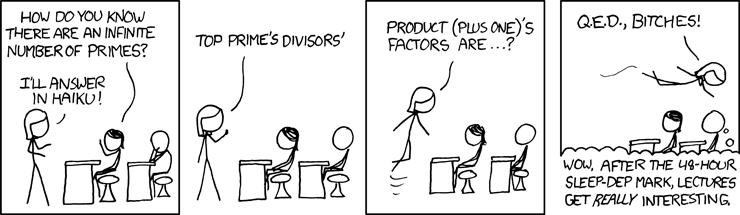
\includegraphics[scale=.5]{comics/622}
\end{center}

\end{multicols}

\section{Mathematik und Gesellschaft}
\begin{multicols}{2}
\label{page:mug}
Die Mathematik. Unendliche Weiten. Dieses sind die Abenteuer einiger
Studenten, die sich auf einer Dreijahresmission in den Tiefen der Räume und
Gruppen befinden, um während ihrer Reise auf der USS Prüfungsordnung neue Sätze
und Formeln zu erforschen. Leider ist der Kontakt zur Mutterzivilisation auf
der Erde längst abgebrochen.

So oder so ähnlich würde die Einleitung einer Fernsehserie zum Studium der
Mathematik wohl lauten. Aber wir sind hier ja nicht im Fernsehen. Und trotzdem
-- oder vielleicht auch gerade deswegen -- klingt es erschreckend realistisch.
Nach allgemeiner Meinung schwebt die Mathematik mehr als jede andere
Wissenschaft im luftleeren Raum. Mathematiker werden im wahren Sinne des Wortes
als weltfremd erachtet. Die Mathematik wird häufig mit Analoga umschrieben:
Mathe sei Kunst, Religion, Sprache, Philosophie, die reinste aller
Wissenschaften. Und doch weiß praktisch niemand was Mathematik wirklich ist.
Vielleicht ist der Kontakt von der Erde ja absichtlich abgebrochen worden?

Wenn man rein berufsorientiert argumentieren will, kann man sagen, dass
Mathematik eine Daseinsberechtigung haben muss, sonst würden Mathematiker nicht
eingestellt werden. Aber welche? Und wie steht es mit der Mathematik und ihren
Anwendungen außerhalb des \emph{echten} Berufslebens? Ist die Mathematik nur
eine Hilfswissenschaft für Physik, Sozial-, Ingenieur- und
Wirtschaftswissenschaften, oder hat sie einen Wert an sich, als \emph{L'art
pour l'art} gewissermaßen?

In der Einheit Mathematik und Gesellschaft am Mittwoch, 12.10. wollen wir uns
mit dieser Problematik auseinander setzen. Was ist Mathematik eigentlich? Was
ist Mathematik nicht? Wie stehen die Mathematik und die Mathematiker in der
Gesellschaft? Tun sie das überhaupt? Wie steht die Gesellschaft zur Mathematik
und zu den Mathematikern? Was kann der Mathematiker von der Gesellschaft
verlangen, was kann, soll und muss er ihr zurückgeben? Und inwiefern ist der
Mathematiker für seine Forschung und deren Wirkungen in die Gesellschaft hinein
verantwortlich?

Selbstverständlich können wir in der kurzen Zeit dieses Thema nicht annähernd
vollständig behandeln -- aber wir werden versuchen, euch Anregungen zu geben.
Wir werden euch mit Fragen konfrontieren, die nicht unbedingt eine Antwort
haben, die man aber trotzdem stellen sollte -- ganz entgegen der landläufigen
Meinung zum Thema Mathematik, die ja auf alle Fragen eindeutige Lösungen kennen
soll (wohlgemerkt: die Mathematik; der Mathematiker kennt sie oft noch nicht).
Außerdem wollen wir aufdecken, wie die Mathematik benutzt oder gar missbraucht
wird, um Objektivität und Sicherheit vorzutäuschen -- dieses Versprechen aber,
wieder entgegen aller Vorurteile, bei weitem nicht immer halten kann.

\begin{center}
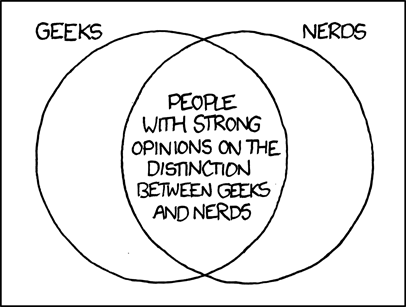
\includegraphics[scale=0.75]{comics/747}
\end{center}

Lange Zeit hat sich die Mathematik weniger um ihre gesellschaftlichen
Verpflichtungen, Berührungspunkte und Zusammenhänge, sondern mehr um sich
selbst gekümmert. Dadurch haben viele Mathematiker die Verwendung ihrer
Arbeiten und den Umgang mit Mathematik in der Gesellschaft und auch in den
anderen Wissenschaften aus den Augen verloren. Unser Wunsch ist es, euch zu
weiterem Nachdenken anzuregen und dass ihr euch mit diesen Fragen
auseinandersetzt, weil es zu verstehen hilft, warum ihr gerade Mathematik
studiert. 

Und weil es hilft, den Kontakt zur Erde vielleicht doch noch aufrecht zu
erhalten.

\end{multicols}

\section{Studentische Interessenvertretung}
\begin{multicols}{2}
\label{page:siv}
Eine Universität ist ein lebendiger Ort! Die Uni verändert sich und ist in
Bewegung: Sie wächst hier und schrumpft vielleicht dort, sie verändert sich von
innen heraus und durch äußere Einflüsse, sie entwickelt Meinungen und
Stellungnahmen, und an all diesen Prozessen sind alle Mitglieder der
Universität beteiligt: Professoren, wissenschaftliche Mitarbeiter, technisches
und Verwaltungspersonal und -- als zahlenmäßig größte Mitgliedergruppe -- die
Studenten! Denn auch wir Studenten sind Teil der Universität und es liegt an
uns, sie zu verändern und zu gestalten! 

Die Möglichkeiten zur Mitgestaltung sind vielfältig: In dutzenden Ausschüssen
der Fakultäten und Fachbereich sitzen studentische Vertreter stimm- und
gleichberechtigt mit den Professoren und anderen Uni-Mitarbeitern zusammen und
machen sich zum Beispiel Gedanken über die künftige strategische Ausrichtung
der Fakultät, die Einführung neuer Studiengänge oder den Lehrveranstaltungsplan
des kommenden Semesters. In all diesen Ausschüssen wird Sacharbeit betrieben,
und zumindest aus dem Fachbereich Mathematik lässt sich berichten, dass die
Studenten dabei durchweg als gleichberechtigte Partner wahr- und ernstgenommen
werden. 

Auch auf Uni-Ebene gibt es Möglichkeiten zur studentischen Mitbestimmung, die
Uni-Gremien kümmern sich jedoch mehr um die \glqq großen\grqq\ Dinge wie z.B.
das Leitbild und Selbstverständnis der Universität. Zudem geht es auf Uni-Ebene
normalerweise deutlich politischer zu als in den Fakultäten und Fachbereichen:
Hochschulpolitische Listen, den großen Parteien nahe stehend, und unabhängige
Listen ringen um die wenigen Plätze im Akademischen Senat und den anderen
Gremien.

Als weitere Säule neben der sachlich geprägten Gremienarbeit in den Fakultäten
gehört zur studentischen Interessensvertretung auch die Selbstverwaltung. Wie
in den meisten Bundesländern bilden auch in Hamburg die Studenten jeder
Hochschule eine sogenannte \emph{Verfasste Studierendenschaft}. Diese verfügt
über einen eigenen Etat und vertritt ihre Interessen selbst. An der Universität
Hamburg geschieht dies über das \emph{Studierendenparlament} (StuPa), welches
jährlich von allen Studierenden gewählt wird. Das StuPa wiederum bestimmt mit
der Mehrheit seiner Vertreter die Mitglieder des \emph{Allgemeinen
Studierendenausschusses} (AStA). Dieser fungiert quasi als Regierung der
Studierenden und hat weitreichende Befugnisse. Daneben ernennt er eine gewisse
Zahl von Referenten für verschiedenen Themenbereiche (Hochschulpolitik,
Soziales, Kultur, \ldots) und bietet Sprechstunden und Beratungen an, zum
Beispiel zu Themen wie BAföG, Studium mit Kind, usw. Eure erste Anlaufstelle
für Probleme dieser Art sollte also der AStA sein. Zu finden ist er auf dem
Campus, gegenüber des WiWi-Bunkers, und unter \url{http://www.asta-uhh.de}.


Während die studentische Interessenvertretung auf dem Campus recht weit
entfernt zu sein scheint, findet ihr auch im Geomatikum eine zuständige
Interessenvertretung: Alle Studenten einer Fachrichtung bilden zusammen eine
Fachschaft. Diese wählt jedes Semester in einer Vollversammlung aus ihrer Mitte
den \emph{Fachschaftsrat} (FSR). Der FSR Mathematik ist also die für euch erste
Anlaufstelle, wenn es um die Vertretung eurer Interessen innerhalb des
Fachbereichs Mathematik geht. Neue Mitglieder sind immer gern gesehen, die
regelmäßigen Sitzungen sind offen für jeden Interessierten und jede Frage oder
Anregung. Näheres zu den Aufgaben und Aktivitäten des FSR findet ihr im Artikel
auf Seite \pageref{page:fsr}.

Es ist ausgesprochen reizvoll, als Student mitgestalten und -bestimmen zu
können. Die Möglichkeiten zur Einflussnahme sind zahlreich und wichtig für die
Situation der Studierenden: Welche Person soll die unbesetzte Professur
übernehmen? Für welche Zwecke sollen die Studiengebühren konkret verwendet
werden? Wie können mehr studentische Arbeitsräume zur Verfügung gestellt
werden? 

Die Mitarbeit in den Gremien schult auch die sogenannten {\it soft
skills}: Selbstbewusstsein, Fähigkeit zu Kommunikation und Diskussion,
Teamwork, usw. Und schließlich knüpft man auf diese Weise sehr enge und
persönliche Kontakte zu den Professoren, was für die Gestaltung des eigenen
Studiums nur von Vorteil sein kann. 

Wer nun neugierig geworden ist und mehr wissen möchte, um vielleicht nach einem
Jahr des Ankommens seine Fühler noch weiter auszustrecken und das Gebilde
Universität besser und von einer ganz anderen Seite kennenzulernen, der schaue
einfach mal unverbindlich beim FSR vorbei.
\end{multicols}

\small
\begin{center}
\begin{tabular}{||p{24mm}||p{73mm}|p{73mm}|p{76mm}||}

\hhline{|t:=:t:=t=t=:t|} & {\bf Ohne Studenten}
    & {\bf Mit studentischer Beteiligung}
    & {\bf Studentische Selbstverwaltung} \\

\hhline{|:=::===:|} {\bf Gesamte Uni}
    & {\bf Hochschulrat}

      \begin{itemize}\itemsep 0pt\parskip 0pt
          \item Wahl des Uni-Präsidenten
          \item Genehmigung von Gebührensatzung, Struktur- und
                Entwicklungsplanung
      \end{itemize}
      {\bf Uni-Präsidium}

      \begin{itemize}\itemsep 0pt\parskip 0pt
          \item Presse- und Öffentlichkeitsarbeit
          \item zentrale Machtbefugniss, Verteilung der Finanzen
      \end{itemize}
    & {\bf Akademischer Senat (AS)}
      
      \begin{itemize}\itemsep 0pt\parskip 0pt
          \item höchstes Gremium, an dem alle Statusgruppen beteiligt sind
          \item stimmt der Wahl des Uni-Präsidenten zu
          \item Präsidium ist dem AS rechenschaftspflichtig
          \item Stellungnahme zu allen Themen in der Universität
      \end{itemize}
    & {\bf Studierendenparlament (StuPa) / AStA}

      \begin{itemize}\itemsep 0pt\parskip 0pt
          \item jährlich von allen Studenten der Universität gewählt
          \item Vertretung politischer, sozialer und kultureller Belange
      \end{itemize} \\
\hhline{||-||-|-|-||} {\bf MIN-Fakultät}
    & {\bf MIN-Dekanat}
      
      \begin{itemize}\itemsep 0pt\parskip 0pt
          \item steht der Fakultät vor, vertritt die Fakultät innerhalb der
                Universität
          \item verfügt über Finanzen der Fakultät, insb. Entscheidung über
                Ausschreibung von Stellen
          \item strategische Ausrichtung der Fakultät
      \end{itemize}

    & {\bf Fakultätsrat (FAR)}
      
      \begin{itemize}\itemsep 0pt\parskip 0pt
          \item berät und kontrolliert das Dekanat, insb. die Verwendung von
                Finanzen
          \item setzt Ausschüsse für Sacharbeit auf Fakultäts- und
                Fachbereichsebene ein
          \item berät über Prüfungsordnungen
      \end{itemize}

    & {\bf MIN-Aktiven-Treffen}

      \begin{itemize}\itemsep 0pt\parskip 0pt
          \item kein formales Gremium, sondern ein gelegentliches Treffen von
                in der Fakultät aktiven Studenten (FSRe)
          \item Informationsaustausch, Absprachen, Planung gemeinsamer
                Initiativen, etc.
      \end{itemize} \\
\hhline{||-||-|-|-||} {\bf Fachbereich Mathematik}
    & {\bf Fachbereichsleitung}

      \begin{itemize}\itemsep 0pt\parskip 0pt
          \item vertritt den Fachbereich in der Fakultät und Universität
          \item verfügt über die Finanzmittel des Fachbereichs
          \item enge Abstimmung mit den Mitgliedern des Fachbereichs
      \end{itemize}

    & {\bf Ausschüsse des FAR}, z.B.

      \begin{itemize}\itemsep 0pt\parskip 0pt
          \item Fachausschuss (FA) Mathematik
          \item Bachelor- und Master-Ausschüsse
          \item Prüfungsausschüsse
          \item Berufungsausschüsse
      \end{itemize}

      {\bf Informelle Kommissionen}, z.B.

      \begin{itemize}\itemsep 0pt\parskip 0pt
          \item Verwendung der Studiengebühren
          \item Entwicklung des Vorkurses
          \item Jahr der Mathematik
      \end{itemize}

    & {\bf Fachschaftsrat (FSR)}

      \begin{itemize}\itemsep 0pt\parskip 0pt
          \item von allen Studenten der Mathematik gewählt
          \item Vertretung der Interessen vor Ort
          \item guter Kontakt zu Professoren und Fachbereichsleitung
          \item Service (Beratung, Prüfungsprotokolle)
          \item Information (Hochschulpolitik, intern)
          \item Vernetzung im Fachbereich
          \item Freizeit (Kartenspielen, Weihnachtsfeier, Parties, etc.)
      \end{itemize} \\
\hhline{|b:=:b:===:b|}
\end{tabular}
\end{center}
\begin{multicols}{2}

\normalsize

Dieses Schaubild soll euch einen Überblick über die verschiedenen, relevanten
Gremien auf Universitäts-, Fakultäts- und Fachbereichsebene geben. Näheres zu
den Gremien und ihren Zuständigkeiten erfahrt ihr in der Einheit Studentische
Interessenvertretung. Sollten noch Fragen offenbleiben, kann euch der FSR
weiterhelfen, der sich über Besuch immer sehr freut. Die regelmäßigen Sitzungen
sind öffentlich.

\end{multicols}

\section{Vorstellung}
\begin{multicols}{2}[\subsection{Studienbüro Mathematik}]

Das Studienbüro Mathematik ist die zentrale Anlaufstelle für alle Fragen rund
um das Studium am Fachbereich Mathematik. Wir vereinen die bisherige
Prüfungsstelle, die Studienfachberatung sowie die Koordination der Studiengänge
und weitere Aufgaben unter einem Dach und arbeiten eng mit dem Beauftragen für
Studium und Lehre und unseren Prüfungsausschüssen zusammen. 

Für Sie als Studierende wird das Studienbüro besonders in Fragen der Prüfungs-
und Veranstaltungsverwaltung eine wichtige Anlaufstelle sein. Sie sind bei uns
richtig für

\begin{itemize}\itemsep 0pt
    \item Fragen zur Prüfungsordnung 
    \item Fragen oder Schwierigkeiten bei der Anmeldung von Modulen,
          Veranstaltungen und Prüfungen
    \item Fragen zum Leistungskonto (elektronische Prüfungsakte)
    \item Bescheinigungen abholen und einreichen
    \item Krankmeldungen
    \item Anerkennungen
    \item Zeugnisse
    \item u.v.m.
\end{itemize}

Abhängig von Ihrem Anliegen empfehlen wir die folgenden Kontaktwege zu nutzen:

\begin{itemize}\itemsep 0pt
    \item Sämtlich STiNE-Angelegenheiten (Anmeldungen,
          Web-Leistungskonto): das Supportformular in STiNE
    \item Allgemeine Anfragen (Bsp: Terminanfragen für Beratungen, Erstellung
          von Bescheinigungen): studienbuero@math.uni-hamburg.de
    \item Beratungen, Abgabe oder Abholung von Unterlagen: persönlich, während
          der Öffnungszeiten oder nach Terminvereinbarung. 
\end{itemize}

\columnbreak

Auf unseren Webseiten finden Sie wichtige Informationen, Kontaktdaten,
Formulare und aktuelle Hinweise:
\url{http://www.math.uni-hamburg.de/studienbuero/}

Wir wünschen Ihnen viel Freude und Erfolg für Ihr Studium!

Ihr Studienbüro Mathematik-Team

\begin{center}
\vfill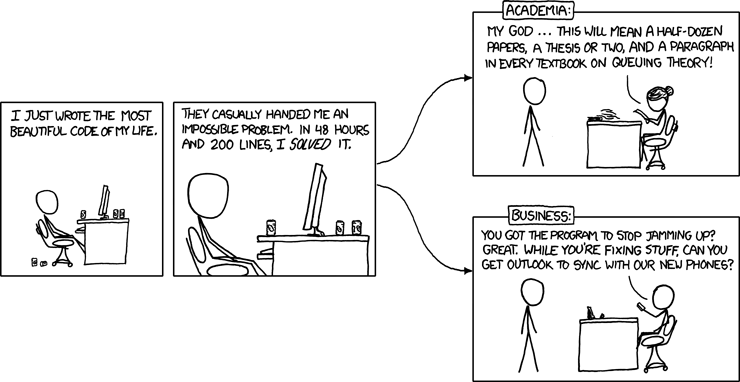
\includegraphics[scale=.5]{comics/664}
\end{center}

\end{multicols}

\clearpage

\begin{multicols}{2}
\subsection{FSR Mathematik} \label{page:fsr}

Unsere Aufgabe ist es, die Interessen der Fachschaft -- das seid ihr und alle
anderen Mathematik-Studenten am Fachbereich Mathematik der Universität Hamburg
-- zu vertreten. Wir werden zu Beginn jedes Semesters auf einer Vollversammlung
aller Mathematik-Studenten gewählt und kümmern uns dann um alles, was so
anliegt.

Konkret bedeutet das: Wir beobachten, was hier am Fachbereich, in der Fakultät,
an der Uni und sonst wo vor sich geht und mischen uns wenn nötig ein und
informieren euch über alles Wichtige durch unseren E-Mail-Newsletter (hierfür
nutzen wir die Mailinglisten des Fachbereichs -- also ganz schnell eintragen!)
und Aushänge in unserem Infokasten (zwischen den Fahrstühlen und der
Pförtnerloge neben dem schwarzen Brett) oder der Pinnwand neben dem T30. Bei
wichtigen Anlässen berufen wir auch während des Semesters Vollversammlungen
(VV) ein, auf denen wir mit euch das weitere Vorgehen besprechen. Dies geschah
in der Vergangenheit vor allem zu Streiks oder Aktionen gegen Studiengebühren.

Darüber hinaus sind wir eure Ansprechpartner für Probleme mit eurem Studium und
für Fragen aller Art. Wir wissen zwar auch nicht auf alles eine Antwort, aber
haben dann meistens eine Idee, wer euch weiterhelfen kann.

Wir unterhalten auch eine Sammlung von Prüfungsprotokollen, die euch zur
Vorbereitung auf eure eigenen Prüfungen sicher hilfreich sein kann. Diese lebt
von der Mithilfe aller, das heißt wer eine Prüfung absolviert hat, sollte im
Anschluss ein simples Gedächtnisprotokoll verfassen und über die Datenbank auch
anderen zur Verfügung stellen. So bleibt die Sammlung stets möglichst aktuell,
und alle haben einen Nutzen davon. Gerade über die Prüfungen in den
Bachelorstudiengängen gibt es natürlich noch kaum Protokolle, also wäre es sehr
hilfreich Kopien der Klausuren zu bekommen.

Ansonsten veranstalten wir als FSR auch noch diverse Aktionen für euch, wie zum
Beispiel jeweils ein Skat- und Pokerturnier, öfters mal
Überraschungswunschfilmabende, jährliche Weihnachtsfeiern, seltener
Spieleabende sowie ab und zu Partys oder ein Sommergrillen und was uns gerade
sonst noch so einfällt -- oder von euch gewünscht wird. Falls ihr eine Idee
oder eine Wunsch habt, was veranstaltet werden könnte, meldet Euch einfach bei
uns!

Im Semester gibt es meistens feste Sprechzeiten, während der ihr auf jeden Fall
einen von uns im T30 antreffen solltet. Ansonsten erreicht ihr uns per Mail an
\href{mailto:fsr@math.uni-hamburg.de}{fsr@math.uni-hamburg.de}.

Der Fachschaftraum T30 ist übrigens ein studentischer Aufenthaltsraum, der
allen Studenten offen steht. Hier findet ihr neben der Datenbank mit
Prüfungsprotokollen eine kleine Präsenzbibliothek, welche vor allem die gängige
Anfängerliteratur zum schnellen Nachschlagen oder einfach mal so Stöbern
bereithält. Ansonsten liegen dort auch immer mal wieder aktuelle
Informationsmaterialien, die für jeden interessant sein können.

Aber auch alles, was man braucht, um sich mal eine kleine Lernpause zu gönnen,
findet ihr im T30. Es gibt Getränke zum Selbstkostenpreis, Geschirr für eure
selbst mitgebrachte Mahlzeit, falls die Mensa schon zu hat (dieses ist nach
Benutzung wieder zu reinigen) und meist auch einige motivierte Mitspieler für
die eine oder andere Doppelkopf-, Poker- oder Skatrunde oder einfach offene
Ohren, um mal ein wenig Lernfrust abzulassen oder sich einen Lösungstipp zu
holen.

Wer Lust hat, mehr über uns zu erfahren und vielleicht sogar bei uns
mitzuarbeiten, ist herzlich zu einem Besuch im T30 oder auf unserer Homepage
\url{http://www.math.uni-hamburg.de/fsr} eingeladen.

In den nächsten Wochen findet die Wahl des neuen FSR statt. Dabei wird über das
Programm für das Semester diskutiert, also kommt zur Vollversammlung und bringt
eure Wünsche und Vorstellungen ein. Achtet dazu auf Ankündigungen am Infobrett
und auf der Tafel im Foyer.

\hfill euer FSR Mathematik


% Informationen zu den Öffnungszeiten.
% http://www.math.uni-hamburg.de/home/jampert/formulare/index_o.html#oeffnung-cip
\subsection{CIP-Pool}

Am Fachbereich Mathematik stehen euch auch Arbeitsplätze zur Verfügung, die mit
einem Computer ausgestattet sind. Diese findet ihr in den sogenannten
CIP-Pools, die sich in der ersten Etage des Geomatikums befinden. Neben einer
großen Anzahl von Computern mit Betriebssystem Windows gibt es auch einige
Computer auf denen UNIX als Betriebssystem installiert ist. Sämtliche Computer
sind mit mathematischer Software, einem Zugang zum Internet und einem
persönlichen Speicherplatz ausgestattet.

\subsubsection{Zugang zu den Computern}

Die Räume des CIP-Pools sind sowohl in der Vorlesungszeit als auch in den
Semesterferien regelhaft von 10:00 bis 16:00 Uhr geöffnet. Die Öffnungszeiten
werden nicht all zu streng gesehen, sodass es einerseits häufig kein Problem
ist, länger zu arbeiten, andererseits die Verfügbarkeit nicht unbedingt immer
um 10:00 Uhr beginnt. Im zweiten Fall lohnt es sich häufig im selben Stockwerk
beim Verwaltungspersonal nachzufragen, ob die Räume aufgeschlossen werden
können.

Um einen der Computer benutzen zu können, müsst ihr euch mit eurer persönlichen
Kennung anmelden. Diese wird euch auf dem Postweg mitgeteilt. Falls ihr eure
Zugangsdaten nicht erhalten haben solltet, so könnt ihr diese beim
Rechenzentrum, in der Schlüterstraße 70, oder bei den Aufsichten des CIP-Pools
beantragen. Die Bearbeitung nimmt allerdings mindestens einen Tag in Anspruch.
Eure Zugangsdaten bestehen aus einer persönlichen Kennung sowie einem Passwort.
Beim Anmelden an einem Computer müsst ihr zudem noch eine Nutzergruppe angeben,
die für Studenten des Fachs Mathematik oder Wirtschaftsmathematik \glqq
Studi\grqq, für Studenten des Lehramts mit Fach Mathematik \glqq Erzwiss\grqq\
lautet. Die Gruppe \glqq Mathe\grqq\ ist Mitarbeitern an der Fakultät
vorbehalten.

Nach einer ersten erfolgreichen Anmeldung empfiehlt es sich, das eigene
Passwort zu ändern. Das könnt ihr unter \url{http://www.rrz.uni-hamnburg.de}
$\rightarrow$ Benutzung des RRZ $\rightarrow$ Passwort tun. Achtet darauf, ein
ausreichend sicheres Passwort zu wählen!

%\begin{center}
%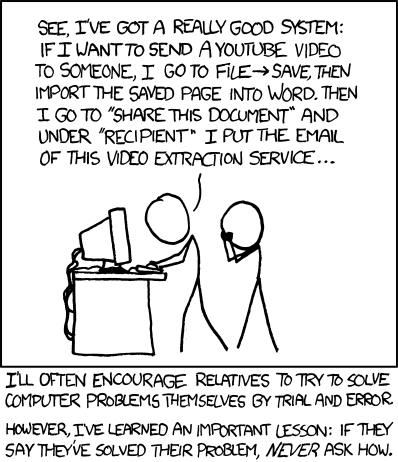
\includegraphics[scale=.5]{comics/763}
%\end{center}

\begin{center}
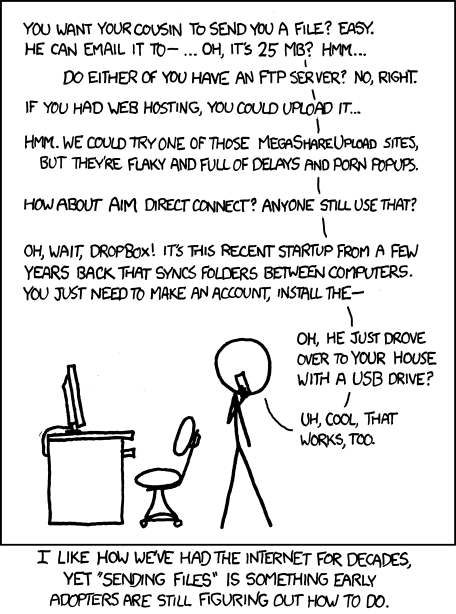
\includegraphics[scale=.65]{comics/949}
\end{center}

\subsubsection{Speichern und Drucken}

Eines der leidigsten Themen an dem eigenen Laptop ist das Drucken in fremder
Umgebung. Dafür eignen sich die Computer in den CIP-Pools außerordentlich gut,
denn die Computer sind hier bereits konfiguriert und außerdem stellt der
Fachbereich Mathematik jedem Studenten ein monatliches Druckkontingent zur
Verfügung. Dieses kann an den Computern überprüft werden und durch einen
Druckauftrag an den Drucker l142, welcher sich -- wer hätte es geahnt -- im
Raum 142 befindet, in nahezu beliebig bedrucktes Papier verwandelt werden. Es
empfiehlt sich, im CIP-Pool nicht am letztmöglichen Tag und schon gar nicht im
letztmöglichen Moment etwas drucken zu wollen. Zu häufig hat man dafür mit den
üblichen Problemen -- kein Papier mehr, Düsen verstopft, Toner alle, keine
Netzwerkverbindung, Sanduhr, Sanduhr, Sanduhr, \dots -- zu kämpfen. In einem
solchen Fall wendet man sich am besten an die Aufsichten des CIP-Pools, die
sich entweder in den Computer-Räumen oder im Raum nebenan aufhalten.

Eines der leidigsten Themen an einem fremden Computer ist der Dateitransfer.
Glücklicherweise sind die Computer mit USB-Schnittstellen sowie einem
Netzlaufwerk ausgestattet, sodass man nicht voller Verlegenheit eine E-Mail an
sich selbst adressieren muss. Zudem besitzt jeder Student einen persönlichen
Speicherplatz von 20 MB, der von jedem Computer aus erreichbar ist und sobald
man sich anmeldet als ein Laufwerk (Windows) oder Mount-Point (UNIX)
eingebunden wird. Ihr solltet darauf achten, keine persönlichen oder wichtigen
Daten auf dem Computer außerhalb eures Netzlaufwerkes zu speichern. Zum einen
kann jemand, der den Computer nach euch benutzt, gegebenenfalls darauf
zugreifen. Zum anderen werden einige Speicherbereiche automatisch, andere
manuell durch die Administratoren gelöscht.

\subsubsection{E-Mail}

Jeder Student der Universität Hamburg erhält eine persönliche E-Mail-Adresse
nach dem folgenden Muster. Was passiert, falls zwei eingeschriebene Studenten
dieselben Namen aufweisen, haben wir leider noch nicht in Erfahrung bringen
können.

\url{vorname.nachname@studium.uni-hamburg.de}

Auf das Postfach dieser Adresse könnt ihr im Portal des Rechenzentrums
zugreifen. Dazu besucht ihr die Homepage des Rechenzentrums unter
\url{http://www.rrz.uni-hamburg.de} und wählt dort den Verweise auf Surfmail.
In dem folgenden Formular könnt ihr euch mit derselben Kennung anmelden, mit
der ihr die Computer in dem CIP-Pool nutzen könnt.

\end{multicols}

\section{Tipps}
\begin{multicols}{2}
\subsection{Was die Uni so alles zu bieten hat}

\subsubsection{Wo bitte geht's zum Rechnen?}

Zum Lernen und Arbeiten stehen im Geomatikum folgende studentische Arbeitsräume
zur Verfügung: im Erdgeschoss E24, im Techniker-Geschoss die Räume T27, T33,
T35 und T37 (und natürlich der FSR (T30), wobei dieser Raum in erster Linie ein
Aufenthaltsraum ist und es daher dort normalerweise etwas lauter ist), im 2.
Stock die Räume 242 und 244 und im 4. Stock der Raum 427. Außerdem dürft ihr
natürlich in allen Übungsräumen arbeiten, solange dort keine Veranstaltungen
sind. Desweiteren gibt es noch einen Gruppenraum in der Bibliothek, in der man
natürlich auch an den Lesetischen still arbeiten kann. Da das Geomatikum am
Samstag ab 13 Uhr und am Sonntag durchgehend geschlossen ist, bietet sich für
diese Zeit die Staatsbibliothek (Stabi), geöffnet Montag bis Freitag von 9-21,
Samstag von 10-18 und Sonntag von 12-18 Uhr, an. Dort gibt es Lesesäle zur
ruhigen Arbeit und Bereiche, in denen sich Gruppen unterhalten dürfen.

\subsubsection{Ich hab' Hunger!}

Schon bald werdet ihr unsere heimische Geomatikum-Mensa das erste Mal leid
sein. Dann empfiehlt sich ein Besuch auf dem Campus in einer der drei großen
Mensen im Philosophenturm, WiWi-Bunker oder der alten Hauptmensa hinter dem
Audimax. In den ersten beiden locken große Salatbuffets, eine Pastabar und eine
Wok-Station. Sehr gut ist auch die TU-Mensa in Harburg. Aber nach einiger Zeit
werdet ihr bestimmt des dauernden Laufens überdrüssig werden und reumütig ins
Geomatikum zurückkehren\ldots

\subsubsection{Schwitzen leicht gemacht}

Als Ausgleich zu der vielen kopflastigen Arbeit des Studiums eignet sich ein
Sport sehr. Über das Hochschulsportprogamm
(\url{http://www.hochschulsport-hamburg.de}), welches allen Hamburger Studenten
und -- gegen Aufpreis -- allen Mitarbeitern der Hochschulen und auch Externen
offensteht, erhaltet ihr ein umfassendes Angebot: von Rudern und Segeln auf der
Alster über alle gängigen Ballsportarten bis zu Kampfsport, Yoga, Bogenschießen
und die Teilnahme im Hochschulsport-Fitnessstudio -- hier findet jeder seine
Sportart.  Die Preise sind günstiger als in Vereinen.

\subsubsection{Qu\'{e} hablas?}

Wer mit seinem Studium noch nicht genug ausgelastet ist und seine
Fremdsprachenkenntnisse auffrischen oder ausbauen möchte, hat hierzu zwei
Möglichkeiten. Das Fachsprachenzentrum der Uni bietet Kurse auf hohem Niveau zu
verschiedenen Themengebieten an, in denen Fach- und Vokabelwissen kombiniert
werden. Zur Teilnahme muss man an einem Einstufungstest zu Beginn des Semesters
teilnehmen -- auf die neonfarbenen Plakate achten! Wer das erforderliche Niveau
nicht nachweisen kann, kann dieses in den Fremdsprachenkursen der
Volkshochschule in Kooperation mit der Universität erwerben. Neuerdings sind
diese Kurse kostenlos, eine frühzeitige Anmeldung ist daher zu empfehlen.
Informationen zu beiden Arten von Kursen findet ihr unter
\url{http://www.uni-hamburg.de/fremdsprachen.html}.

\subsubsection{Hilfe!}

Viele Studenten geraten im Laufe ihres Studiums mindestens einmal in eine Krise
und fragen sich dann: Studiere ich das Richtige? Bin ich überhaupt für die Uni
geeignet? Warum komme ich nicht mit? Manchmal kommen dann noch persönliche
Krisen und Probleme hinzu, die das Studium erschweren oder sogar unmöglich
machen. Solltet ihr irgendwann im Verlauf eures Studiums mit Problemen dieser
Art zu kämpfen haben, und helfen euch auch Gespräche mit Freunden und
Kommilitonen nicht weiter, dann legen wir euch das Zentrum für Studienberatung
und Psychologische Beratung der Universität wärmstens ans Herz (über
\url{http://www.uni-hamburg.de} $\rightarrow$ Studierende $\rightarrow$ Zentrum
für\ldots).  Neben einer kostenlosen, persönlichen und umfassenden Betreuung
und Beratung bietet das Zentrum auch Kurse und Workshops an, beispielsweise zur
Bekämpfung von Prüfungsangst, dem Sprechen vor einer Gruppe oder selbständigem
Arbeiten.

\subsubsection{Soft skills -- starke Fähigkeiten}

Das Zentrum für Studienberatung und Psychologische Beratung bietet auch andere
Kurse an, die auf eine Stärkung der sogenannten \emph{soft skills} abzielen.
Das sind unter anderem freies Sprechen, Lern- und Arbeitstechniken,
Stressbewältigung, Zeit- und Selbstmanagement. Auch das Career Center der
Universität ({\tt www.uni-hamburg.de} $\rightarrow$ Studierende $\rightarrow$
Career Center) bietet Kurse dieser Art, Vorträge und andere Veranstaltungen an,
die der Berufsorientierung dienen. In der Regel sind diese Veranstaltungen
kostenlos, eine Anmeldung ist für die Kurse jedoch erforderlich.

\subsubsection{Das liebe Geld}

Oft leiden Studenten unter chronischem Geldmangel. Die Universität und der
Fachbereich bieten durch zahlreichen Tutoren- und Hilfskraft-Tätigkeiten die
Möglichkeiten für kleine Zuverdienste an. So arbeiten Studenten etwa als
Aufsicht in der Bibliothek oder in den Computerräumen, und für die etwas
fortgeschrittenen Semester gibt es natürlich viele Jobs als Korrektor von
Übungsaufgaben, Übungshelfer oder sympathischer und munterer Tutor der
Orientierungseinheit. Auch an anderen Einrichtungen und Instituten der Uni gibt
es Jobs für Studenten. Haltet einfach Augen und Ohren offen und hört euch aktiv
um, indem ihr Professoren und Studenten höherer Semester ansprecht.

\subsection{Was Hamburg so alles zu bieten hat \dots}

Im folgenden haben wir einige praxiserprobte Tipps zusammengestellt, mit denen
ihr eure Freizeit in dieser wunderbaren Stadt gestalten oder auch nur eure
Freistunden füllen könnt.

\subsubsection{Caf\'es}

Wem die Cafeteria im Geomatikum zu ungemütlich ist, findet auf dem Weg zum
Campus mehrere Caf\'e-Alternativen an der sogenannten \emph{Grindelmeile}.  Von
der Stabi bis zu den Grindelhochhäusern drängen sie sich dicht an dicht: je
nach Ausrichtung gibt es dann dazu z.B. Fußball live (Campus Caf\'e), Milchreis
in verschiedenen Varianten (Caf\'e R-Eis), viel Bio (Caf\'e Aramon), einen
Friseur (Gute Köpfe), preiswertes Frühstück (Caf\'e Backwahn) oder Lesungen und
Bücher-Stöber-Kisten (Caf\'e Mathilde (Ecke Beim Schlump/Bogenstraße) und Bar
Mathilde (beim Abaton-Kino), \url{http://www.mathilde-hh.de}).

\begin{advice}{Alex}
Das Hadley's ist ganz nah am Geomatikum in einem ehemaligen Krankenhaus
untergebracht (Beim Schlump 84a). Im Sommer kann man im wunderschönen und
ruhigen Innenhof sitzen und Trinkschokolade in fünf Geschmacksrichtungen
genießen. Im Inneren locken gemütliche Sofas und Sessel.
\end{advice}

Wer's gerne hip mag, trinkt sein Koffein-Heißgetränk in der Schanze auf der
sogenannten \emph{Gal\~{a}o-Meile} (Schulterblatt und angrenzende Straßen).
Gegenüber vom Zentrum der linken Szene, der Roten Flora, kann man hier sehen
und gesehen werden und nach dem Milchkaffee noch trendig shoppen.

Bekannt für gutes Eis und ausgefallene Sorten sind die Filialen von Eiszeit
(Müggenkampstraße~45, Mühlenkamp~46 und Falkenried~47). Am nähesten beim
Geomatikum ist das Eiscaf\'e La Veneziana an der Grindelallee.

\begin{advice}{Svenja}
Bei Eisliebe in Altona (Bei der Reitbahn 2) gibt's das beste Eis, ein kleiner
Laden mit sehr vielen Sorten. Und wenn man schon mal in Altona ist, gleich noch
im Bonscheladen (Friedensallee 12) vorbeischauen, hier werden Bonbons selbst
gemacht.
\end{advice}

\subsubsection{Fast Food}

\begin{advice}{Adam}
Die besten Döner gibt's bei Dubara: Jarrestraße~57, Wandsbeker Marktstraße~47,
Schlossmühlendamm (Harburg).
\end{advice}

Die nächsten McDonald's-Filialen sind am Dammtor-Bahnhof und an der U-Bahn
Hoheluft. An der Grindelallee gibt es die Sandwiches von Subways. Zahlreiche
Döner-Läden liegen ebenfalls auf der Strecke zwischen Campus und Geomatikum.
Außerdem sorgen viele asiatische Imbisse rund um die Kreuzung der Grindelallee
und Rentzelstraße für Abwechslung. Als einziger Pizzaservice liefert Joey's ins
Geomatikum. Eine Preisliste liegt im FSR (Raum T30).

\begin{advice}{Alex}
Der Curry-Grindel (Renzelstraße~4) ist ein Muss für jeden, der einmal in
Hamburg ist. Hier gibt es eine große Auswahl an hervorragenden Curry-Würsten.
Dazu den berühmten Gurkensalat und das alkoholfreie Ingwer-Bier. Mit Hamburger
Hafen-Flair werden die Gerichte an den Mann gebracht. Das entschädigt auch die
moderaten Preise.
\end{advice}

\subsubsection{Essen und Trinken}

Die oben genannten Caf\'es bieten meist auch Snacks und Salate. Wer etwas mehr
braucht, wird vielleicht in der Geomatikum-Stammkneipe Geo 53 (gute Pizzen,
Mittagstisch, auch zum Mitnehmen; Beim Schlump 53), im Roxie (Burger,
Sandwiches und Co, mit Biergarten; Rentzelstraße~6) oder im Down Under
(berühmt-berüchtigt: Chicken Wings all you can eat; Ecke
Grindelallee/Bundesstraße) fündig.

\begin{advice}{Kathrin}
Gute und bezahlbare Burger in netter Atmosphäre gibt's bei Doris Diner
(Grindelhof 43). Frühstücken kann man in aller Ruhe im Mangold Lokal (Ölmühle
30, U Feldstraße).
\end{advice}

Das Bistro des Abaton-Kinos (Allende-Platz) hat tolle Gerichte für faire
Preise. Im Sommer kann man man draußen sitzen. Wer nach dem Besuch des Holi-Kinos (Ecke
Schlankreye/Grindelberg) noch einen schnellen Happen braucht, sollte im kleinen
Senza Nome (Lehmweg 6) die \emph{Pizza Speck} probieren. Wenn's etwas mehr sein darf,
hat der große Nachbar Block House (Ecke Hoheluftchaussee/Lehmweg)
hervorragendes Fleisch. Sein etwas lässigerer Ableger ist Jim Block
(Fuhlsbüttler Str.~165, Kirchenallee 37), wo aus dem gleichen guten Fleisch
tolle Burger gemacht werden.

In der Schanze findet der spät aufgestandene Student viele Orte für ein spätes
Frühstück, z.B. in Omas Apotheke oder dem Frank und Frei (Ecke
Schanzenstraße/Susannenstraße). Ebenfalls in der Schanze gibt es gleich zwei
Ableger der Bok-Restaurants (Schulterblatt 3, Schanzenstraße~27), die für etwas
gehobenere Preise asiatisches Essen aus mehreren Ländern anbieten, von Sushi
bis Ente süß-sauer.

\begin{advice}{Clara}
Am Allende-Platz gibt es einen Imbiss mit gefüllten Ofenkartoffeln (Kumpir) zum
studentengerechten Preis für 2 bis 4 Euro, wobei für die Füllungen nicht nur
Sour Cream, sondern eine große Zahl von Zutaten zur Verfügung steht: Spinat,
Pepperoni, Mais, Champignons, Thunfisch, Schafskäse, verschiedene Soßen und
vieles mehr. Sattwerden garantiert!
\end{advice}

Ein paar Ecken weiter (Ecke Wohlwillstraße/Brigittenstraße) gibt es in der
Trattoria da Rocco alles, was das Italiener-Herz begehrt, inklusive einer
lautstarken \glqq Buena sera!\grqq-Begrüßung. Ebenfalls italienisch, aber in
modernem Ambiente und zum Zugucken wird im Vapiano (Ecke
Rothenbaumchaussee/Turmweg) gekocht. Die günstigen Preise von 5 bis 8 Euro
locken mittags Büroleute und abends Harvestehudes Schickeria an. Das Altamira
in Ottensen (Thomasstraße) bietet eine große Auswahl an leckeren Tapas, hier
ist für jeden Geschmack etwas dabei. Im sogenannten \emph{Portugiesen-Viertel}
(die Straßen zwischen Michel und Elbufer) verbringt auch Otto Waalkes gerne den
Abend in einem der (meist Fisch-)Restaurants. Das Restaurant Mongolei
(Wandsbeker Zollstraße~155) hat für 12,80 Euro täglich ein Büfett mit
zahlreichen asiatischen Gerichten zu bieten. Das Fleisch wählt man selbst aus
und bekommt es vor seinen Augen nach Wunsch gebraten.

Eine Cocktailbar mit großer Auswahl findet man im Gebäude der U-Bahn Mundsburg,
das Ambiente ist aber etwas kühl und die Preise für 6 Euro normal bis hoch. Auch
im Down Under (s.o.) gibt es Cocktails (montags für 5,10 Euro). In der Turmbar
des Hotel Hafen Hamburg (Landungsbrücken) ist auf die Cocktailpreise die
fantastische Aussicht draufgeschlagen.

\subsubsection{Weggehen}

Wenn im Frühjahr die ersten wärmeren Sonnenstrahlen locken, kurbelt der
Hamburger nicht nur sofort sein Cabrio-Verdeck herunter, sondern erfreut sich
seit einigen Jahren vor allem an den Beach Clubs, die an mehreren Standorten in
Hamburg, vor allem entlang des Elbufers hinter dem Fischmarkt, den Sommer über
aufmachen. In allen wird feiner Sand in großen Mengen ausgekippt, Liegestühle,
Hängematten, teilweise Sofas und Liegewiesen locken zum Verweilen, während man
den Containerschiffen auf der Elbe zuschaut. Bei entsprechenden Preisen gibt es
Cocktails und andere Getränke, manchmal auch Snacks oder Gegrilltes. Schaut
einfach im nächsten Frühling in die Zeitungen, wo es dieses Mal Clubs gibt.

\begin{advice}{Dennis}
Eine grandiose Cocktailbar ist das Cairos (Hoheluftchaussee~117). Der beste
Cocktail: der \emph{Pangalaktische Donnergurgler}. Danach zum Billardspielen
oder zum Kickern an Hamburgs längsten Kickertisch ins Queue (Fuhlsbüttler
Straße~184).
\end{advice}

Wer's etwas gemütlicher mag, findet in der Schanze rund um das Schulterblatt
dicht an dicht Locations, in denen man den Abend verbringen oder auch nur ein
wenig vorglühen kann. Am frühen Abend und bei entsprechendem Wetter werden auch
Bierbänke nach draußen und in die Hinterhöfe gestellt. Zu späterer Stunde
strandet man dann gemütlich in der Sofabar (Ecke Schanzenstraße/Beckstraße).

Unbestrittenes Herz des Hamburger Nachtlebens ist der Kiez. Das sind die
berühmt-berüchtigte \emph{Reeperbahn} und ihre Nebenstraßen, vor allem die
Große Freiheit, mitten in St.~Pauli gelegen. Für ausgedehntes Kneipen-Hopping
als Einstieg für einen gelungenen Party-Abend empfehlen sich die zahlreichen
kleinen Läden in der Straße Hamburger Berg, darunter Roschinsky's, Rosie's Bar,
der Blaue Peter und die Barbarabar. Auch rund um den Hans-Albers-Platz gibt es
diverse Kneipen und Bars.

\begin{advice}{Arne}
In der Talstraße~22 gibt es die Bar 3-Zimmer-Wohnung. Die Theke befindet sich
in der Küche, gemütlich sitzen lässt es sich im Wohnzimmer. Im Schlafzimmer
wird eine Partie Playstation gespielt. Eine gemütlich eingerichtete Bar, mit
Büchern zum Stöbern und Kickertisch, zum einfach nur wohlfühlen -- und das
mitten auf dem Kiez!
\end{advice}

\subsubsection{Clubs}

Der Club mit der größten Tradition ist zweifelsohne die Große Freiheit (Große
Freiheit~36). Hier sind schon alle möglichen Größen des Musikgewerbes
aufgetreten, auch heute gibt es hier noch oft Konzerte. An den anderen Abenden
bietet die Freiheit meist eine bunte Mischung auf dem Main-Floor, im Keller
Alternative und härteren Rock und in der Galerie Latino-Musik. Gleich nebenan
liegt das Grünspan (Große~Freiheit~58), \glqq Hamburgs Rockcenter No.~1\grqq
laut Eigenwerbung. Auch hier gibt es oft Konzerte.

Das Molotow (Spielbudenplatz~5) ist seit Jahren eine feste Größe auf dem Kiez.
Verschiedene DJs, Clubpartys und Events sorgen für Abwechslung, die Preise sind
vertretbar. Zum Aufwärmen eignet sich die Meanie Bar im selben Gebäude,
Eigenbeschreibung: \glqq Das Spektrum reicht musikalisch von französischen
Chansons und Beatperlen über schräge Experimental-Elektronik,
Sixties-Psychedelia bis hin zu russischer Folklore.\grqq

Der Golden Pudel Club direkt am Fischmarkt (Nr.~27) glänzt durch entspannte
Atmosphäre, ein interessant gemischtes Publikum, darunter auch immer wieder
Szenegrößen, und stimmige Musik von Elektro bis Hip-Hop, je nach DJ. An den
Wochenenden ist es oft brechend voll, im Sommer verlagert sich die chillende
Menge auf die angrenzenden Treppen mit Blick auf den Hafen.

Und wenn man schon einmal da ist, kann man auch gleich die Nacht durchmachen,
denn der unbestritten typischste Ausklang einer Party-Nacht führt einen am
Sonntagmorgen auf den \emph{Fischmarkt} (Große Elbstraße, nicht weit vom Kiez),
auf dem ab 4 Uhr echte Hamburger Originale wie \emph{Aale-Dieter} oder
\emph{Bananen-Benno} ihre Waren an den Mann bringen. Ein frisches Fischbrötchen
ist hier ein Muss. Um 7 Uhr, spätestens 8 Uhr ist der Zauber dann auch schon
wieder vorbei.

\subsubsection{Sonne tanken}

Gemütlich in der Sonne chillen kann an vielen Stellen in Hamburg, die Stadt
gilt nicht umsonst als eine der grünsten Städte Deutschlands. Besonders schön
hat man es auf den Alsterwiesen entlang des Harvestehuder Wegs mit Blick auf
die am Wochenende zahlreichen Jogger, Segler und Ruderer. Hier wird auch gerne
mal gegrillt. Auch am Gegenufer (Ostseite) gibt es ein paar grüne
Liegeflecken.

Der Elbstrand ist schon lange kein Geheimtipp mehr. Hier fühlt man sich fast
wie im Urlaub, nur dass eine beeindruckende Szenerie vorbeiziehender
Containerriesen hinzukommt. Zu Ostern werden an vielen Stellen große Lagerfeuer
entzündet und sorgen für eine schöne Stimmung. Grillen wird hier meist
toleriert, wenn man keinen Müll zurücklässt und die heiße Asche sicher
entsorgt. Leider ist der Övelgönner Strand etwas schwer zu erreichen, am besten
aber noch mit dem Bus 112 (von Bahnhof Altona) oder der Hafenfähre 62 (von
Landungsbrücken) bis Neumühlen. Ansonsten gibt es einige nur zu Fuß passierbare
Zugänge von der Elbchaussee aus (z.B. Himmelsleiter und Schulberg). Oder man
nähert sich vom anderen Ende, von Teufelsbrück aus.

Unter der Woche angenehm leer, am Wochenende brechend voll ist der Stadtpark
(zu erreichen über U Borgweg, U Saarlandstraße oder S Alte Wöhr, der Bus 179
hält vor dem Planetarium). Hier wird Fußball gespielt, jongliert, gegrillt oder
nur auf der Wiese entspannt, im Stadtparksee gibt es ein Freibad. Wer die
Eintrittskarten für die sommerlichen Open Air Konzerte auf der Freilichtbühne
(S Alte Wöhr) sparen möchte, kann auch von einer der angrenzenden Wiesen aus in
den vollen akustischen Genuss kommen.

\subsubsection{Anschauen}

Hamburg beherbergt zahlreiche Museen zu den verschiedensten Themen: Kunsthalle,
Völkerkundemuseum, Museum der Arbeit, Museum für Kunst und Gewerbe, Zoll- und
Gewürzmuseum und andere. Eine Anregung findet man unter
\url{http://www.freizeitziele.hamburg.de}.

\begin{advice}{Monika}
Einmal im Jahr findet die \emph{Lange Nacht der Museen} statt. Einmal das
Ticket gezahlt, kann man die ganze Nacht alle Museen Hamburgs besuchen. Eine
ideale Möglichkeit, um überall einmal reinzuschnuppern, auch wenn es ziemlich
voll ist. Was einem gefallen hat, kann man ja später nochmal in Ruhe besuchen.
\end{advice}

Das Miniatur Wunderland (\url{http://www.miniatur-wunderland.de}) in der
Speicherstadt ist die größte Modelleisenbahn der Welt, eine unglaubliche
Vielfalt in Größe H0 bietet sich den Besuchern. Hier werden gestandene
Familienväter wieder zu Kindern und können sich nicht losreißen von den
Szenerien, die u.a. Hamburg, die Alpen, Amerika und Skandinavien darstellen und
mit Liebe zum Detail begeistern. Die Anlage wird ständig ausgebaut. Eine
Kartenreservierung empfiehlt sich, um Wartezeiten zu vermeiden.

Das Planetarium im Stadtpark (\url{http://www.planetarium-hamburg.de}) besitzt
eine der modernsten Projektionsanlagen weltweit und bietet ständig wechselnde
Veranstaltungen an, ein Besuch des ehemaligen Wasserturms lohnt sich also.

Der Hafen ist das Herzstück der Freien und Hansestadt Hamburg, die sich als Tor
zur Welt versteht. Zahlreiche Unternehmen bieten von den Landungsbrücken aus
Hafenrundfahrten an, die einen guten Überblick über das riesige Areal bieten.
Ergänzend kann man die Museumsschiffe Rickmer Rickmers
(\url{http://www.rickmer-rickmers.info}) und Cap San Diego
(\url{http://www.capsandiego.de}); beide an der Überseebrücke besichtigen. Und
auch Hamburgs Wahrzeichen, die Hauptkirche St. Michaelis (Michel), ist nicht
weit entfernt (Ludwig-Erhard-Straße). Bei schönem Wetter hat man vom Turm aus
einen tollen Blick über die Stadt. Doch auch das Innere der Kirche ist einen
Blick wert. In der Adventszeit finden hier stimmungsvolle Weihnachtskonzerte
statt.

\subsubsection{Freizeit}

Das geflügelte Wort ist tatsächlich wahr: Hamburg hat wirklich mehr Brücken als
Venedig, und das hat auch seinen Grund, denn Hamburg ist durchzogen von kleinen
Wasserstraßen, Kanälen und Fleeten. Diese lassen sich hervorragend vom Wasser
aus erkunden, ob im Kanu, Tretboot oder Kajak, und erlauben beeindruckende
Einblicke in die Gärten der großen Winterhuder Villen. So kommt man von
Eimsbüttel bis Ohlsdorf, in den Stadtparksee und nach Barmbek -- und natürlich
auf die große Außenalster. Bootsvermieter finden sich überall an den Kanälen.
Ist man einmal unterwegs, empfiehlt sich ein Besuch des Caf\'e Canal am
Poelchaukamp: hier werden per Seilzug Kaffee und Kuchen ins Boot geliefert.

Im Winter kann man in den Wallanlagen (Sievekingplatz) Eislaufen, im Sommer auf
derselben Bahn rollerbladen. Nebenan auf dem Heiligengeistfeld (U Feldstraße
und U St. Pauli) findet dreimal im Jahr Hamburgs größtes Volksfest, der DOM,
statt. Zahlreiche Fressbuden und Fahrgeschäfte laden zum Bummeln ein.  Leider
sind von den traditionellen Attraktionen über die Jahre immer mehr
verschwunden, und das Publikum ist prolliger geworden; das Riesenrad hält sich
jedoch und erlaubt einen schönen Blick über das nächtliche Hamburg. Freitags
gibt's Feuerwerk, Mittwoch Familientag mit etwas günstigeren Preisen. Pflicht:
Einmal \emph{Hau den Lukas} spielen (immer an der Achterbahn).

\begin{advice}{Katie}
Einmal im Monat könnt ihr hier Spielen was das Zeug hält! An jedem
dritten Donnerstag im Monat ist Ü18 - Abend im Rabatzz! Von 19-23 Uhr kann man
sich hier mal so richtig austoben, Trampolin und Hüpfburg springen, im fast
freien Fall die Rutsche runterflitzen und ganz viel mehr. Das Rabatzz findet
ihr in der Kieler Straße~571, es lohnt sich, ganz früh (19 Uhr) da zu sein!
\end{advice}

Ohne Fahrgeschäfte geht's auf dem Alstervergnügen, das jährlich drei Tage lang
rund um die Binnenalster stattfindet. Krönung ist jeden Abend das Feuerwerk, zu
dem jedes Jahr andere Nationen eingeladen werden. Frühes Platzsuchen ist
unerlässlich. Wem die Fressbuden und Saufläden auch noch zu viel sind, kann
beim Kirschblütenfest (jährlich im April/Mai) ein vom japanischen Konsulat
ausgerichtetes Feuerwerk auf der Außenalster genießen. Auch hier sollte man
sich frühzeitig einen guten Aussichtsplatz suchen.

\subsubsection{Kultur}

Hamburg macht viel Theater: Die großen Häuser Thalia Theater
(\url{http://www.thalia-theater.de}) und Schauspielhaus
(\url{http://www.schauspielhaus.de}) locken mit hohem Niveau und oft für
Studenten kräftig ermäßigten Preisen. Zahlreiche kleinere Theater wie der
Thalia-Ableger in der Gaußstraße (Ottensen), das St.  Pauli Theater, Hamburgs
ältestes Theater mit einer ruhmreichen Geschichte und direkt auf dem Kiez
gelegen (\url{http://www.st-pauli-theater.de}), das Ernst-Deutsch-Theater
(\url{http://www.ernst-deutsch-theater.de}) oder das English Theatre
(\url{http://www.englishtheatre.de}) ergänzen das Angebot. Daneben gibt es noch
Kabarett-Häuser und kleine Stadtteiltheater.

Für Kino-Freunde gibt es ebenfalls ein reichhaltiges Angebot: die großen
Blockbuster findet man im Cinemaxx am Bahnhof Dammtor und im Streit's
(Jungfernstieg), welches als einziges Hamburger Kino die großen Filme auch in
der Originalfassung zeigt. Besonders beliebt: die englische Sneak-Preview jeden
Montag; rechtzeitig um Karten kümmern! Direkt am Hauptcampus liegt das Abaton,
welches eher kleinere künstlerische Filme zeigt, oft auch als Original mit
Untertiteln; Reservierung empfohlen!

Das Holi hat den schönsten Leinwand-Vorhang in Hamburg und zeigt auch eher
Filme aus der zweiten Reihe; hier gibt's keine Platzkarten, rechtzeitig kommen!
Das Streit's am Jungfernstieg lockt mit einer Cocktailbar und einem Kinosaal
mit Parkett und Rang. Im Passage an der Mönckebergstraße findet man -- neben
zwei normal großen -- den kleinsten Kinosaal in Hamburg mit knapp 20 Plätzen.
Im Sommer gibt es auch immer wieder an mehreren Orten Freiluft-Kinos, teils
kostenpflichtig. Das aktuelle Hamburger Kinoprogramm, eine Vorschau auf die
nächste Woche und alle Adressen und Telefonnummern sowie alle Infos zu den Kinos
findet man auf \url{http://www.kino-fahrplan.de}.

Daneben gibt es noch das Uni-Kino im Audimax. Hier werden während der
Vorlesungszeit jeden Donnerstag ein oder zwei Filme, meist sehr aktuell, für
kleines Geld gezeigt. Anfang Dezember gibt es immer mehrere Vorführungen der
\emph{Feuerzangenbowle}. Mit mitgebrachten Keksen und Alkohol wird dieses
Ereignis kultig zelebriert. Auch hier gilt: rechtzeitig um Karten kümmern!

\begin{advice}{Marcel}
In den Zeisekinos gibt es nicht nur schöne Filme, sondern auch sogenannte
\emph{Slams}: Singer Slam (jeden 1.), Poetry Slam (jeden 2.) und Short Film
Slam (jeden 3. Freitag im Monat).
\end{advice}

\end{multicols}

\section{Wichtige Adressen}
\begin{multicols}{2}[\subsection{Alle wichtigen Anlaufstationen und Adressen}]

Wir zeigen euch hier (ohne Garantie auf Vollständigkeit) eine Liste der
wichtigsten Ansprechpartner und Institutionen. Am besten schaut ihr aber selber
im Internet nach und sucht euch den aktuellen Verantwortlichen heraus. Die
wichtigsten Internetadressen dafür sind:

\begin{itemize}\itemsep 0pt
    \item Fachbereichs Mathematik:\\
          \url{http://www.math.uni-hamburg.de}
    \item Studienbüro des Fachbereichs Mathematik:\\
          \url{http://www.math.uni-hamburg.de/studienbuero/}
    \item Beauftragte am Fachbereichs Mathematik:\\
          \url{http://www.math.uni-hamburg.de/contact/beauftragte.html}
    \item Alle Mitarbeiter des Fachbereichs Mathematik:\\
          \url{http://www.math.uni-hamburg.de/contact/mitarbeiter.html}
    \item Fachbereich Wirtschaftswissenschaften:\\
          \url{http://www.wiso.uni-hamburg.de}
    \item TU Harburg:\\
          \url{http://www.tuhh.de}
    \item Zentrum für Studierende:\\
          \url{http://www.verwaltung.uni-hamburg.de/vp-1/3/33/index.html}
    \item Zentrum für Studienberatung und Psychologische Beratung:\\
          \url{http://www.verwaltung.uni-hamburg.de/vp-1/3/34/index.html}
\end{itemize}

Für die verschiedenen Studiengänge sind Mailinglisten eingerichtet. Alle
relevanten Informationen werden per E-Mail an alle eingetragenen Adressen
verschickt. Jeder sollte sich daher unbedingt in seine Mailingliste eintragen.
Dieses könnt ihr auf der entsprechenden, folgenden Seite machen.

\begin{center}
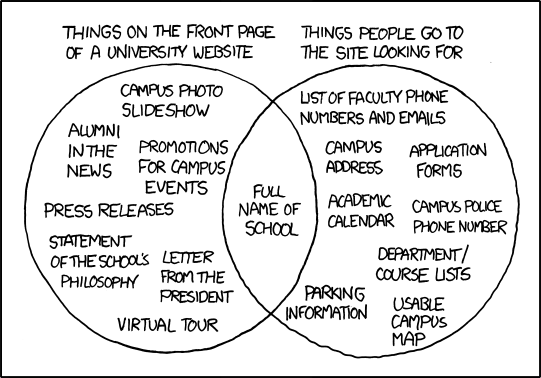
\includegraphics[scale=.65]{comics/733}
\end{center}

\begin{itemize}\itemsep 0pt
    \item Bachelor Mathematik\\
          \url{https://mailman.rrz.uni-hamburg.de/mailman/listinfo/bama}
    \item Bachelor Wirtschaftsmathematik\\
          \url{https://mailman.rrz.uni-hamburg.de/mailman/listinfo/bawima}
    \item Lehramt an Gymnasien und Berufliche Schulen\\
          \url{https://mailman.rrz.uni-hamburg.de/mailman/listinfo/lamagymbs}
    \item Lehramt an der Primar- und Sekundarstufe I, Lehramt an
          Sonderschulen\\
          \url{https://mailman.rrz.uni-hamburg.de/mailman/listinfo/lamapss}
\end{itemize}

Wenn ihr euch mit Professoren oder anderen Mitarbeitern treffen wollt, ist es
häufig sinnvoll, den Kontakt zunächst per E-Mail herzustellen und dann einen
Termin abzusprechen. Wegen kleinerer Angelegenheiten kann man die meisten
Professoren bei deren Anwesenheit häufig auch außerhalb der Sprechstunden
aufsuchen.
\end{multicols}

\subsubsection{Studienfachberatung}

%% Informationen sind online unter
%% http://www.math.uni-hamburg.de/teaching/service/studienfachberatung.html
%% zu finden.

\begin{tabularx}{\textwidth}{|X|X|X|X|}
\hline Bachelor Mathematik&Studienbüro Mathematik&Di, Mi, Do \hfill 10-12
    &Räume E 14, E16\\
    &studienbuero@math.uni-hamburg.de&Di, Do \hfill13-15&\\
\hline Bachelor Wirtschaftsmathematik&Prof. Dr. Hans Daduna&Di \hfill 10-11
    &Raum T17 \\
&hans.daduna@math.uni-hamburg.de&&+49 40 42838-4930\\
&&&\\
&Prof. Dr. Natalie Neumeyer&Di \hfill 14-15&Raum T13\\
&natalie.neumeyer@math.uni-hamburg.de&&+49 40 42838-4907\\
\hline Bachelor Lehramtsstudiengänge&&&\\
Lehramt Gymnasium und Berufliche Schulen&Prof. Dr. Ingo Runkel&&Raum 309\\
    &ingo.runkel@math.uni-hamburg.de&&+49 40 42838-5172\\
&&&\\
Lehramt Primar- und Sekundarstufe I, Lehramt an Sonderschulen
    &Prof. Dr. Andrea Blunck&Di \hfill 14-15&Raum 211\\
    &andrea.blunck@math.uni-hamburg.de&&+49 40 42838-5160\\
&&&\\
\hline Master Mathematik
    &\multicolumn{3}{|l|}{Studienbüro Mathematik, siehe Bachelor Mathematik}\\
\hline
\end{tabularx}

\subsubsection{Spezielle Fragen zu den Prüfungen für das Lehramt}

\begin{tabularx}{\textwidth}{|X|X|X|X|}
\hline Lehrerprüfungsamt&Mümmelmannsberg 75&Mo, Do \hfill 9-12
    &+49 04 42854-7611\\
    &&Di \hfill 14-15&\\
\hline
\end{tabularx}

\subsubsection{BAföG-Vertrauensdozenten}

\begin{tabularx}{\textwidth}{|X|X|X|}
\hline Prof. Dr. Hans Joachim Oberle&Di,Fr \hfill 9-10&Raum 120\\
       oberle@math.uni-hamburg.de&&+49 40 42838-5113\\
\hline Prof. Dr. Thomas Andreae&Di, Fr \hfill 14-15&Raum 238\\
       andreae@math.uni-hamburg.de&&+49 40 42838-5196\\
\hline
\end{tabularx}

\subsubsection{Beauftragter für ausländische Studierende}

\begin{tabularx}{\textwidth}{|X|X|X|}
\hline Prof. Dr. Ingenuin Gasser&Di \hfill 11-12&Raum 105\\
       ingenuin.gasser@math.uni-hamburg.de&&+49 40 42838-5128\\
\hline
\end{tabularx}

\subsubsection{Fachschaftsrat Mathematik}

\begin{tabularx}{\textwidth}{|X|X|X|}
\hline Fachschaftsrat Mathematik&&Raum T30\\
       fsr@math.uni-hamburg.de&&\\
\hline
\end{tabularx}

\subsubsection{Wichtige Adressen und Telefonnummern}

\begin{tabularx}{\textwidth}{|X|X|X|X|}
\hline FSR Wirtschaftswissenschaften&Von-Melle-Park 5&Raum 0070&+49 40 441266\\
       \url{http://wiwifsr.de/}&&&\\
\hline FSR Physik&Jungiusstraße 9&Raum 020&+49 40 352 202\\
       \url{http://fsrix.physnet.uni-hamburg.de/}&&&\\
\hline FSR Informatik&Vogt-Kölln-Str. 30&C-215&+49 40 5404228\\
\url{http://www.informatik.uni-hamburg.de/Fachschaft/wiki/index.php/Fachschaftsrat}&&&\\
\hline FSR Elektrotechnik&Schwarzenbergstraße 95&Raum E 0.098&+49 40 42878-2975\\
       \url{http://fsr-etit.de/}&&&\\
\hline FSR Maschinenbau&Schwarzenbergstraße 95&Raum 0.101&+49 40 42878-4008\\
       \url{http://cgi.tu-harburg.de/~fsrmwww/doku.php?id=start}&&&\\
\hline Studierendenwerk Hamburg&Von-Melle-Park 2&&+49 40 41902-0\\
       \url{http://www.studierendenwerk-hamburg.de}&&&\\
\hline
\end{tabularx}
\clearpage


\section{Lehrveranstaltungen}
\begin{tabularx}{\textwidth}{|l|X|X|X|}
% I. Bachelor (Mathematik, Wirtschaftsmathematik, Mathematik Lehramt an Gymnasien und Lehramt an Beruflichen Schulen)
\hline 65--001 	& Orientierungseinheit f"ur Studienanf"anger/innen (Mathematik und Wirtschaftsmathematik Bachelor, alle Lehr"amter mit Mathematik als Unterrichtsfach)
			& Block\-ver\-an\-stal\-tung vom 04.-13.10.12; 4 SWS, ganzt"agig, Beginn: 04.10.12, 09:30 Uhr Geom H1
			& Dr. Hubert Kiechle, Martin Rybicki \\
\hline 65--002 	& Tutorium f"ur ausl"andische Studierende (insbesondere im Rahmen von ERASMUS)
			& 2 SWS, Zeitpunkt noch unbekannt
			& Prof. Dr. Armin Iske \\
\hline 65--003 	& Vorkurs Mathematik (Blockveranstaltung vom 24.09 - 02.10.12)
			& 2,83 SWS, Mo.-Do. 09:30-11:00, 11:30-13:00, 17:00-18:15, Fr. 09:30-11:00, 11:30-13:00, 16:15-17:30, Mo. 01.10.-Di. 02.10. 09:30-11:00, 11:30-13:00, 16:15-17:30, Hörsaal C Chemie, Beginn 24.09.2012
			& Dr. Anna Posingies \\
\hline 65--004 	& "Ubungen zu Vorkurs Mathematik (Blockveranstaltung vom 24.09.-02.10.12) (7 Gruppen)
			& 1 SWS, Mo.-Do. 15:15-16:45, Fr. 14:15-15:45, Mo. 01.10.-Di. 02.10. 14:15-15:45, Geom 241, 430, 431, 432, 434, 435, 1240
			& N.N. \\
\hhline{|=|=|=|=|} 65--011 & Lineare Algebra und Analytische Geometrie I
			& 4 SWS, Mo. 14:15-15:45, Mi. 08:15-09:45, Geom H1, Beginn: 15.10.12
			& Prof. Dr. Birgit Richter \\
\hline 65--012 	& "Ubungen zu Lineare Algebra und Analytische Geometrie I (10 Gruppen)
			& 2 SWS, Di. 14:15-15:45, Geom 241, 435, Di. 16:15-17:45, Geom 435, 1240, Mi. 10:15-11:45, Geom 434, (431, 435 f"ur LG/LBS), Mi. 12:15-13:45, Geom 431, 434, 435, Beginn: 16.-17.10.12
			& Prof. Dr. Birgit Richter, N.N. \\
\hline 65--014 	& Tutorium zu Lineare Algebra und Analytische Geometrie I (9 Gruppen)
			& 1 SWS, Mo. 12:15-13:00, Geom 434, 435 (\& 431 f"ur LG/LBS), Mo. 13:15-14:00, Geom 435 (\& 431 f"ur LG/LBS), Di. 12:15-13:00, Geom 241, 430, Di. 13:15-14:00, Geom 241, 430, Beginn: 15.-16.10.12
			& N.N. \\
\hline 65--021 	& Analysis I
			& 4 SWS, Mi. 14:15-15:45, Fr. 14:15-15:45 Geom H1, Beginn: 17.10.12
			& Prof. Dr. Timo Reis \\
\hline 65--022 	& "Ubungen zu Analysis I (9 Gruppen)
			& 2 SWS, Do. 08:15-09:45, Geom 241, 1240, Do. 10:15-11:45, Geom 241, 431, 1240, Fr. 08:15-09:45, Geom 241, 431, Fr. 16:15-17:45, Geom 431, 435 (LG/LBS), Beginn: 17.-19.10.12
			& Prof. Dr. Timo Reis, N.N. \\
\hline 65--024 	& Tutorium zu Analysis I (5 Gruppen)
			& 2 SWS, Do. 08:15-09:45, Geom 431, (435 LG/LBS), Do. 12:15-13:45, Geom 431, (435 LG/LBS), Do. 14:15-15:45, Geom 431, Beginn: 18.10.12
			& N.N. \\
\hline
\end{tabularx}
\begin{tabularx}{\textwidth}{|l|X|X|X|}
%Keine Markierung, welche LG/LBS sind.
% II. Bachelor (Mathematik Lehramt der Primarstufe und Sekundarstufe I sowie Lehramt an Sonderschulen)
\hline 65--301 	& Grundlagen der Mathematik
			& 4 SWS, Mo. 14:15-15:45, Mi. 08:15-09:45, Geom H2, Beginn: 15.10.10
			& Dr. Hubert Kiechle \\
\hline 65--302 & "Ubungen zu Grundlagen der Mathematik (5 Gruppen)
			& 2 SWS, Mo. 16:15-17:45, Geom 241, 431, 435, 1240, Di. 14:15-15:45, Geom 1240, Beginn: 15.-16.10.12
			& Dr. Hubert Kiechle, N.N. \\
% Enthalten oben.
%\hline 65-252 & "Ubungen zu Grundlagen der Mathematik f"ur Studierende der Lehr"amter Primarstufe und Sekundarstufe I sowie Sonderschulen (5 Gruppen)
%              & 2st., Mo 16.15-17.45 Geom 431,434,435,1241,Di 14.15-15.45 Geom 1241 Beginn: 19.10.10
%              & Hans-Joachim Samaga\\
% Ist aktuell. (Stand 18.9.2010)
\hline 65--324 & Arbeitsgruppenbetreuung zu Grundlagen der Mathematik, Grundbildung Analysis und Grundbildung Stochastik (5 Gruppen)
			& 4 SWS, Do. 18:00-21:00, Geom 430, 431, 432, 434, 435, Beginn: 18.10.12
			& Dr. Hans-Christian von Bothmer, Dr. Hubert Kiechle, Dr. Susanne Margret Koch \\
%entf"allt.
%\hhline{|=|=|=|=|} 65--902	& Geschichte der Mathematik
%			& 2 St., Fr. 12.15 - 13.45, Geom H1, Beginn: 22.10.10
%			& Prof. Dr. Thomas Sonar \\
%
%\hline 65--922	 & Seminar zur Vorlesung 65--902: Geschichte der Mathematik
%			& 2 St., Fr. 14:15 - 15:45, Geom E11/13, Beginn: 22.10.10
%			& Prof. Dr. Thomas Sonar \\

% III. Master (Mathematik Lehramt der Primarstufe und Sekundarstufe I sowie Lehramt an Sonderschulen)%\hline 65--303 & Frauen in der Geschichte der Mathematik
%			& 2 St., Do. 14:45 - 15:45, Geom H4, Beginn: 21.10.10
%			& Prof. Dr. Andrea Blunck \\
%
%\hline 65--304 & "Ubungen zu Frauen in der Geschichte der Mathematik (2 Gruppen)
%			& 1 St., Do. 12:15 - 13:45, Geom H3, Beginn: 28.10.10
%			& Prof. Dr. Andrea Blunck \\
% IV, V, VI, VII fehlen! (TODO)
% Nebenfach: Physik
\hhline{|=|=|=|=|} 66--100 	& Physik I
			& 4 SWS, Di. 14:00-15:30, Do. 09:00-10:30, Jungius 9, H"ors II, Beginn: 23.10.12
			& Prof. Dr. Ulrich Merkt \\
\hline 66--101 	& Einf"uhrung in die Theoretische Physik I
			& 3 SWS, Di. 15.45-16.45, Do. 10.45-12.00, Jungius 9, H"ors II, Beginn: 23.10.12
			& Prof. Dr. Ludwig Mathey \\
\hline 66--102 	& "Ubungen zur Physik I und Einf"uhrung in die Theoretische Physik I
			& 3 SWS, Do. 13.00-15.15, 15.30-17.45, 18:00-20:15, Jungius 9 Bibliothek AP, SemRm 3, 4, 5, 6, Beginn: 01.11.12
			& Prof. Dr. Ulrich Merkt, Prof. Dr. Ludwig Mathey, Daniela Pfannkuche, Thorsten Uphues, N.N. \\
\hline 66--103	& Tutorium zur Physik I und Einf"uhrung in die Theoretische Physik I
			& 2 SWS, keine Angaben (bei Studienbeginn unter www.physnet.uni-hamburg.de einsehbar), Hinweise in den Lehrveranstaltungen 66-100, 66-101, 66-102, Beginn: 3. Vorlesungswoche
			& Prof. Dr. Ulrich Merkt, Prof. Dr. Ludwig Mathey \\

% Nebenfach: Informatik
\hhline{|=|=|=|=|} 64--000 & Vorlesung Softwareentwicklung I
			& 2 SWS, Mi. 14:15-15:45, H"orsaal Chemie A, Beginn: 17.10.12
			& Dr. Axel Schmolitzky \\
\hline 64--001 & "Ubungen zu Softwareentwicklung I (7 Gruppen)
			& 2 SWS, Mo. 09:00-12:00, Di. 09:00-12:00, 14:00 - 17:00, Mi. 09:00-12:00, Do. 09:00-12:00, 14:00-17:00, Fr. 09:00-12:00, D-010, D-017, D-018, D-114, Beginn: 18.-24.10.12
			& Dr. Axel Schmolitzky, Christian Sp"ah, Till Aust, Philip Joschko, Arne Koors, Sven Magg, Fredrik Winkler, Claudia Wyrwoll, Christin Zahner \\
\hline 64-070 & Vorlesung Algorithmen und Datenstrukturen
			& 3 SWS, Mi. 10:15-11:45,Phil C, Fr. 14:15-15:45, Phil B, Beginn: 17.10.12
			& Prof. Dr. Matthias Rarey \\
\hline 64-071 & "Ubungen zu Algorithmen und Datenstrukturen (10 Gruppen)
			& 1 SWS, Mi. 12:15-13:45, F-009, Mi. 14:15-15:45, ZBH Rm 16, F-635, F-534, Mi. 16:15-17:45, D-129, F-534, Do. 10:15-11:45, F-534, F-334, Fr. 10:15-11:45, 12:15-13:45, ZBH Rm 16, Beginn: 19.-26.10.12
			& Mathias Michael von Behren, Matthias Hilbis, Matthias Kerzel, Florian Lauck, Thomas Wagner, N.N. \\

% Gibt es nicht mehr.
%\hline 64-080 & Vorlesung Grundlagen von Datenbanken (GDB) (Modul IP5)
%              & 3st. Mi 10:15-11:45, MLK6 HsB Chem Di 14:15 15:45, VMP8 Erzwiss H, Beginn: 21.10.09
%              & Norbert Ritter \\
%
%\hline 64-081 & "Ubung zu Grundlagen von Datenbanken (Modul IP5)
%              & 1st. Mo 10:15-11:45 Mo 12:15-13:45 Mo 14:15-15:45 Di 8:15-9:45 Di 10:15-11:45, Beginn 19.10.09
%              & Norbert Ritter, Marc Holze, Fabian Panse, Michael von Riegen \\
			&&&\\
\hline
\end{tabularx}

F"ur Informatik waren dies nur einige der zu empfehlenden VeranstaltungenWeitere Informatik-Vorlesungen siehe\url{www.informatik.uni-hamburg.de/Info/Studium}.

\begin{tabularx}{\textwidth}{|l|X|X|X|}
% Nebenfach: VWL / BWL?
\hline 21-10.010 & Grundlagen des Rechnungswesens - Z1
			& 3 SWS, Di. 09:00 - 12:00, Audimax 1, Beginn: 16.10.12
			& Dr. Andreas Mammen \\
\hline 21-10.010 & "Ubungen zu Grundlagen des Rechnungswesens - Z1  (10 Gruppen)
			& 1 SWS, Mo. 13:00-14:00, WiWi B1, WiWi 3136/3142 (30 Plätze für Holzwirte), Di. 08:00-09:00, WiWi 2101/2105 (nur für Wi-Ing), WiWi 2098/2194, Di. 15:00-16:00, WiWi 2163/2168 (nur für Wi-Ing), WiWi 2091/2201, Mi. 16:00-17:00, WiWi 2067/2071, 2091/2201, Mi. 17:00-18:00, WiWi 2067/2071, 2091/2201, Beginn: 22.-24.10.12
			& Dr. Andreas Mammen \\
\hline 21-10.011 & Grundlagen des Rechnungswesens - Z2
			& 3 SWS, Mo 10:00-13:00, Audimax 1, Beginn: 15.10.12
			& Dr. Ralf Wi"smann \\
\hline 21-10.011 & "Ubungen zu Grundlagen des Rechnungswesens - Z2 (10 Gruppen)
			& 1 SWS, Mo. 09:00-10:00, WiWi 0029, WiWi 2163/2168, Di. 17:00-18:00, WiWi 0029, 2163/2168, Di. 18:00-19:00, WiWi 0029, 2163/2168, Fr. 08:00-09:00, WiWi 0079, WiWi 2067/2071 (nur für LL.bB. Arbeits- + Sozialmanagement und LL.B. Finanzen + Versicherung), Fr. 16:00
			-17:00, WiWi 2095/2197, 2101/2105, Beginn: 22.-23./26.10.12
			& Dr, Ralf Wi"smann \\
\hline 21-10.020 & Grundlagen der Wirtschaftsinformatik - Z1
			& 2 SWS, Mo. 10:00-12:00, Erzwiss H, Beginn: 15.10.12
			& Dr. Gabriele Schneidereit, Dr. Silvia Schwarze \\
\hline 21-10.020 & "Ubungen zu Grundlagen der Wirtschaftsinformatik - Z1 (6 Gruppen)
			& 2 SWS, Mo. 08:00-10:00, WiWi 2067/2071, 2091/2201, Do. 10:00-12:00 WiWi 2091/2201, 2095/2197, Fr. 14:00-16:00 WiWi 2091/2201, 2101/2105, Beginn: 22./25.-26.10.12
			& Dr. Gabriele Schneidereit, Dr. Silvia Schwarze \\
\hline 21-10.021 & Grundlagen der Wirtschaftsinformatik - Z2
			& 2 SWS, Di. 10:00-12:00, Erzwiss H, Beginn: 16.10.12
			& Dr. Kai Br"ussau, Dr. Gabriele Schneidereit \\
\hline 21-10.021 & "Ubungen zu Grundlagen der Wirtschaftsinformatik - Z2 (8 Gruppen)
			& 2 SWS., Di. 08:00-10:00, WiWi 0079, 2091/2201, Mi. 10:00-12:00, WiWi 2054/2055, 2091/2201, Mi. 16:00-18:00, WiWi 2054/2055, 2163/2168, Do. 12:00-14:00, WiWi 2091/2201, 2095/2197, Beginn: 23.-25.10.12
			& Dr. Kai Br"ussau, Dr. Gabriele Schneidereit, Dr. Robert Stahlbock, Stefan Lessmann \\

% Nebenfach: TUHH? (TODO)
%\hhline{|=|=|=|=|} TUHH & Grundlagen der Elektrotechnik I
%                        & Donnerstag, 11:30-13 in H - SBS95 Raum Audimax1
%                        & G"unter Ackermann \\
%
%&&&\\
%
%\hline TUHH & Elektrotechnik I / Grundlagen der Elektrotechnik I
%            & Montag, 8:00-9:30 in I - DE22 Raum Audimax2, Donnerstag, 11:30-12:45 in I - DE22 Raum Audimax2
%            & Jan-Luiken ter Haseborg \\%%\hline TUHH & Technische Mechanik I
%            & Mittwoch, 8:00-9:30 in I - DE22 Raum Audimax2
%            & Uwe Weltin \\
\hline
\end{tabularx}
\begin{tabularx}{\textwidth}{|l|X|X|X|}
\hline 21-10.095 & Makro"okonomik - Z1
			& 3 SWS, Fr. 09:00-12:00, Audimax 1, Beginn: 19.10.12
			& Dr. Sven Schreiber \\
\hline 21-10.095 & "Ubungen zu Makro"okonomik (8 Gruppen)
			& 1 SWS, Mo. 13:00-14:00, WiWi 2067/2071, 2091/2201, Mi. 09:00-10:00, WiWi 2101/2105, 2067/2071, Mi. 11:00-12:00, WiWi 2163/2168, 2095/2197, Fr. 13:00-14:00, WiWi 2091/2201, 2095/2197, Beginn: 22./24./26.10.12
			& Dr. Sven Schreiber \\
\hline 21-10.096 & Makro"okonomik - Z2
			& 3 SWS, Do. 8:00-11:00, Audimax 1, Beginn: 18.10.12
			& Prof. Dr. Lena Dräger \\
\hline 21-10.096 & "Ubungen zu Makro"okonomik - Z2 (8 Gruppen)
			& 1 SWS, Mo. 12:00-13:00, WiWi 2067/2071, 2091/2201, Mi. 08:00-09:00, WiWi 2101/2105, 2067/2071, Mi. 10:00-11:00, WiWi 2163/2168, 2095/2197, Fr. 12:00-13:00, WiWi 2091/2201, 2095/2197 (für Wirtschaft und Kultur Chinas u. LL. B. Arbeits- und Sozialmanagement), Beginn: 22./24./26.10.12
			& Prof. Dr. Lena Dräger \\
\hline 21-10.110 & Investition - Z1
			& 2 SWS, Do 16:00-18:00, ESA A, Beginn: 18.10.12
			& Prof. Dr. Martin Nell \\
\hline 21-10.110 & "Ubungen zu Investition - Z1 (8 Gruppen)
			& 2 SWS, Mo. 15:00-17:00, WiWi 2098/2194, 3136/3142, Di. 12:00-14:00, WiWi 2095/2197, 3136/3142 (beide für Wi-Ing), Mi. 12:00-14:00, WiWi 2098/2194, 3136/3142, Do. 08:00-10:00, WiWi 2098/2194, 2095/2197 (40 Plätze für LL.B. Finanzen und Versicherung), Beginn: 22.-25.10.12
			& Prof. Dr. Martin Nell \\
\hline 21-10.111 & Investition - Z2
			& 2 SWS, Do. 14:00-16:00, ESA A, Beginn: 18.10.12
			& Prof. Dr. Martin Nell \\
\hline 21-10.111 & "Ubungen zu Investition - Z2 (8 Gruppen)
			& 2 SWS, Mo. 08:00-10:00, 10:00-12:00, WiWi 2098/2194, 3136/3142, Mi. 15:00-17:00, WiWi 2098/2194, 2101/2105, Do. 12:00-14:00, WiWi 2067/2071, 2098/2194, Beginn: 22./24.-25.10.12
			& Prof. Dr. Martin Nell \\
\hline
\end{tabularx}


\section{Abkürzungsverzeichnis}
\begin{multicols}{3}
\scriptsize

\begin{tabular}{|p{10mm} p{68mm}|}
\hline
AG     	& Arbeitsgemeinschaft/-gruppe \\
Aküvz  	& Abkürzungsverzeichnis \\
AP     	& Allende-Platz (am Grindelhof) \\
AS     	& Akademischer Senat \\
AStA   	& Allgemeiner Studierendenausschuss \\
BAföG 	& Bundesausbildungsförderungsgesetz \\
BaMa		& Bachelor-MathematikerIn \\
BdMN    & Bibliothek der Mathematik und\\
       	& Naturwissenschaften \\
Bem.   	& Bemerkung \\
Bib			& Bibliohek \\
B.Sc.		& Bachelor of Science \\
BMGN		& Bibliothek für Mathematik und Geschichte der Naturwissenschaften \\
BWL    	& Betriebswirtschaftslehre \\
bzw.   	& beziehungsweise \\
c.t.   	& cum tempore (mit akadem. Viertel) \\
cosh   	& hyperbolischer Kosinus \\
Def.   	& Definiton \\
d.h.   	& das heißt \\
Doz.   	& DozentIn \\
ESA    	& Edmund-Siemers-Allee (Universitäts\-haupt\-gebäude am Dammtor) \\
etc.   	& et cetera (und weitere) \\
FA			& Fachausschuss \\
Fak			& Fakultät \\
FB     	& Fachbereich \\
FBR    	& Fachbereichsrat \\
FSR    	& Fachschaftsrat (oder -raum = T30) \\
FSRK   	& Fachschaftsrätekonferenz \\
FSZ    	& Fachsprachenzentrum \\
GEZ    	& Gebühreneinzugszentrale \\
GruMi  	& Studierende(r) des Lehramts der Grund- und Mittelstufe \\
HOE    	& Hauptstudiums-OE \\
H1-H6  	& Hörsäle des Geomatikums \\
HSG    	& Hochschulgruppe (meist ein politischer Ableger einer \glqq real existierenden\grqq\ Partei) \\
HVV    	& Hamburger Verkehrsverbund \\
HWP     & Hochschule für Wirtschaft und Politik \\
IGN    	& Institut für Geschichte der Naturwissenschaften, Mathematik und Technik \\
IZHD   	& Interdisziplinäres Zentrum für Hochschuldidaktik \\
KoMa   	& Konferenz der deutschsprachigen Mathematikfachschaften \\
KVV    	& Kommentiertes Vorlesungsverzeichnis \\
L\&L    & Lehr- und Lernformen \\
Lem.   	& \raisebox{0pt}[2.65mm]{Lemma, mathematische Hilfsaussage} \\
\hline
\end{tabular}

\begin{tabular}{|p{10mm} p{68mm}|}
\hline
\LaTeX 	& [\textipa{la:tEX}] Textsatzprogramm \\
lim     & Limes \\
ln      & natürlicher Logarithmus \\
M\&G    & Mathematik und Gesellschaft \\
max.    & maximal \\
min.    & mindestens; minimal; Minuten \\
MLKP   	& Martin-Luther-King-Platz (zw. Chemie und Zoologie) \\
NuMa    & (Nur-)MathematikerIn (BaMa) \\
N.N.		& nomen nominandum (\textit{lat.} zu nennender Name) \\
o.ä.  	& oder ähnlich \\
OE     	& Orientierungseinheit \\
Philturm & Philosophenturm \\
PI     	& (Gebäude des) Fachbereichs Erzieh\-ungs\-wissenschaften \\
POE    	& Problemorientierte Einführung \\
q.e.d. 	& quod erat demonstrandum (was zu beweisen war) \\
SIV    	& Studentische Interessensvertretung \\
SoSe   	& Sommersemester (auch SS) \\
SP     	& Schwerpunkt \\
SP AD  	& SP Analysis \& Differentialgeometrie \\
SP AZ  	& SP Algebra \& Zahlentheorie \\
SP DD  	& SP Differentialgleichungen \& Dynamische Systeme \\
SP GD  	& SP Geometrie \& Diskrete Mathematik \\
SP GN  	& SP Geschichte der Naturwissenschaften, Mathematik und Technik \\
SP OA  	& SP Optimierung \& Approximation \\
SP ST  	& SP Mathematische Statistik \& Stochastische Prozesse \\
SPR   	& Schwerpunktsrat\\
s.t.		& sin tempore (ohne akadem. Viertel) \\
StaBi  	& Staatsbibliothek \\
StuPa   & Studierendenparlament \\
SWS    	& Semesterwochenstunde(n) \\
tanh   	& hyperbolischer Tangens \\
TeMa   	& TechnomatematikerIn \\
\TeX   	& [\textipa{tEX}] Textsatzprogramm \\
TVP    	& Technisches und Verwaltungspersonal \\
u.     	& und \\
u.U.   	& unter Umständen \\
Übi   	& ÜbungsgruppenleiterIn \\
ÜG			& Übungsgruppe \\
UKE    	& Universitätklinikum Eppendorf \\
usw.   	& und so weiter \\
VMP    	& Von-Melle-Park (= Campusgelände) \\
Vorl.		& Vorlesung \\
VV     	& Vollversammlung; Vorlesungsverzeichnis \\
VWL    	& Volkswirtschaftslehre \\
\hline
\end{tabular}

\begin{tabular}{|p{10mm} p{68mm}|}
\hline
WiMa   	& WirtschaftsmathematikerIn \\
WiSe   	& Wintersemester (auch WS) \\
WiWi   	& Wirtschaftswissenschaften (auch WiWi-Bunker) \\
z.B.   	& zum Beispiel \\
ZBMI   	& Zentralbibliothek der Mathematischen Institute\\
ZMP			& Zentrum für Mathematische Physik \\
ZMS    	& Zentrum für Modellierung \& Simulation \\
zw.    	& zwischen \\
\hline
\end{tabular}

% TODO: Fugly.

\vspace{1.45mm}

\begin{tabular}{|llp{21.75mm}|llp{21.75mm}|}

\hline
\multicolumn{6}{|c|}{Griechische Buchstaben} \\
\hline

\textit{A}       & $\alpha$                   & Alpha
    & \textit{N} & $\nu$                      & Nü       \\
\textit{B}       & $\beta$                    & Beta
    & $\Xi$      & $\xi$                      & Xi       \\
$\Gamma$         & $\gamma$                   & Gamma
    & \textit{O} & \textit{o}                 & Omikron  \\
$\Delta$         & $\delta$                   & Delta
    & $\Pi$      & $\pi$,      $\varpi$       & Pi       \\
\textit{E}       & $\epsilon$, $\varepsilon$  & Epsilon
    &\textit{P}  & $\rho$,     $\varrho$      & Rho      \\
\textit{Z}       & $\zeta$                    & Zeta
    & $\Sigma$   & $\sigma$,   $\varsigma$    & Sigma    \\
\textit{H}       & $\eta$                     & Eta
    & \textit{T} & $\tau$                     & Tau      \\
\textit{T}       & $\theta$,   $\vartheta$    & Theta
    & \textit{Y} & $\upsilon$                 & Ypsilon  \\
\textit{I}       & $\iota$                    & Iota
    & $\Phi$     & $\phi$,     $\varphi$      & Phi      \\
\textit{K}       & $\kappa$,   $\varkappa$    &Kappa
    & \textit{X} & $\chi$                     & Chi      \\
$\Lambda$        & $\lambda$                  & Lambda
    & $\Psi$     & $\psi$                     & Psi      \\
\textit{M}       & $\mu$                      & Mü
    & $\Omega$   & $\omega$                   & Omega    \\
\hline
\multicolumn{6}{|c|}{Hebräische Buchstaben} \\
\hline

$\aleph$            && Aleph   & {\fonti\char'151} && Beth    \\
{\fonti\char'152}   && Gimel   & {\fonti\char'153} && Daleth  \\

\hline
\multicolumn{6}{|c|}{Deutsche Buchstaben (Sütterlin)} \\
\hline

{\suetterlin A} & {\suetterlin a} & A
    & {\suetterlin N} & {\suetterlin n} & N \\
{\suetterlin B} & {\suetterlin b} & B
    & {\suetterlin O} & {\suetterlin o} & O \\
{\suetterlin C} & {\suetterlin c} & C
    & {\suetterlin P} & {\suetterlin p} & P \\
{\suetterlin D} & {\suetterlin d} & D
    & {\suetterlin Q} & {\suetterlin q} & Q \\
{\suetterlin E} & {\suetterlin e} & E
    & {\suetterlin R} & {\suetterlin r} & R \\
{\suetterlin F} & {\suetterlin f} & F
    & {\suetterlin S} & {\suetterlin s, \char255} & S, ß \\
{\suetterlin G} & {\suetterlin g} & G
    & {\suetterlin T} & {\suetterlin t} & T \\
{\suetterlin H} & {\suetterlin h} & H
    & {\suetterlin U} & {\suetterlin u} & U \\
{\suetterlin I} & {\suetterlin i} & I
    & {\suetterlin V} & {\suetterlin v} & V \\
{\suetterlin J} & {\suetterlin j} & J
    & {\suetterlin W} & {\suetterlin w} & W \\
{\suetterlin K} & {\suetterlin k} & K
    & {\suetterlin X} & {\suetterlin x} & X \\
{\suetterlin L} & {\suetterlin l} & L
    & {\suetterlin Y} & {\suetterlin y} & Y \\
{\suetterlin M} & {\suetterlin m} & M
    & {\suetterlin Z} & {\suetterlin z} & Z \\
\hline \end{tabular}

% TODO: Fugly.

\vspace{1.45mm}

\begin{tabular}{|l|p{75.85mm}|}
\hline
$\mathbb C$ & Komplexe Zahlen\\
$\mathbb H$ & Hamiltonsche Quaternionen\\
$\mathbb K$ & allg. Körper, häufig $\mathbb R$ od. $\mathbb C$\\
$\mathbb N$ & Natürliche Zahlen\\
$\mathbb O$ & Oktonionen\\
$\mathbb Q$ & Rationale Zahlen\\
$\mathbb R$ & Reelle Zahlen\\
$\mathbb Z$ & Ganze Zahlen\\
\hline
\end{tabular}

\normalsize

\end{multicols}

\section{Allgemeine Warnhinweise}
\begin{multicols}{2}[\subsection{Allgemeine Warnhinweise zur Benutzung dieses
Laptops}]

Die rasante Entwicklung der Wissenschaft in den letzten Jahrzehnten hat uns
gewaltige technische Fortschritte gebracht. Die neuen Produkte geben uns nicht
nur mehr Annehmlichkeiten und Komfort, sondern können auch bisher nicht
gekannte Risiken mit sich bringen.

Aus diesem Grunde hat die EU-Kommission eine Gruppe von hochrangigen
Wissenschaftlern beauftragt, mithilfe der neuesten Erkenntnisse die Gefahren
und Risiken zu identifizieren, die dank der Wissenschaft nunmehr erkennbar
geworden sind.

Mithilfe des Abschlussberichtes wurden dann in einem eigens dazu eingerichteten
Ausschuss aus Gewerkschaften, Verbraucherschützern und Verwaltungsbeamten
Warnhinweise entwickelt, die ab dem 1.8.2003 auf jedem in der EU in Verkehr
gebrachten Produkt angebracht werden müssen.

Für das Benutzen dieser Informationsbroschüre des Fachbereichs Mathematik ist
somit folgendes zu beachten:

\important Dieses Produkt krümmt Raum und Zeit in seiner Umgebung!

\important Dieses Produkt zieht die gesamte Materie des Universums mit einer
Kraft an, die dem Produkt der Massen proportional ist und mit dem Quadrat der
Entfernung abnimmt!

\important Die Masse dieses Produkts enthält das Energieäquivalent von 30
Millionen Tonnen TNT pro Gramm!

\important In diesem Produkt bewegen sich kleinste elektrisch geladene Teilchen
mit einer Geschwindigkeit von mehr als 800 Millionen km/h!

\important Es besteht die Möglichkeit, dass dieses Produkt durch einen Prozess,
der als \emph{Tunneln} bekannt ist, von seinem Platz verschwindet und an einer
anderen Stelle des Universums wieder auftaucht. Der Herausgeber ist weder für
daraus entstehende Schäden noch für den möglichen Verlust des Gerätes haftbar!

\important Einer Version der großen vereinheitlichten Theorie zufolge können
die Elementarteilchen, aus denen dieses Produkt besteht, in den nächsten 4,5
Milliarden Jahren zu Strahlen zerfallen!

\important Dieses Produkt besteht zu 100\% aus Materie. Im Falle des Kontaktes
mit Antimaterie kommt es zu gefährlichen Explosionen!

\important Die fundamentalen Elementarteilchen, aus denen dieses Produkt
besteht, werden durch eine Kraft zusammengehalten, deren Natur nicht bekannt
ist. Ihr zukünftige Funktion kann daher nicht garantiert werden!

\important Unabhängig von anderen Deklarationen der Inhaltsstoffe bzw. der
Zusammensetzung weisen wir darauf hin, dass dieses Produkt zu 99,99999999\% aus
leerem Raum besteht.

\important Aufgrund quantenmechanischer Effekte kann es sein, dass dieses
Produkt entweder aufhört zu existieren oder in einen unbestimmten Zustand
übergeht, wenn es nicht beobachtet wird. Der Gebrauchswert ist davon jedoch
nicht betroffen.

\important Das gesamte Universum, einschließlich dieses Produktes, kann eines
Tages zu einem unendlich kleinen Punkt kollabieren. Sollte daraus wiederum ein
neues Universum entstehen, kann die Existenz dieses Produktes darin nicht
garantiert werden.

\important Die Gesundheitsminister der EU warnen: Vorsicht beim Heben und
Tragen dieses Produktes! Seine Masse und somit sein Gewicht sind von der
Geschwindigkeit relativ zum Anwender abhängig!

\important Die Innenminister der EU warnen: Jeder Gebrauch dieses Produktes
erhöht die Unordnung im Universum! Dieser Prozess führt mit Sicherheit zum
Wärmetod des Universums!
\end{multicols}


\begin{borderless}
\begin{picture}(0,0)(-7,-8)
\drawline(-3.9,1.6)(9,1.6)(9,5.8)(-3.9,5.8)(-3.9,1.6)
\put(5,-20){\Huge$\bullet$} \put(245,-20){\Huge$\bullet$}
\put(245,-160){\Huge$\bullet$} \put(5,-160){\Huge$\bullet$}
\drawline(280,-100)(170,-100)(170,-160)(164,-160)(164,-167)(170,-167)
\drawline(170,-167)(170,-193)(280,-193)
\drawline(280,-100.4)(170.4,-100.4)(170.4,-160.4)(164.4,-160.4)(164.4,-166.6)(170.4,-166.6)
\drawline(170.4,-166.6)(170.4,-192.6)(280,-192.6)
\put(165.5,-164.7){\Large$\otimes$}
\put(266,-147){\Large$\Biggr)$} \put(267,-147){\Large$\Biggr)$}
\put(268,-147){\Large$\Biggr)$}
\drawline(-9,-200)(-9,-120)(-25,-120)
\drawline(-9.4,-200)(-9.4,-120.4)(-25,-120.4)
\drawline(12,-30)(90,-30)(90,-108)(12,-108)(12,-30)
\drawline(12.4,-30.4)(89.6,-30.4)(89.6,-107.6)(12.4,-107.6)(12.4,-30.4)
\put(50,-45){\Large$\otimes$}
\drawline(22.4,-107.6)(22.4,-103.6)(32.4,-103.6)(32.4,-107.6)
\drawline(79.6,-107.6)(79.6,-103.6)(69.6,-103.6)(69.6,-107.6)
\put(49.7,-30.5){\Large$\frown$} 
\put(170,-52){\Huge --- --- --- --- --- --- --- ---} 
\put(170,-54){\Huge --- --- --- --- --- --- --- ---} 
\put(170,-56){\Huge --- --- --- --- --- --- --- ---}
\put(170,-58){\Huge --- --- --- --- --- --- --- ---}
\put(170,-60){\Huge --- --- --- --- --- --- --- ---}
\put(170,-62){\Huge --- --- --- --- --- --- --- ---}
\put(170,-64){\Huge --- --- --- --- --- --- --- ---}
\put(170,-66){\Huge --- --- --- --- --- --- --- ---}
\put(170,-68){\Huge --- --- --- --- --- --- --- ---}
\put(170,-70){\Huge --- --- --- --- --- --- --- ---}
\put(170,-72){\Huge --- --- --- --- --- --- --- ---}
\put(170,-74){\Huge --- --- --- --- --- --- --- ---}
\put(170,-76){\Huge --- --- --- --- --- --- --- ---}
\put(170,-78){\Huge --- --- --- --- --- --- --- ---}
\put(170,-80){\Huge --- --- --- --- --- --- --- ---}
\drawline(120,-7)(155,-7)(155,-37)(115,-37)(115,-12)(120,-7) 
\tiny
\put(120,-9){MODEL NO:00001b} 
\put(118,-11){TYPE NO: WS10/11}
\put(116,-13){MADE IN HAMBURG 09'07} 
\put(116,-15){MODEM : \makebox[0mm][l]{\hspace*{0.1ex}\raisebox{0.3ex}{/}}$\exists$}
\put(116,-17){FCCRegNo:$H_2O$-$K^oP_f$}
\put(116,-19){Processor:Pentium 0.8.15 $\aleph$Hz}
\put(116,-21){Power Rating: $12+3i$ V}
\put(124.6,-24){\setlength{\fboxsep}{0.2mm}\fbox{\makebox[0mm][l]{\hspace*{0.7ex}\raisebox{0.4ex}{/}}{\fontd\char'100} NOT WASHABLE}}
\put(141,-28){\setlength{\fboxsep}{0.2mm}\fbox{\fontd\char'031\hspace*{0.9ex}+ \fontd\char'032 }} 
\put(116,-35){\fonth{3,14159265358979}}
\put(150.7,-10.7){\fontg{e}} 
\put(150.7,-15.2){\fontg{i}}
\put(150.7,-19.7){\fontg{p}} 
\put(150.7,-24.2){\fontg{=}}
\put(150.7,-28.7){\fontg{1}} 
\put(116,-26.3){Made with \LaTeXe}
\put(116,-29){{\fontd\char'007}0400453168} 
\normalsize
\put(118,-24.4){\fontb\char196}
\end{picture}

\end{borderless}

\end{document}
